    % ----------------------------------------------------------------------------------------------------- %
% Arquivo LaTeX de exemplo de TCC a ser apresentados à Ciência da Computação da UFT - Palmas
% 
% Verssão 2: 20 Fev 2016
%
% Criado por: Tiago Almeida
% Revisado por: 
%  
% ----------------------------------------------------------------------------------------------------- %

\documentclass[tcc2]{uftex}	
\usepackage{float}
\usepackage{pdfpages}
\usepackage[acronym]{glossaries}
\makeglossaries

\usepackage[abnt-emphasize=bf]{abntex2cite}
\citebrackets[]

\renewcommand*{\backrefalt}[4]{}%

\begin{document}
  \title{Implantação da ferramenta para manutenção de serviços ``UFT Serviços'' baseado nas diretrizes do ITIL v3}
  \foreigntitle{Thesis Title}
  \author{Vinícius}{Aires Barros}
  \advisor{Prof.}{Ary}{Henrique Morais de Oliveira}{D.Sc.}

  \examiner{Prof.}{Ary Henrique Morais de Oliveira}{D.Sc.}
  \examiner{Prof.}{Rafael Lima de Carvalho}{D.Sc.}
  \examiner{Prof.}{Thiago Magalhães de Brito Rodrigues}{M.Sc.}
  \department{CC}
  \date{07}{2016}

  \keyword{ITIL v3}
  \keyword{gerenciamento de serviços de TI}
  \keyword{UFT Serviços}
  \keyword{Univsersidade Federal do Tocantins}

  \foreignkeyword{ITIL v3}
  \foreignkeyword{IT service management}
  \foreignkeyword{UFT Serviços}
  \foreignkeyword{Federal University of Tocantins}

  \maketitle
  
  \frontmatter
  
  \includepdf[pages=-]{ficha.pdf}
  
  \includepdf[pages=-]{ata_tccfinal.pdf}
  
  \dedication{Dedico este trabalho em memória ao meu avô Camilo Ayres de Santana e meu tio Adelson Aires Santana.}

  \begin{acknowledgement}

  Primeiramente agradeço a Deus por me permitir vencer mais essa etapa na minha vida, saiba que sem sua imensa misericórdia e seus ensinamentos através da sua palavra eu não conseguiria alcançar os meus objetivos. Agradeço os meus familiares, em especial a minha mãe Sebastiana Aires Santana, pelo apoio dado desde o início da minha jornada nos estudos. Agradeço também aos meus amigos, acima de tudo irmãos que fiz durante minha graduação, em especial ao colega Thaylon Guedes Santos por sua parceria em diversos momentos da graduação, saiba que grande parte do conhecimento adquirido durante a faculdade foi construído através do compartilhamento de informações com você. Agradeço às minhas amigas Adrianne Alves e Valéria Martins por tirarem um pouco do seu tempo para me ajudarem com a revisão da escrita deste trabalho, fornecendo diversas dicas que contribuíram para a finalização e entrega desta monografia. Faço um agradecimento em especial a todos os professores que participaram da minha vida como acadêmico, saibam que sem os seus ensinamentos e orientações eu não conseguiria chegar aonde eu estou. Faço um agradecimento em especial ao professor Tiago Almeida que é um dos professores mais pró-ativos que conheci na graduação, agradeço por sua contribuição através da criação de um modelo padronizado de monografia e por ser um dos poucos professores que se coloca no lugar dos alunos, sendo sempre muito prestativo e atencioso. Agradeço ao meu orientador professor Dr. Ary Henrique Morais de Oliveira por sua orientação e ensinamentos durante a construção desta monografia, saiba que sem sua presença e seus conselhos eu não conseguiria atingir os objetivos deste trabalho. Por fim, dedico esta monografia em memória do meu avô Camilo Ayres de Santana, pessoa que tive como verdadeiro pai durante toda minha infância e início da adolescência, saiba o senhor que sem seus exemplos de luta e perseverança junto a minha a mãe eu não conquistaria mais essa vitória.

  \end{acknowledgement}

  \begin{abstract}
  
  \noindent Este trabalho apresenta os conceitos utilizados para implantação do sistema ``UFT Serviços'' que tem como propósito servir como ferramenta para o gerenciamento de ordem de serviços para a Prefeitura e Direção do Campus de Palmas da Universidade Federal do Tocantins. O ``UFT Serviços'' possui as diretrizes de gerenciamento de serviços de TI da ITIL v3 como ferramenta de apoio às etapas de implantação dos serviços oferecidos pelo \textit{software}. Sua principal motivação é possibilitar uma melhoria na comunicação sobre os problemas de infraestrutura do campus universitário entre a comunidade acadêmica (docente, discente e técnico administrativo) e os setores responsáveis por encaminhamentos das solicitações de reparo. A utilização do ITIL v3, como base para gestão dos serviços oferecidos pelo sistema visa sobretudo proporcionar um melhor controle sobre os problemas relacionados ao desenho e transição dos serviços oferecidos pelo sistema. \\

  \end{abstract}

  \begin{foreignabstract}

  \noindent This work presents the concepts used to implement the ``UFT Serviços'' system. This system is intended to serve as a tool to manage service orders for both the prefecture and campus administration of Palmas in the Federal University of Tocantins. The ``UFT Serviços''  has ITIL v3 guidelines for managing IT services as a support tool to the implementation stages of the services offered by the software. Its main motivation is to enable a communication improvement about the university campus infrastructure problems between academic community (faculty, students and administrative personnel) and the departments responsible for forwarding the repair request. The use of ITIL v3 as a basis for management of the services offered by the system aims above all to provide a better handling of the problems related to the design and transition of the services offered by the system.\\
  
  \end{foreignabstract}

% ----------------------------------------------------------------------------------------------------- %
% Lista de Abreviaturas
% ----------------------------------------------------------------------------------------------------- %

\newacronym{itil}{ITIL}{Information Technology Infrastructure Library}

\newacronym{fgveasp}{FGV-EAESP}{Fundação Getúlio Vargas - Escola de Administração de Empresas de São Paulo}

\newacronym{itsm}{ITSM}{Gerenciamento de Serviços de TI}

\newacronym{ti}{TI}{Tecnologia da Informação}

\newacronym{cobit}{COBIT}{Control Objectives for Information and related Technology}

\newacronym{uft}{UFT}{Universidade Federal do Tocantins}

\newacronym{mandi}{Mandi}{Monitoramento e Análise de Incidentes}

\newacronym{hp}{HP}{Hewlett-Packard}

\newacronym{ibm}{IBM}{International Business Machines Corporation}

\newacronym{idc}{IDC}{International Data Corporation}

\newacronym{ios}{IOS}{Iphone OS}

\newacronym{html}{HTML}{HyperText Markup Language}

\newacronym{css}{CSS}{Cascading Style Sheets}

\newacronym{cobit}{COBIT}{Controle de Objetivos da Informação e Tecnologia Relacionadas}

\newacronym{cmmi}{CMMI}{Capability Maturity Model Integration}

\newacronym{iso}{ISO}{International Organization for Standardization}

\newacronym{rh}{RH}{Recursos Humanos}

\newacronym{jsf}{JSF}{Java Server Faces}

\newacronym{ogc}{OGC}{Office of Goverment Commerce}

\newacronym{itsm}{ITSM}{IT Service Management}

\newacronym{hsmo}{HSMO}{Her Majesty’s Stationery Office}

\newacronym{ccta}{CCTA}{Agência Central de Comunicação e Telecomunicação}

\newacronym{sla}{SLA}{Service Level Agreement}

\newacronym{slm_itil}{SLM}{Service Level Management}

\newacronym{ieee}{IEEE}{Institute of Electrical and Electronics Engineers}

\newacronym{srs}{SRS}{Software Requirements Specification Template}

\newacronym{ism}{ISM}{Information Security Management}

\newacronym{gps}{GPS}{Global Positioning System}

\newacronym{mof}{MOF}{Microsoft Framework}

\newacronym{malssi}{MalSSI}{Managing IT Services and Service Implementation}

\newacronym{uml}{UML}{Unified Modeling Language}

\newacronym{sus}{SUS}{System Usability Scale}

\newacronym{sdk}{SDK}{Software development Kit}

\newacronym{ide}{IDE}{Integrated Development Environment}

\newacronym{http}{HTTP}{Hypertext Transfer Protocol}

\newacronym{qrcode}{QR Code}{Quick Response Code}

\newacronym{jdbc}{JDBC}{Java Database Connectivity}

\newacronym{ejb}{EJB}{Enterprise Java Beans}

\newacronym{rest}{REST}{Representational State Transfer}

\newacronym{javaee}{Java EE}{Java Plataform Enterprise Edition}

\newacronym{jpa}{JPA}{Java Persistence API}

\newacronym{poo}{POO}{Programação Orientada a Objetos}

\newacronym{pojo}{POJO}{Plain Old Java Object}

%\printglossaries
\printglossary[type=\acronymtype,title={Lista de Abreviaturas}]


% ----------------------------------------------------------------------------------------------------- %
% Lista de Figuras
% ----------------------------------------------------------------------------------------------------- %

\listoffigures

% ----------------------------------------------------------------------------------------------------- %
% Lista de Tabelas
% ----------------------------------------------------------------------------------------------------- %

\listoftables

% ----------------------------------------------------------------------------------------------------- %
% Sumário
% ----------------------------------------------------------------------------------------------------- %

\tableofcontents 

\mainmatter
\onehalfspacing

% ----------------------------------------------------------------------------------------------------- %
% Introdução
% ----------------------------------------------------------------------------------------------------- %

%% ------------------------------------------------------------------------- %%
\chapter{Introdução}

\noindent É comum em vários órgãos públicos a existência de diversos problemas de infraestrutura que ficam muito tempo sem solução devido a burocracia existente na abertura e encaminhamento de uma solicitação de reparo ou substituição de patrimônio.
Um motivo para os atrasos é o fato de que as informações sobre os setores responsáveis por determinadas atividades de uma organização, geralmente, não estão disponíveis de forma clara ao público, o que gera, em alguns casos, reclamações a órgãos ou departamentos cuja solicitação não é de sua competência.

A utilização de sistemas de \textit{internet} e aplicativos móveis podem amenizar a ocorrência de erros na comunicação entre reclamante e setor responsável pela manutenção do serviço, onde sua utilização em conjunto com uma central de atendimento, proporciona um canal direto de comunicação entre solicitante e a administração do serviço que fará o encaminhamento da solicitação para o órgão ou departamento responsável pelo atendimento. 

O motivo da crescente demanda referente a criação de aplicativos móveis no Brasil deve-se ao fato do povo brasileiro estar cada vez mais conectado à \textit{internet} através de aparelhos celulares. Segundo pesquisa feita em 2015 pela \gls{fgveasp} \cite{pesquisa-fgv}, a quantidade de \textit{smartphones} acaba de ultrapassar o número total de computadores em uso no país totalizando 154 milhões de aparelhos contra 152 milhões de computadores, que representam no total cerca de 306 milhões de dispositivos conectáveis a \textit{internet}.

O uso da tecnologia tem proporcionado melhoras na comunicação e produtividade no dia a dia das pessoas, o que fez com que criasse uma alta dependência da disponibilidade dos serviços de \gls{ti} pelos usuários fazendo com que as empresas buscassem novas maneiras de como manterem seus serviços disponíveis de forma a satisfazer as necessidades de seus clientes \cite{introductoryoverviewofitil}. Para que ocorra uma gerência eficaz em relação a disponibilidade dos serviços de \acrshort{ti}, foram criadas diversas ferramentas que têm como propósito fornecer um conjunto de recomendações para a governança e gerenciamento de serviços, dentre elas, o \gls{cobit}\footnote{COBIT: \textit{Control Objectives for Information and related Technology} \cite{bernard2012cobit}.}, \gls{cmmi}\footnote{CMMI: \textit{Capability Maturity Model Integration} \cite{Chrissis:2003:CGP:773274}}, a norma \gls{iso} 9001:2000\footnote{ISO 9001:2000: Norma internacional para gestão de serviços de \acrshort{ti}\cite{servicestrategy}.} e a biblioteca \gls{itil}, que é utilizada como base para construção deste trabalho \cite{abreu2012implantando, servicestrategy}.

%% ------------------------------------------------------------------------- %%
\section{Descrição do Problema}

\noindent O Campus Universitário de Palmas da \gls{uft} tem a sua infraestrutura organizada em blocos, estes são divididos em salas de aula, salas de professores, laboratórios, estações experimentais e ambientes administrativos \cite{infra-uft}. A Figura \ref{fig-campus-palmas} apresenta o mapa do Campus de Palmas da \acrshort{uft}.

\begin{figure}[!h]
  \centering
  \includegraphics[width=.75\textwidth]{figuras/mapa.png} 
  \caption{Campus Universitário de Palmas da \acrshort{uft}.}
  \label{fig-campus-palmas} 
\end{figure}

A comunidade acadêmica da \acrshort{uft} é composta por três principais classes atuantes, sendo elas corpo docente, discente e técnico administrativo. Segundo pesquisa feita com o setor de \gls{rh} e a Secretaria Acadêmica do Campus Universitário de Palmas, é constatado em números a quantidade de alunos, professores e técnicos, sendo respectivamente 8118 alunos, 445 professores e 185 técnicos administrativos de acordo com o Anexo I e Anexo II. Conforme dados fornecidos pela Prefeitura Universitária, atualmente a infraestrutura do Campus de Palmas da \acrshort{uft} é formada por 53 blocos.

Diariamente diversos recursos da universidade são utilizados pelo corpo docente, discente e administrativo do campus com o objetivo de propiciar a manutenção e o funcionamento adequado das atividades realizadas na universidade. Mas, com o decorrer do tempo, algumas adversidades podem surgir com sua infraestrutura, sendo recorrente o surgimento de problemas como o mau funcionamento de aparelhos de ar condicionado, infiltração nas salas de aula em época de chuva, problemas com a iluminação entre blocos e o não funcionamento adequado dos sanitários e bebedouros.

A deterioração dos pertences da universidade prejudica o andamento das atividades realizadas no campus universitário, sendo que normalmente a formalização de pedidos de reparo são feitos via telefone ou pelo envio de \textit{e-mail} e memorandos, o que dificulta e burocratiza o processo de abertura de chamados pela comunidade acadêmica.

Atualmente, diversos sistemas propõem uma solução para solicitação de reparos, como o Alô Pequi \cite{alo_pequi} usado pela prefeitura da cidade de Palmas no estado do Tocantins e o Colab \cite{colab} que é utilizado por várias prefeituras no Brasil. A \acrshort{uft} dispõe, atualmente, de  um sistema \textit{web} para o gerenciamento de ordens de serviço chamado \gls{mandi} (Monitoramento e Análise de Incidentes) em sua \textit{intranet}, cujo o funcionamento consiste na criação e listagem de solicitação de reparo, entretanto, a abertura e encaminhamento são feitos apenas pelos funcionários da universidade.

A Figura \ref{fig-mandi-uft} mostra a tela inicial do sistema  \acrshort{mandi}. Uma característica negativa notada no sistema é o fato de sua utilização estar restrita à sua interface \textit{web}, além de não haver uma adaptação para resolução de tela de dispositivos móveis, o que dificulta a sua utilização por aparelhos como \textit{smartphones} e \textit{tablets}. Outro ponto negativo do sistema é o fato do seu acesso estar restrito apenas aos funcionários com suas devidas permissão, o que impossibilita a abertura de chamados por parte dos alunos e professores. O atual sistema não provê uma ferramenta para geração de relatórios o que dificulta o processo de análise e auditoria sobre as ocorrências e encaminhamentos realizado pelos atendentes do sistema, tornando assim uma menor transparência das políticas adotadas para o atendimento das solicitações com relação a comunidade acadêmica.

\begin{figure}[!h]
  \centering
  \includegraphics[width=1\textwidth]{figuras/tela-inicial-mandi.jpg}
  \caption{Tela inicial sistema \acrshort{mandi} (Adaptada de \cite{intranet_uft}).}
  \label{fig-mandi-uft} 
\end{figure}

O sistema apresenta um grave problema relacionado com a precisão dos dados referentes ao local de abertura do chamado e as informações pessoais do solicitante, erro que é cometido, pois, o programa possibilita a abertura de chamados sem que haja uma correta especificação dos dados do local do problema e das informações pessoais do solicitante. 
Existem alguns pontos com relação a falha de análise dos requisitos do sistema, um deles é o fato que a vinculação da responsabilidade da abertura do chamado fica apenas sobre a responsabilidade do atendente e não havendo a possibilidade de vinculação ao departamento responsável pelo encaminhamento da solicitação. Outra falha está na falta da possibilidade de encaminhamento por \textit{e-mail} das solicitações de ordem de serviços para os setores/empresas responsáveis através do sistema, o que torna um trabalho manual o envio dos encaminhamentos das ordem de serviços dificultando assim o andamento da solução do problema.

%% ------------------------------------------------------------------------- %%
\section{Justificativa}

\noindent Ao observar as possibilidades que a \textit{internet} oferece, tais como os recursos para comunicação através de dispositivos móveis \cite{pesquisa-fgv}, verificou-se o grande potencial que o uso de aplicativos (embarcados em \textit{smartphones} e \textit{tablets}) tem em proporcionar uma troca rápida e eficaz de informações entre pessoas.
Diante da necessidade de criar um sistema de gerenciamento de manutenção de serviços no Campus Universitário de Palmas da \acrshort{uft}, constatou-se a oportunidade de implantação de uma aplicação móvel para abertura e acompanhamento de chamados intitulada ``\acrshort{uft} Serviços''. O \textit{software} consiste em um aplicativo para solicitação de ordem de serviço e uma interface \textit{web} para gerenciamento dos atendimentos requisitados através do aplicativo móvel.

Para implantação do sistema ``\acrshort{uft} Serviços'' são utilizadas as especificações do \gls{itil} v3 como modelo de implantação de serviços, em razão dos benefícios que a especificação proporciona através de sua coletânea de informações contendo recomendações para o gerenciamento de serviços de \acrshort{ti} \cite{introductoryoverviewofitil}.

Uma das motivações para a escolha do \gls{itil} como modelo de gerenciamento de serviços de \acrshort{ti} é a sua ampla utilização por diversos setores e empresas ao redor do mundo, dentre as mais famosas \cite{arraj2010itil}:

\begin{itemize}
    \item Grandes empresas da área de tecnologia como Microsoft, \gls{hp}, Fujitsu e \gls{ibm};
    \item Empresas varejistas como a Target, Walmart e Staples;
    \item Organizações de serviços financeiros como o Citi, \textit{Bank of America} e o \textit{Barclay's Bank};
    \item Empresas de entretenimento como a Disney e Sony;
    \item Fabricantes como a Boeing, Toyota e Bomdardier; e
    \item Empresas da área de ciência da vida, como a Eli Lilly, Pfizer e Takeda Phamaceuticals.
\end{itemize}

Nesse contexto, a aplicação ``\acrshort{uft} Serviços'' visa sobretudo tornar mais fácil a comunicação entre a comunidade acadêmica e a administração do campus com relação aos eventuais problemas de infraestrutura presentes no campus universitário, agilizando os processos de abertura de chamados e diminuindo assim o tempo necessário para que setores responsáveis sejam notificados sobre as solicitações.

\section*{Uso de Aplicativos Móveis}

\noindent A utilização de soluções de aplicações móveis está cada vez mais presente no cotidiano das pessoas e sua ampla utilização deve-se as vantagens significativas que a utilização de aplicativos para \textit{smartphones} fornece aos seus usuários, dentre elas destaca-se a portabilidade, reconhecimento de local e acessibilidade de acesso a informação \cite{nayebi2012state}.

O mercado de \textit{smartphones} encontra-se focado em três principais plataformas de desenvolvimento:  \textit{Android}, \gls{ios} e Windows Phone. A plataforma \textit{Android} domina o mercado mundial de dispositivos móveis, segundo dados da \gls{idc}, em agosto de 2015 a plataforma representa 82\% do \textit{market share} dos \textit{smartphones} no mundo, seguido pelo sistema operacional \acrshort{ios} que tem aproximadamente 13.9\% \cite{pesquisa-idc}.

Atualmente, diversos modelos de desenvolvimento para dispositivos móveis são utilizados, sendo eles o modelo nativo, híbrido e \textit{web} \cite{charland2011mobile}. O modelo nativo é o mais conhecido dentre os demais, sua principal vantagem está no fato dos aplicativos utilizam todos os recursos fornecidos pelo \textit{hardware} do aparelho além de oferecer boa performance. A desvantagem de sua utilização fica por conta da curva de aprendizado e o custo de manutenção do sistema, pois para cada sistema operacional é utilizado linguagens e \textit{frameworks} específicos o que impossibilita uma convergência do uso do mesmo código para mais de uma plataforma \cite{charland2011mobile}.

Já o modelo \textit{web} é uma proposta que utiliza como meio de desenvolvimento ferramentas já conhecidas do desenvolvimento de sistema para \textit{internet} como \gls{html}, Java Script e \gls{css}, sua principal vantagem tem como motivo que diversos \textit{frameworks} disponíveis no mercado permitem a convergência do mesmo aplicativos para diferentes plataformas. A principal desvantagem do uso desse modelo fica por conta da limitação de acesso ao \textit{hardware} e baixa performance que o tipo de desenvolvimento proporciona \cite{charland2011mobile}.

Mais recentemente surgiu em resposta a necessidade de convergência de plataformas de um mesmo aplicativo o modelo híbrido, sua principal característica fica pelo fato de proporcionar boa performance utilizando uma mesma linguagem de programação e \textit{framework} para geração de código nativo para diversas plataformas móveis \cite{charland2011mobile}.

%% ------------------------------------------------------------------------- %%

\section{Objetivos}

\noindent Para um melhor entendimento dos objetivos alcançados neste trabalho, os objetivos foram
divididos em objetivos gerais e objetivos específicos, mostrados a seguir.

%% ------------------------------------------------------------------------- %%
\subsection{Objetivo Geral}

\noindent O objetivo principal deste trabalho consiste no desenvolvimento e implantação de um sistema para manutenção de serviços intitulado ``\acrshort{uft} Serviços'', utilizando as diretrizes do \gls{itil} v3 para o gerenciamento dos processos de \acrshort{ti}. 

O principal propósito do desenvolvimento deste sistema está em atender as necessidades do Campus Universitário de Palmas da \acrshort{uft} quanto a introdução de um sistema para abertura e gerenciamento de chamados que seja de alcance amplo por toda a comunidade acadêmica (docente, discente e técnico administrativo). 

Procura-se através da utilização do \acrshort{itil} e de boas práticas de desenvolvimento de \textit{software} garantir, a disponibilidade, segurança e a continuidade dos serviços oferecidos pelo sistema através da possibilidade da inclusão de novos requisitos que sejam necessários para que ocorra a manutenção dos serviços oferecidos pelo sistema de maneira eficiente.

%% ------------------------------------------------------------------------- %%  
\subsection{Objetivos Específicos}

\begin{enumerate}
    \item Desenvolver aplicação móvel para a plataforma \textit{Android} a fim de ampliar o alcance de sua utilização;
    \item Implantar uma aplicação \textit{web} em forma de \textit{dashboard} para acompanhamento, atendimento e geração de relatórios analíticos sobre os problemas catalogados no sistema;
    \item Executar testes de segurança, desempenho e lançamento de beta testes para implantação do ``\acrshort{uft} Serviços'';
    \item Garantir que o sistema comporte um número mínimo de conexões simultâneas que atenda o uso do sistema pela comunidade acadêmica do Campus de Palmas;
    \item Utilizar técnicas de teste de usabilidade de \textit{software} a fim mensurar a experiência do usuário com o sistema;
    \item Assegurar que o sistema seja tolerante a falhas, ofertando aos usuários a possibilidade de reportar erros;
    \item Utilizar as recomendações da etapa de Estratégia de Serviços do \gls{itil} afim de alinhar os serviços oferecidos pelo sistema com os objetivos da instituição;
    \item Projetar novas funcionalidades do sistema utilizando a etapa de Desenho de Serviços do \gls{itil};
    \item Utilizar as recomendações da etapa de Transição de Serviço a fim de garantir a introdução de novos recursos no sistema;
    \item Utilizar a metodologia de desenvolvimento ágil \textit{Scrum} como ferramenta de auxílio para o alcance dos requisitos do sistema; e
    \item Construir uma base sólida do sistema para que a atual equipe de desenvolvimento do campus dê continuidade ao serviço.
\end{enumerate}

%% ------------------------------------------------------------------------- %%
\section{Estrutura do Trabalho}

\noindent O \textbf{capítulo 2} apresenta a fundamentação teórica, na qual serão mostrados os conceitos utilizados para o desenvolvimento e implantação do sistema. Em seguida, no \textbf{capítulo 3}, é apresentado os Trabalhos Relacionados com enfoque em casos de sucesso da implantação do \gls{itil} na literatura além de mostrar sistemas de gerenciamento de manutenção de serviços já em produção, apresentando suas funcionalidades e fragilidades.  No \textbf{capítulo 4} é apresentado o capítulo de Metodologia, nele é apresentado informações sobre os métodos aplicados para a construção desta monografia. Em sequência no \textbf{capítulo 5} é apresentado os resultados obtidos pela implantação do sistema ``\acrshort{uft} Serviços''.
Por fim, no \textbf{capítulo 6} é apresentado o capítulo de Conclusão e Trabalhos Futuros onde são apresentados as conclusões obtidas pela finalização deste trabalho, bem como a apresentação de sugestões para trabalhos futuros e os resultados adicionais obtidos.

% ----------------------------------------------------------------------------------------------------- %
% Fundamentação
% ----------------------------------------------------------------------------------------------------- %

%% ------------------------------------------------------------------------- %%
\chapter{Fundamentação Teórica}

\noindent O sistema ``\acrshort{uft} Serviços'' foi desenvolvido para atender a demanda da Direção e Prefeitura do Campus Universitário de Palmas da \acrshort{uft}, quanto à implantação de um sistema de abertura e acompanhamento de chamados para manutenção de equipamentos, através da utilização de dispositivos móveis com a plataforma \textit{Android} \cite{android} e aplicação \textit{web}, utilizando a tecnologia \gls{jsf} \cite{jsf} em conjunto com a biblioteca de componentes \textit{Primefaces} \cite{primefaces}.

Diante dessa necessidade observou-se a oportunidade da utilização da ferramenta de gerenciamento de serviços de \acrshort{ti}, o \acrshort{itil} v3, devido o fato deste possuir uma ampla documentação que fornece um conjunto de boas práticas para o gerenciamento de serviços de \acrshort{ti} em suas diversas etapas de implantação  por meio dos conceitos de estratégia, planejamento, transição, operação e continuidade do serviço \cite{servicestrategy, introductoryoverviewofitil}.

\section{Biblioteca \acrshort{itil}}

\noindent Após uma crescente demanda do governo do Reino Unido em gerenciar os serviços de \acrshort{ti} de forma eficiente, foi criado pela \gls{ogc} o \acrshort{itil} com o objetivo inicial de atender às necessidades das organizações públicas do governo inglês no gerenciamento dos serviços de \acrshort{ti}, de forma organizada \cite{itilservicemanagement}.
Em uma definição geral, \acrshort{itil} é um \textit{framework} que contém boas práticas para a gestão de serviços de \acrshort{ti} \cite{abreu2012implantando, servicestrategy, introductoryoverviewofitil}.


O \textit{framework} \acrshort{itil} é uma ferramenta que contém um conjunto de recomendações voltadas para \gls{itsm} que tem como propósito disponibilizar aos prestadores de serviços de \acrshort{ti} um guia detalhado sobre  como gerenciar seus serviços com qualidade \cite{servicestrategy}. As especificações deste \textit{framework} formam um resultado de anos de informações obtidas pela observação do trabalho de profissionais de \acrshort{ti} e processamento de dados ao redor do mundo, e por conta de sua amplitude de informações, tornou-se referência mundial como conjunto de boas práticas para o gestão de serviços de \acrshort{ti} \cite{abreu2012implantando}.


Gerenciar serviços de \acrshort{ti} de forma eficaz é de grande importância para os negócios da organização, assim, para que ocorra melhorias na qualidade dos serviços entregues pela \acrshort{ti} é necessário que os prestadores de serviços sigam um conjunto de recomendações consolidadas da área de gerenciamento de serviços de \acrshort{ti} \cite{introductoryoverviewofitil}. A ocorrência de erros decorrentes de eventuais falhas de gestão de serviços geram consequências notáveis que afetam diretamente a qualidade do serviço prestado, criando transtorno e insatisfação aos clientes, o que prejudica as estratégias de negócio da organização \cite{introductoryoverviewofitil}.

A utilização do \acrshort{itil} aconteceu inicialmente no Reino Unido e nos Países Baixos. Sua primeira publicação ocorreu entre os anos de 1989 e 1995 pela \gls{hsmo} em nome da \gls{ccta}, que atualmente é englobada pelo escritório da \gls{ogc} \cite{introductoryoverviewofitil}. Em 2007, através da publicação de cinco livros, foi lançada a terceira versão do \acrshort{itil}, no qual cada um dos livros representam uma fase do ciclo de serviços de \acrshort{ti} \cite{introductoryoverviewofitil}.

%% ------------------------------------------------------------------------- %%
\subsection{Benefícios do \acrshort{itil}}

\noindent \acrshort{itil} é o \textit{framework} para \acrshort{itsm} mais utilizado no mundo e o motivo de sua ampla utilização está nos seguintes benefícios perceptíveis após a implantação \cite{servicestrategy, introductoryoverviewofitil, itilbaseditservicemanagementmeasurementsystem}:

\begin{itemize}
    \item Aumento da satisfação dos clientes com os serviços da \acrshort{ti};
    \item Aperfeiçoamento da disponibilidade de serviços;
    \item Aumento dos lucros da organização;
    \item Redução do retrabalho, proporcionando assim a diminuição dos gastos da organização;
    \item Melhora no gerenciamento dos recursos disponíveis;
    \item Otimização do tempo de criação e comercialização de novos produtos e serviços;
    \item Melhorias nas tomadas de decisões; e
    \item Maior controle sobre os riscos.
\end{itemize}

Outro benefício do \acrshort{itil} é a redução dos prejuízos gerados pela perda de oportunidades de negócio ou de falhas na execução de serviços que tem como causa a falta de capacitação. Tais benefícios só são possíveis pois as melhores técnicas presentes no \acrshort{itil} têm sido utilizadas como embasamento técnico para a análise de prestação de serviços \cite{abreu2012implantando}.

%% ------------------------------------------------------------------------- %%
\subsection{Gerenciamento de Serviços}

\noindent Para compreendermos melhor o que é gerenciamento de serviços precisamos primeiramente definir os seguintes termos \cite{servicestrategy, introductoryoverviewofitil}:

\begin{itemize}
    \item \textbf{Serviços}: facilitadores de resultados, melhoram o desempenho de tarefas associadas e reduzem efeito de restrições;
    \item \textbf{Prestador de Serviços}: organização responsável por fornecer um ou mais serviços aos clientes internos ou externos a organização; e
    \item \textbf{Valor}: termo utilizado para definir resultados positivos obtidos com auxílio da prestação eficiente de serviços.
\end{itemize}

Gerenciamento de Serviços, em visão geral, consiste na capacidade organizacional especializada de fornecer valor aos clientes na forma de serviço, sua origem vem de empresas de serviços tradicionais como: companhias aéreas, bancos, hotéis e empresas de telefonia \cite{servicestrategy, itilservicemanagement}. A crescente adoção desta prática  por organizações de \acrshort{ti} tem como objetivo auxiliar a gestão de aplicações, infraestrutura, serviços e processos \cite{servicestrategy}.

%% ------------------------------------------------------------------------- %%
\subsection{Gerenciamento de Serviços de \acrshort{ti}}

\noindent O Gerenciamento de Serviços de \acrshort{ti} tem como propósito atender as necessidades de negócio da organização, sua utilização é feita pelos prestadores de serviços de \acrshort{ti} através de uma combinação adequada de pessoas e processos \cite{servicestrategy}.

Mesmo que o termo \acrshort{ti} seja comumente conhecido, o seu significado pode gerar confusão, pois está diretamente relacionado com as perspectivas que a organização tem sobre a \acrshort{ti}, assim, para equilibrar tais perspectivas é necessário que haja uma clara comunicação dos prestadores de serviços sobre o real valor que a \acrshort{ti} tem para a organização \cite{servicestrategy}.

O bom relacionamento entre o prestador de serviços de \acrshort{ti} e seus usuários finais depende diretamente da forma como eles enxergam o valor gerado pelo serviço fornecido, sendo necessário na entrega do serviço um nível aceitável de desempenho a um preço justo e acessível aos clientes \cite{servicestrategy}.

Para documentar o compromisso entre clientes e prestadores de serviço de \acrshort{ti} utiliza-se o \gls{sla} objetivando firmar o compromisso entre as partes \cite{introductoryoverviewofitil}. O \acrshort{sla} consiste em um documento que descreve todas as responsabilidades que o fornecedor do serviço tem com seus clientes \cite{servicestrategy}.


%% ------------------------------------------------------------------------- %%
\subsection{Ciclo de Vida de Serviços}

\noindent Uma característica do \acrshort{itil} v3 é o conceito de ciclo de vida de serviços que tem como particularidade a presença de cinco fases fundamentais, apresentados na Figura \ref{fig-ciclo-de-vida-itil}. As etapas do ciclo de serviços do \acrshort{itil} v3 são divididos em: Estratégia de Serviço, Desenho de Serviço, Operação de Serviço, Transição de Serviço e Melhoria Contínua do Serviço \cite{servicestrategy, introductoryoverviewofitil}.

\begin{figure}[!ht]
  \centering
  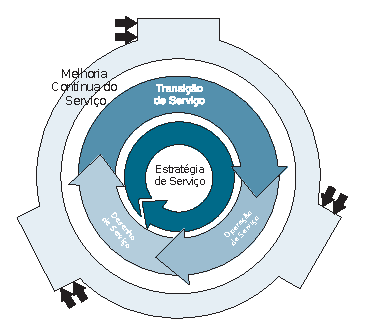
\includegraphics[width=.70\textwidth]{figuras/ciclo_itil.eps} 
  \caption{Ciclo de Vida de Serviços \acrshort{itil} v3 (Adaptada de \cite{servicestrategy}).}
  \label{fig-ciclo-de-vida-itil} 
\end{figure}

Cada fase deste ciclo é documentado através da produção de um livro, e cada um destes tem como objetivo fornecer um conjunto de boas práticas para uma das fases de implantação do \acrshort{itil} na organização \cite{servicestrategy, introductoryoverviewofitil, arraj2010itil}. Deve-se salientar que um princípio chave de cada uma das etapas do ciclo de vida de serviços é a entrega dos valores necessários para que seja possível o alcance dos objetivos de negócio da organização \cite{commerce2007official}.

\subsection*{Estratégia de Serviço (\textit{Service Strategy})}

\noindent A principal etapa do ciclo de vida de serviços é a Estratégia de Serviço, pois tem como característica o foco na entrega de valores necessários para o atendimento das necessidades do cliente e não apenas na entrega do produto \cite{introductoryoverviewofitil}. A Estratégia de Serviço pode ser definida como um conjunto de orientações de como projetar, desenvolver e implementar o gerenciamento de serviços sobre uma perspectiva de ativo estratégico \cite{itilimplementationfailure}. Seu objetivo está na definição da perspectiva, posição, planos e padrões que são necessários para que o prestador de serviço seja capaz de executar e atender os resultados que são esperados pela organização \cite{servicestrategy}.

Outra característica da Estratégia de Serviço está no fornecimento de orientação aos prestadores de serviços sobre a forma como os processos e as políticas de gerenciamento devem ser planejados, desenvolvidos e implantados ao decorrer do ciclo de vida dos serviços \cite{abreu2012implantando}. A execução da fase de Estratégia de Serviço promove as seguintes mudanças na organização \cite{servicestrategy}:

\begin{itemize}
    \item Um entendimento sobre o que é estratégia;
    \item Uma clara identificação e definição dos serviços que os clientes necessitam;
    \item A habilidade de definir como o valor é criado e distribuído;
    \item Identificar oportunidades para explorar e fornecer serviços;
    \item Um modelo claro de prestação de serviço que articula a forma como os serviços serão entregues e com qual propósito; e
    \item Processos que definem a estratégia da organização, quais serviços vão seguir a estratégia, em qual nível de demanda e os meios para garantir a existência de uma relação de trabalho entre o cliente e o provedor de serviços.
\end{itemize}

A Estratégia de Serviço é formada por três principais processos, sendo eles: Gerenciamento Financeiro de \acrshort{ti}, Gerenciamento do Portfólio de Serviços e Gerenciamento da Demanda \cite{abreu2012implantando}.

A etapa de gerenciamento financeiro consiste na gerência da parte de finanças do Portfólio de Serviços de \acrshort{ti} da organização de forma a oferecer o equilíbrio econômico necessário na execução dos serviços \cite{abreu2012implantando}. O processo de gerência financeira, por sua vez, tem como finalidade fornecer um nível adequado de recursos financeiros necessários para projetar, desenvolver e fornecer serviços de \acrshort{ti} que atendam às necessidades da organização \cite{introductoryoverviewofitil}. Uma gestão financeira rigorosa proporciona uma maior visibilidade operacional, percepção e tomada de decisões superiores para as organizações de \acrshort{ti} de forma a oferecer aos negócios da organização uma melhor percepção sobre o real valor dos serviços prestados\cite{commerce2007official}.

O Gerenciamento de Portfólio tem como objetivo garantir ao prestador de serviços de \acrshort{ti} uma combinação correta de serviços de forma a equilibrar os investimentos em \acrshort{ti} com a capacidade de atender os resultados de negócio \cite{introductoryoverviewofitil}. A etapa referente à gerência de portfólio visa, sobretudo, governar os investimentos da empresa na gerência de serviços adicionando valor ao negócio e estabelecendo duas categorias de serviços: os serviços de negócios e os serviços de \acrshort{ti} \cite{abreu2012implantando}.

No Gerenciamento de Demanda procura-se gerenciar de maneira síncrona os ciclos de produção de serviços e os ciclos de consumo dos serviços \cite{abreu2012implantando}. Esse processo é um aspecto crítico do gerenciamento de serviços, pois em casos de má administração das demandas é criado um sentimento de incerteza sobre a execução do serviço que se transforma em um grande fator de risco aos negócios da organização \cite{introductoryoverviewofitil}.

A Figura \ref{relacao-etapas-itil} apresenta a relação entre as etapas do ciclo de vida de serviços do \acrshort{itil}, na qual podemos constatar que a Estratégia de Serviço é o centro  do ciclo de vida de serviços, pois representa a principal fonte de requisitos para as demais etapas, já a Melhoria Contínua do Serviço está presente em todos os estágios por fornecer suporte às demais etapas através de medições e avaliações de desempenho sobre cada uma das etapas do ciclo de vida de serviços \cite{abreu2012implantando}.

\begin{figure}[!ht]
  \centering
  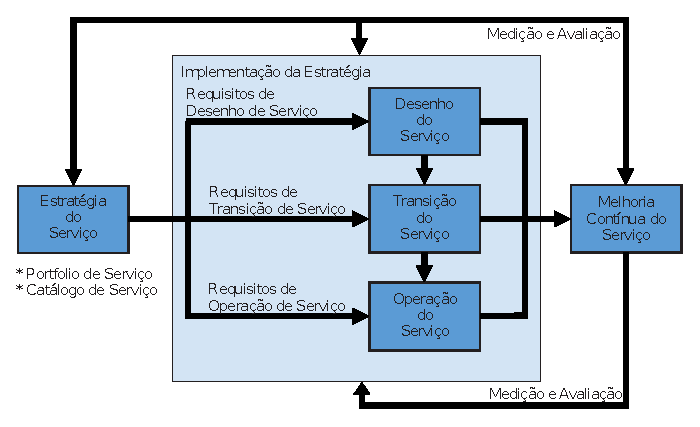
\includegraphics[width=.70\textwidth]{figuras/relacao-etapas-itil.eps} 
  \caption{Relação entre as etapas do Ciclo de Vida de Serviços (Adaptada de \cite{abreu2012implantando, servicestrategy}).}
  \label{relacao-etapas-itil} 
\end{figure}

\subsection*{Desenho de Serviço (\textit{Service Design})}

\noindent O Desenho de Serviço é um conjunto de orientações que objetiva a concepção e o desenvolvimento de serviços e gerenciamento de processos, com foco na concepção do serviço de \acrshort{ti} por meio de práticas de Governança de \acrshort{ti}, processos e políticas que têm como principal objetivo satisfazer as necessidades do cliente. Essa prática resulta em uma entrega de serviços com qualidade e um menor preço de produção \cite{itilimplementationfailure, servicedesign}.

Através dessa etapa é apresentada uma série de orientações sobre o planejamento e desenvolvimento do gerenciamento de serviços e processos almejando promover melhorias na entrega de valor aos clientes no decorrer do ciclo de serviços, além de fornecer um aspecto detalhado do gerenciamento do catálogo de serviços, de sua capacidade, continuidade, da segurança da informação, dentre outros \cite{abreu2012implantando}.

\noindent São objetivos do Desenho de Serviço \cite{servicedesign}:

\begin{itemize}
    \item Possibilitar com mais precisão a estimativa de custos, tempo, exigência e riscos associados com os recursos relacionados com a etapa de planejamento de serviços;
    \item Facilitar a criação de métodos de planejamento com facilidade tornando mais fácil de serem seguidas;
    \item Reduzir os atrasos causados pela necessidade de replanejamento dos serviços antes da conclusão da Transição de Serviço.
    \item Proporcionar melhoria no gerenciamento das expectativas das partes interessadas que inclui clientes, usuários, fornecedores, parceiros do projeto;
    \item Aumentar a confiança na entrega de serviços novos ou modificados; e
    \item Certificar que a criação de serviços novos ou modificados tenham fácil manutenção e baixo custo.
\end{itemize}

A etapa de Desenho de Serviço é composto por sete principais processos, são eles: Gerenciamento do Catálogo de Serviços, Gerenciamento do Nível de Serviço, Gerenciamento da Capacidade, Gerenciamento da Disponibilidade, Gerenciamento da Continuidade do Serviço, Gerenciamento da Segurança da Informação e Gerenciamento de Fornecedores \cite{abreu2012implantando}. A Figura \ref{relacao-desenho-servico} mostra uma visão geral dos processos da etapa de Desenho de Serviço, evidenciando a maneira como é feita a interligação entre os processos \cite{abreu2012implantando}.

O catálogo de serviços consiste em um banco de dados ou documento que estrutura todas as informações sobre os serviços de \acrshort{ti}, o que inclui informações sobre as entregas, preços, pontos de contatos e ordenação dos processos de solicitação dos serviços \cite{servicedesign}.

O Gerenciamento do Catálogo de Serviços fornece uma fonte central com informações sobre os serviços entregues pela organização prestadora de serviços de \acrshort{ti}, disponibilizando uma visão mais precisa e detalhada sobre quais são os serviços disponíveis oferecidos pela \acrshort{ti} \cite{introductoryoverviewofitil}. O Catálogo de Serviços tem duas subdivisões \cite{abreu2012implantando}:

\begin{itemize}
    \item Catálogo de Serviços de Negócio: engloba a visão do cliente sobre os serviços de \acrshort{ti}, além de proporcionar um melhor relacionamento deste com os processos e estruturas organizacionais do negócio; e
    \item Catálogo de Serviços Técnicos: oferece maiores detalhes técnicos de todos os serviços oferecidos ao cliente, detalhando como é o relacionamento do cliente com os serviços de suporte, itens de configurações e demais pormenores que são necessários para a execução do serviço prestado.
\end{itemize}

\begin{figure}[!h]
  \centering
  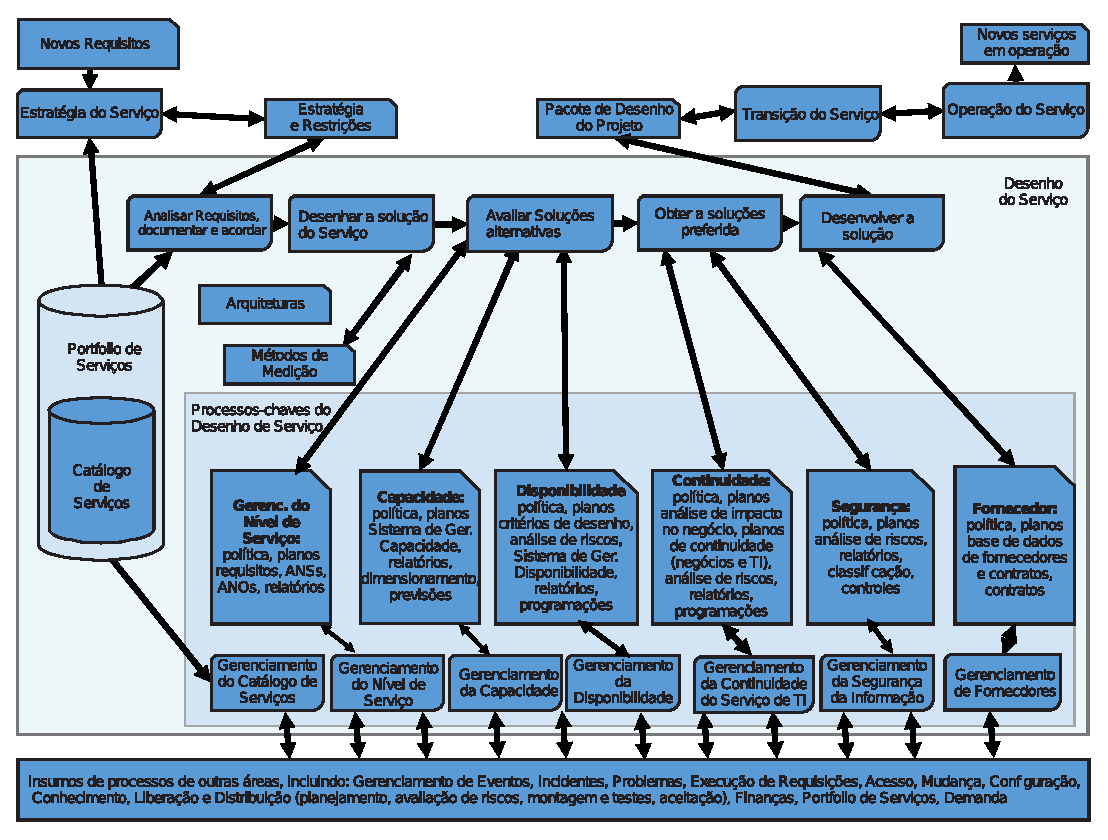
\includegraphics[width=1\textwidth]{figuras/desenho-servico.eps} 
  \caption{Visão geral dos processos do Desenho de Serviço (Adaptada de \cite{abreu2012implantando, servicedesign}).}
  \label{relacao-desenho-servico} 
\end{figure}

Outro item definido pelo Desenho de Serviço é o processo de \gls{slm_itil}, o \acrshort{slm_itil} é um documento utilizado pelos prestadores de serviços de \acrshort{ti} e clientes que visa proporcionar melhorias na qualidade dos serviços prestados pela \acrshort{ti} \cite{introductoryoverviewofitil}. Sua utilização tem como propósito a definição de um ciclo contínuo de atividades que envolvem o planejamento, coordenação, elaboração e estabelecimento de acordo e metas de desempenho através de um acordo de responsabilidade mútua entre os envolvidos \cite{abreu2012implantando}.

É papel do \acrshort{slm_itil} negociar, concordar e documentar as metas dos serviços de \acrshort{ti} verificando se estão adequadas com os negócios e com o \acrshort{sla}, sendo possível em sequência, iniciar a fase de monitoramento e produção de relatórios sobre as entregas dos serviços prestados \cite{introductoryoverviewofitil}. 

Desta maneira, observa-se que seu principal propósito é assegurar que todas as operações de serviços e seus desempenhos sejam medidos de forma consistente e profissional por toda a organização de \acrshort{ti}, de modo que os relatórios emitidos durante a execução dos serviços tenham como foco atender as necessidades de negócio do cliente \cite{introductoryoverviewofitil}.

É definido no processo de Gerenciamento da Capacidade questões que asseguram a capacidade da infraestrutura de \acrshort{ti} de absorver a crescente demanda de novos negócios requisitados pela organização, de forma que minimize os riscos e interrupções que possam ocorrer pelos prestadores de serviços da \acrshort{ti} \cite{abreu2012implantando}.

O fator de sucesso do processo em questão está na sua utilização durante a fase de planejamento de serviço, uma vez que o seu principal objetivo está na capacidade de fornecer um foco maior na gestão de problemas relacionados ao desempenho do tempo de resposta da \acrshort{ti} em atender as demandas de negócio da organização \cite{introductoryoverviewofitil}.

Um dos principais objetivos do Gerenciamento da Disponibilidade está em promover melhorias na disponibilidade dos serviços fornecidos pela \acrshort{ti}, de forma que as questões relacionadas a disponibilidade do serviço assegurem que os objetivos da organização sejam alcançados de forma custo efetiva \cite{introductoryoverviewofitil}. A preservação do nível de confiabilidade dos serviços de \acrshort{ti} é um fator crítico para que haja confiança sobre a disponibilidade dos serviços oferecidos pela \acrshort{ti}, uma boa execução do processo de gerenciamento de disponibilidade assegura que os riscos de interrupções dos serviços sejam minimizados através da utilização de abordagens de monitoramento das atividades físicas e de solução de incidentes que visam a melhoria contínua da organização de suporte \cite{abreu2012implantando}.

O Gerenciamento da Continuidade do Serviço por sua vez, visa assegurar que os serviços de \acrshort{ti} tenham os recursos necessários para sua continuação, como recursos de infraestrutura, manutenibilidade de serviços e o suporte técnico, e que estes estejam disponíveis sempre que houver necessidade de sua utilização. Isto sugere a existência de um tempo preestabelecido de resposta ao atendimento \cite{abreu2012implantando}.

Assim, o objetivo principal do gerenciamento de continuidade é manter a capacidade de recuperação dos serviços de \acrshort{ti} em corresponder as necessidades definidas na etapa de desenho dos serviços, tendo sempre como meta o cumprimento dos requisitos estabelecidos dentro dos prazos definidos \cite{introductoryoverviewofitil}.

É através do processo de Gerenciamento da Segurança da Informação que são definidos os processos relacionados a garantia da segurança das informações das organizações, utilizadas pelos serviços prestados pela \acrshort{ti}, assegurando a aplicação de políticas de segurança nos serviços de \textit{software} e de \textit{hardware} oferecidos pelos prestadores de serviços em todo o ciclo de vida dos serviços \cite{abreu2012implantando}. Sua proposta é alinhar a segurança da \acrshort{ti} com os negócios da organização, de forma que garanta que as políticas de segurança da informação sejam efetivamente aplicadas, são elas \cite{introductoryoverviewofitil}:

\begin{itemize}
    \item Garantia da disponibilidade e usabilidade da informação quando requisitada;
    \item Garantia da confidencialidade e integridade das informações através de uma política de níveis de permissões de leitura e escrita; e
    \item Garantia de uma transação confiável das informação comerciais.
\end{itemize}

No processo de Gerenciamento de Fornecedores são definidas formas que garantam que os provedores de serviços de \acrshort{ti} atendam às expectativas de negócio da organização, tendo como objetivo assegurar que os serviços sejam executados e atinjam as metas preestabelecidas nos contratos e acordos \cite{introductoryoverviewofitil}. Seu foco está em gerir fornecedores e contratos de forma que seja suprida as necessidades da organização, promovendo melhorias na transparência dos negócios desta e no retorno do valor investido \cite{abreu2012implantando}.

\subsection*{Transição de Serviço (\textit{Service Transition})}

\noindent O objetivo da fase de Transição de Serviço é garantir que serviços novos, modificados ou aposentados atendam às expectativas de negócios que estão documentadas na Estratégia de Serviço e Desenho de Serviço, fornecendo um conjunto de orientações para que ocorram melhorias e aperfeiçoamento das habilidades do prestador de serviços sobre como fazer transição e mudanças de seus serviços durante sua execução no ciclo de vida do \acrshort{itil} \cite{servicetransiction, itilimplementationfailure}. São objetivos da Transição de Serviço \cite{servicetransiction}:

\begin{itemize}
    \item Planejar e gerenciar alterações de serviços de forma eficiente e eficaz;
    \item Gerenciar riscos relacionados a serviços novos, alterados ou aposentados;
    \item Implantar com êxito novas versões dos serviços em ambientes suportados;
    \item Definir expectativas sobre o desempenho do uso de serviços novos ou alterados;
    \item Verificar se as alterações de serviços criam realmente o valor esperado para o negócio; e
    \item Fornecer informações sobre a qualidade dos serviços e bens de serviços.
\end{itemize}

A fase de Transição de Serviço é divido em seis principais processos, são eles: Gerenciamento de Mudanças, Gerenciamento de Ativos de Serviço e da Configuração, Gerenciamento da Liberação e Distribuição, Validação e Teste do Serviço, Avaliação e Gerenciamento do Conhecimento \cite{abreu2012implantando, servicetransiction}.

O processo de Gerenciamento de Mudanças visa minimizar o impacto causado pelas transformações provocadas durante a execução dos serviços, ela busca assegurar um tratamento sistemático e padronizado das possíveis mudanças que possam ocorrer no ambiente operacional da organização \cite{abreu2012implantando}. A gestão de mudanças tem como foco proporcionar um melhor controle em todo o ciclo de vida de serviços permitindo que sejam feitas alterações benéficas com um efeito mínimo de perturbação sobre a execução dos serviços prestados pela \acrshort{ti} \cite{introductoryoverviewofitil}.

O Gerenciamento de Ativos de Serviço e da Configuração é responsável por fazer a identificação dos registros e controle de verificação de ativos de itens de serviços de configuração, como componentes de \acrshort{ti}, itens de \textit{hardware}, \textit{software} e documentação associada aos serviços fornecidos pela \acrshort{ti} \cite{abreu2012implantando}. O processo procura fornecer apoio aos negócios fornecendo informações necessárias para gerenciar os demais serviços da etapa de ciclo de vida do \acrshort{itil}, o que contribui o sucesso em todas as etapas do ciclo de gerenciamento de serviços, proporcionando uma obtenção do máximo valor dos ativos de serviços \cite{introductoryoverviewofitil}.

O desenvolvimento do Gerenciamento da Liberação e Distribuição está centrado na gerência de um conjunto de mudanças sobre um serviço de \acrshort{ti}, sendo estas devidamente autorizadas, por exemplo, atividades de planejamento e configuração de itens de \textit{software} e \textit{hardware}, com o propósito de criar um conjunto de componentes finais para serem implantados em blocos no ambiente de produção \cite{abreu2012implantando}. Desse modo, seu propósito consiste em fornecer formas de planejamento da implantação dos serviços, assim como estratégias para programar o lançamento de novas funcionalidades de forma que novas modificações feitas não afetem o funcionamento de serviços já em produção \cite{introductoryoverviewofitil}.

A etapa de Validação e Teste do Serviço está relacionada com a garantia da qualidade de entrega de um serviço novo ou alterado, sendo feito testes para a validação do mesmo com o objetivo de garantir que seja entregue um serviço de acordo com o propósito definido na etapa de Desenho do mesmo \cite{abreu2012implantando}. Essa prática propicia a adequação dos serviços às especificações e necessidades de negócio, possibilitando uma maior confiança no lançamento de novas atividade e garantindo a entrega de valor ao cliente \cite{introductoryoverviewofitil}.

O processo de Avaliação é responsável pela criação de formas padronizadas para  avaliar o desempenho que uma mudança pode proporcionar nos serviços já em execução mantidas pela \acrshort{ti} em confronto com as metas estipuladas, registrando e gerenciando os desvios encontrados \cite{abreu2012implantando}. O principal resultado obtido, dessa maneira, está na capacidade de geração de relatórios analíticos aos prestadores de serviços de \acrshort{ti} que auxiliarão a equipe responsável a obter uma visão geral sobre quais são as possíveis mudanças a serem realizadas nos processos do \acrshort{itil} para que ocorra uma melhoria na entrega de seus serviços \cite{introductoryoverviewofitil}.

O gerenciamento do conhecimento procura certificar que as informações corretas sejam entregues de forma apropriada para uma pessoa que tenha habilidades para atuar na atividade no tempo esperado, além de informar um conjunto de conhecimentos tais como a experiência de equipe, requisitos, habilidades, as expectativas dos fornecedores e parceiros e histórico de informações \cite{abreu2012implantando}. Sua principal proposta é gerir o conhecimento de forma a partilhar perspectivas, ideias, experiências e informações \cite{introductoryoverviewofitil}

\subsection*{Operação de Serviço (\textit{Service Operation})}

\noindent Operação de Serviço inclui orientações para a obtenção de eficácia na entrega e suporte de serviços de forma a assegurar o valor da entrega do serviço ao cliente. Esta fase configura-se como uma das mais críticas do ciclo de vida de serviços do \acrshort{itil}, pois mesmo que tenha um bom planejamento e implementação dos processo, todo o trabalho será nulo caso a organização não tenha uma cultura de monitoramento de informações como desempenho, avaliação de métricas e a coleta de dados operacionais \cite{serviceoperation, itilimplementationfailure}. São objetivos da etapa de Operação de Serviço \cite{serviceoperation}:

\begin{itemize}
    \item Manter a satisfação e confiança nos negócios da \acrshort{ti} através da entrega eficaz e eficiente dos serviços, além de fornecer suporte a eles;
    \item Minimizar o impacto de interrupções de serviços em atividades do dia-a-dia; e
    \item Certificar que os serviços de \acrshort{ti} sejam prestados apenas a setores autorizados.
\end{itemize}

A etapa de Operação de Serviço é dividida em um conjunto de cinco processos, são eles: Gerenciamento de Eventos, Gerenciamento de Incidentes, Execução de Requisições, Gerenciamento de Problemas e Gerenciamento do Acesso \cite{serviceoperation, abreu2012implantando}. A Figura \ref{relacao-processos-service-operation} apresenta os processos envolvidos na etapa de operação de serviço \cite{abreu2012implantando}.

\begin{figure}[!h]
  \centering
  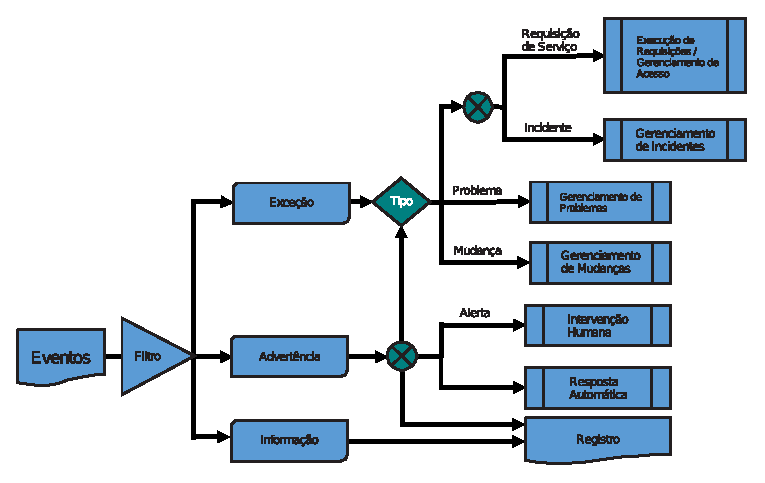
\includegraphics[width=.80\textwidth]{figuras/processos-service-operation.eps} 
  \caption{Visão geral dos processos do Operação de Serviço (Adaptada de \cite{abreu2012implantando, serviceoperation}).}
  \label{relacao-processos-service-operation} 
\end{figure}

O Gerenciamento de Eventos propõe a promoção de uma monitoria de todos os eventos que ocorrem na infraestrutura da \acrshort{ti}, tendo como intuito proporcionar a normalidade das operações do serviço \cite{abreu2012implantando}. Um evento pode indicar que algo não está funcionando corretamente, e nesse passo é necessária a criação de uma política de monitoramento de processos com o objetivo de apontar quais atividades estão dentro da normalidade e identificar que estejam atrapalhando o funcionamento normal de um determinado conjunto de serviços \cite{introductoryoverviewofitil}. 

Através do processo de gerenciamento de eventos busca-se promover melhorias no seu gerenciamento durante a execução no ciclo de vida de serviços, concentrando-se na geração e detecção de notificações significativas sobre eventuais problemas \cite{introductoryoverviewofitil}.

No Gerenciamento de Incidentes espera-se alcançar uma restauração da normalidade da operação de um serviço em um menor tempo possível, minimizando os impactos gerados nos negócios devido a ocorrência de eventuais incidentes, e focando na entrega de valor aos clientes dentro dos padrões acordados \cite{abreu2012implantando}. No entanto, incidentes são frequentemente detectados e reportados por meio da utilização de ferramentas de monitoramento ou através da reclamação feita diretamente na central de atendimento. Após feito o levantamento dos incidentes eles são catalogados e ordenados de acordo com sua prioridade e direcionados de acordo a sua necessidade de correção ao setor responsável. \cite{introductoryoverviewofitil}.

A Execução de Requisições define a forma como devem ser tratadas as requisições realizadas pelos usuários dos serviços de \acrshort{ti}, sendo elas originadas
de uma solicitação de serviço ou de uma simples solicitação de informação\cite{abreu2012implantando}.

A principal finalidade do processo de execução de requisições está em permitir que usuários tenham acesso às informações sobre os serviços prestados criando um canal de comunicação que torna possível fazer elogios ou reclamações sobre eventuais problemas com os serviços fornecidos pela \acrshort{ti} \cite{introductoryoverviewofitil}.

O método referente ao Gerenciamento de Problemas tem como propósito minimizar os impactos adversos que os incidentes causam para os negócios, de forma a proporcionar melhorias nas estratégias adotadas para a prevenção de incidentes \cite{abreu2012implantando}. As adversidades detectadas são classificadas de maneira semelhante ao gerenciamento de incidentes, tendo como característica principal a busca das causas do problema \cite{introductoryoverviewofitil}. Para solução deste é feito um levantamento de propostas contendo soluções alternativas \cite{introductoryoverviewofitil, serviceoperation}.

O Gerenciamento do Acesso, como o nome sugere, é responsável pelo controle de acesso do usuário, restringindo através de autorizações a possibilidade de alcance a informações e serviços, o que torna o processo mais seguro \cite{abreu2012implantando}.

O processo de Gerenciamento do Acesso visa ajudar o gerenciamento da confidencialidade, disponibilidade, integridade dos dados e propriedade intelectual das informações presentes no sistema \cite{introductoryoverviewofitil}. Ele inclui a verificação da identidade do usuário e suas restrições de acesso aos serviços, além de garantir que mudanças de permissões sejam feitas caso haja a necessidade \cite{introductoryoverviewofitil}.

\subsection*{Melhoria Contínua do Serviço (\textit{Continual Service Improvement})}

\noindent Um dos principais objetivos da Melhoria Contínua do Serviço está no alinhamento dos serviços de \acrshort{ti} com as necessidades de negócio da organização através da identificação e implementação de aperfeiçoamentos nos serviços prestados pela \acrshort{ti}. Tais mudanças são feitas através de uma melhor abordagem do ciclo de vida a fim de apoiar as demais etapas do mesmo, como a Estratégia de Serviço, Desenho de Serviço, Transição de Serviço e Operação de Serviço \cite{continualserviceimprovement}.

A Melhoria Contínua do Serviço serve como um guia que contém orientações de como criar e manter valor para o cliente através de um conjunto de melhorias no planejamento e na introdução de novos serviços, combinando princípios, práticas e métodos de aperfeiçoamento da qualidade da gestão dos serviços de \acrshort{ti} \cite{itilimplementationfailure}. São objetivos do Melhoria Contínua do Serviço \cite{continualserviceimprovement}:

\begin{itemize}
    \item Revisar, analisar além de fazer recomendações de mudanças para melhorias nos processos do ciclo de vida como o Estratégia de Serviço, Desenho de Serviço, Transição de Serviço, Operação de Serviço e até mesmo da própria Melhoria Contínua do Serviço;
    \item Revisar e analisar o nível de realização do serviço;
    \item Identificar e implementar atividades específicas com o objetivo de melhorar a qualidade dos serviços de \acrshort{ti}; e
    \item Melhorar a eficácia do custo de entrega dos serviços de \acrshort{ti} sem que seja necessário sacrificar a satisfação do cliente.
\end{itemize}

A Figura \ref{relacao-processos-csi} mostra os conceitos envolvidos no estágio de Melhoria Contínua do Serviço cuja base é composta por dois principais processos, sendo eles o Relato do Serviço e Medição do Serviço.

\begin{figure}[!h]
  \centering
  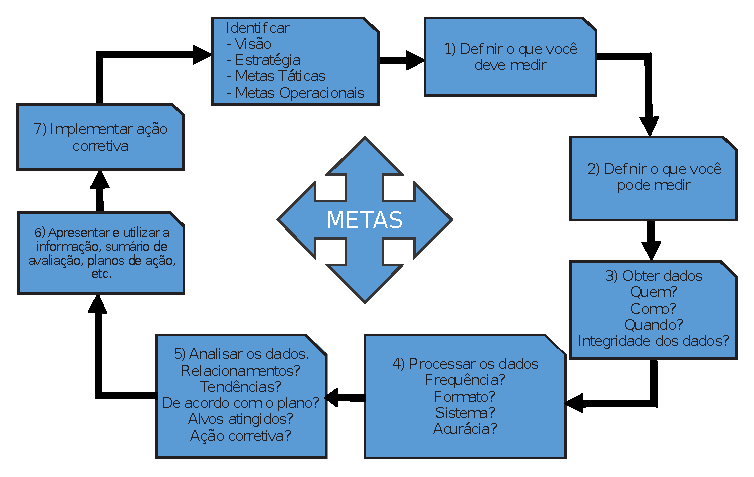
\includegraphics[width=.70\textwidth]{figuras/processos-ci.eps} 
  \caption{Visão geral dos processos do Melhoria Contínua do Serviço (Adaptada de \cite{abreu2012implantando, continualserviceimprovement}).}
  \label{relacao-processos-csi} 
\end{figure}

O processo de Relato do Serviço é a formalização de um conjunto de relatórios que contém informações coletadas a partir do monitoramento das estregas de serviços, a identificação de dados como definição do objetivo do serviço relatado e do público-alvo \cite{abreu2012implantando}.

A utilização de um relatório contendo apenas a adesão ou não da \acrshort{sla} não é autossuficiente, assim, é de grande importância que os prestadores de serviços de \acrshort{ti} possam criar uma abordagem acionável para a elaboração dos relatórios de serviços, sendo necessário que contenha informações que responda as seguintes perguntas \cite{introductoryoverviewofitil}: 

\begin{itemize}
    \item Porque aconteceu determinados eventos?
    \item Quem realizou tal ação?
    \item Como garantir que antigos incidentes não impactem novamente o serviço?
    \item Como melhorar a prestação de serviço?
\end{itemize}

A Medição do Serviço foca no fornecimento de uma visão completa e orientada sobre a integração dos serviços aos valores de negócios da organização. Para que haja tal modelo de medição é necessário que sejam estabelecidos diferentes níveis de avaliações para sua apreciação através dos relatórios \cite{abreu2012implantando}. Existem três tipos de métricas que uma organização necessita para recolher e apoiar as atividades da etapa de Melhoria Contínua do Serviço, são elas \cite{introductoryoverviewofitil}: 

\begin{itemize}
    \item Métricas de Tecnologia, que em muitos casos está diretamente associada a métricas de componentes e base de aplicações, tais como desempenho e disponibilidade;
    \item Métricas de Processo que está diretamente ligada aos indicadores chave de desempenho e métricas de atividade; e
    \item Métricas de Serviços que demostram resultados de serviços fim-a-fim, onde métricas de componentes e tecnologia são utilizadas para calcular as métricas de serviço.
\end{itemize}

\section{Especificação de Requisito de \textit{Software}}

\noindent É um grande desafio para os desenvolvedor o ato de saber analisar e projetar \textit{software} de forma a satisfazer os requisitos que os clientes esperam encontrar no produto \cite{pressmanengenharia}. Assim, um bom planejamento e definição dos requisitos para a construção do \textit{software} proporciona um melhor entendimento do projeto, fornecendo aos desenvolvedores e clientes um documento claro com informações a respeito dos requisitos necessários para o desenvolvimento do produto especificado \cite{pressmanengenharia}. 
Especificações como a \gls{ieee} 830 \cite{ieee1998ieee} fornecem um conjunto de informações contendo descrições importantes para o desenvolvimento do \textit{software} em questão, como levantamento de Requisitos Funcionais, Requisitos não Funcionais além de uma descrição detalhada do serviço projetado.

A documentação \acrshort{ieee} 830/98 é definida pela \acrshort{ieee} \textit{Standards}, onde são descritas informações com as melhores práticas para especificação de \textit{software} \cite{ieee1998ieee}.  Sua finalidade está em fornecer diversos atributos que são necessários para o desenvolvimento e implantação de serviços de \textit{software}. O uso do \gls{srs} tem como principal benefícios \cite{ieee1998ieee}:

\begin{itemize}
    \item Estabelecer bases de acordo entre os clientes com os fornecedores do serviço de forma a definir o que \textit{software} deve fazer;
    \item Promover uma redução do esforço para desenvolvimento do projeto, pois a \acrshort{srs} define todos os requisitos necessários para o desenvolvimento e implantação do \textit{software}; e
    \item Proporcionar uma melhoria na estimativa de entrega das atividades e etapas de finalização do \textit{software}.
\end{itemize}

\section{Metodologia de Desenvolvimento Ágil}

\noindent A adoção de métodos ágeis de desenvolvimento de \textit{software} tem sido utilizada por diversas empresas de desenvolvimento. A adesão de tais práticas visa, sobretudo, tornar o planejamento e execução de projetos mais versáteis e adaptáveis à realidade de mudanças diárias de requisitos de \textit{software} \cite{pressmanengenharia, rubin2012essential}.

\subsection{Manifesto Ágil}

\noindent O termo agilidade surgiu no ano de 2001 por Kent Beck e mais 16 desenvolvedores renomados da área de \textit{software}, dando origem ao termo ``\textit{Agile Alliance}'', culminando na assinatura de um manifesto a favor do desenvolvimento ágil de \textit{software} \cite{pressmanengenharia}. O Manifesto Ágil é um movimento precursor do surgimento dos métodos ágeis de desenvolvimento que tem como princípio a busca por maneiras de implementar um \textit{software} de forma ágil. São princípios fundamentais do manifesto ágil \cite{agilemanifesto}:

\begin{itemize}
    \item \textbf{Indivíduos e interações} mais que processos e ferramentas;
    \item \textbf{\textit{Software} em funcionamento} mais que documentação abrangente;
    \item \textbf{Colaboração com o cliente} mais que negociação de contratos; e
    \item\textbf{Responder a mudanças} mais que seguir um plano.
\end{itemize}

Beck \cite{agilemanifesto} afirma que mesmo que se tenha um maior valor nos itens à direita, os princípios do manifesto ágil focam mais nos itens da esquerda.

\subsection{Metodologia \textit{Scrum}}

\noindent O \textit{Scrum} é uma metodologia de desenvolvimento ágil de \textit{software} criado inicialmente por Jeff Sutherland no início de 1990 \cite{pressmanengenharia}. Uma característica presente nele é o fato de sua ideologia seguir também os princípios presentes no manifesto ágil, tendo como propósito orientar as atividades estruturais de desenvolvimento de \textit{software}, como o levantamento de requisitos, análise dos processos, planejamento do projeto e métodos de evolução e entregas de \textit{software} \cite{pressmanengenharia}.

A Figura \ref{fig-ciclo-scrum} mostra o ciclo de atividades da metodologia \textit{Scrum} de desenvolvimento ágil, onde diversos termos são utilizados para caracterizar as etapas presentes na metodologia, como o \textit{Product Backlog}, \textit{Sprint Backlog}, \textit{Daily Scrum Meeting} e o \textit{Potentially Shippable Product Increment} \cite{pressmanengenharia}.

\begin{figure}[!h]
  \centering
  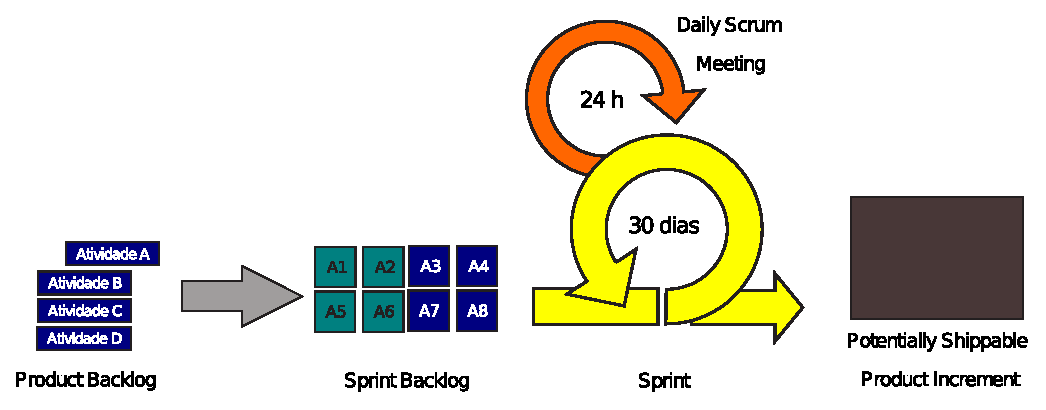
\includegraphics[width=1\textwidth]{figuras/scrum_ciclo.eps} 
  \caption{Ciclo de atividades da metodologia \textit{Scrum} (Adaptada de \cite{pressmanengenharia}).}
  \label{fig-ciclo-scrum} 
\end{figure}

Cada fase presente no ciclo de atividades do \textit{Scrum} tem um papel importante para o seu sucesso na implantação dos serviços de \textit{software}. Sua divisão consiste em \textit{Sprints} que são ciclos de atividades catalogadas pelo \textit{Product Backlog}, sendo dever do \textit{Product Owner} definir quais atividades deverão ser executadas primeiro no projeto através da etapa de \textit{Sprint Planning Meeting} \cite{rubin2012essential}.

O \textit{Scrum} é um aprimoramento da abordagem interativa e incremental para a entrega de \textit{software} orientado a objetos, inicialmente a metodologia foi documentada por Pittman mas posteriormente seus conceitos foram expandidos por Booch \cite{schwaber1997scrum}. De forma geral o \textit{Scrum} é uma metodologia para o gerenciamento de melhorias contínuas na manutenção de um projeto de \textit{software} já existente ou em desenvolvimento \cite{schwaber1997scrum}.

\subsection*{\textit{Product Backlog}}

\noindent Outra característica desta metodologia é a execução da tarefa com maior risco ser feita primeiro, ficando para o \textit{Product Owner} o dever de gerenciar quais tarefas devem ser priorizadas primeiro, influenciando assim todo o andamento da execução das atividades no \textit{Scrum} \cite{rubin2012essential}. A Figura \ref{product-backlog} mostra como é organizada as tarefas em um ordenamento de prioridades de execução (da mais alta prioridade para o de menor prioridade), sendo a definição das prioridades das atividades conhecida como \textit{Product Backlog} \cite{rubin2012essential}.

\begin{figure}[!h]
  \centering
  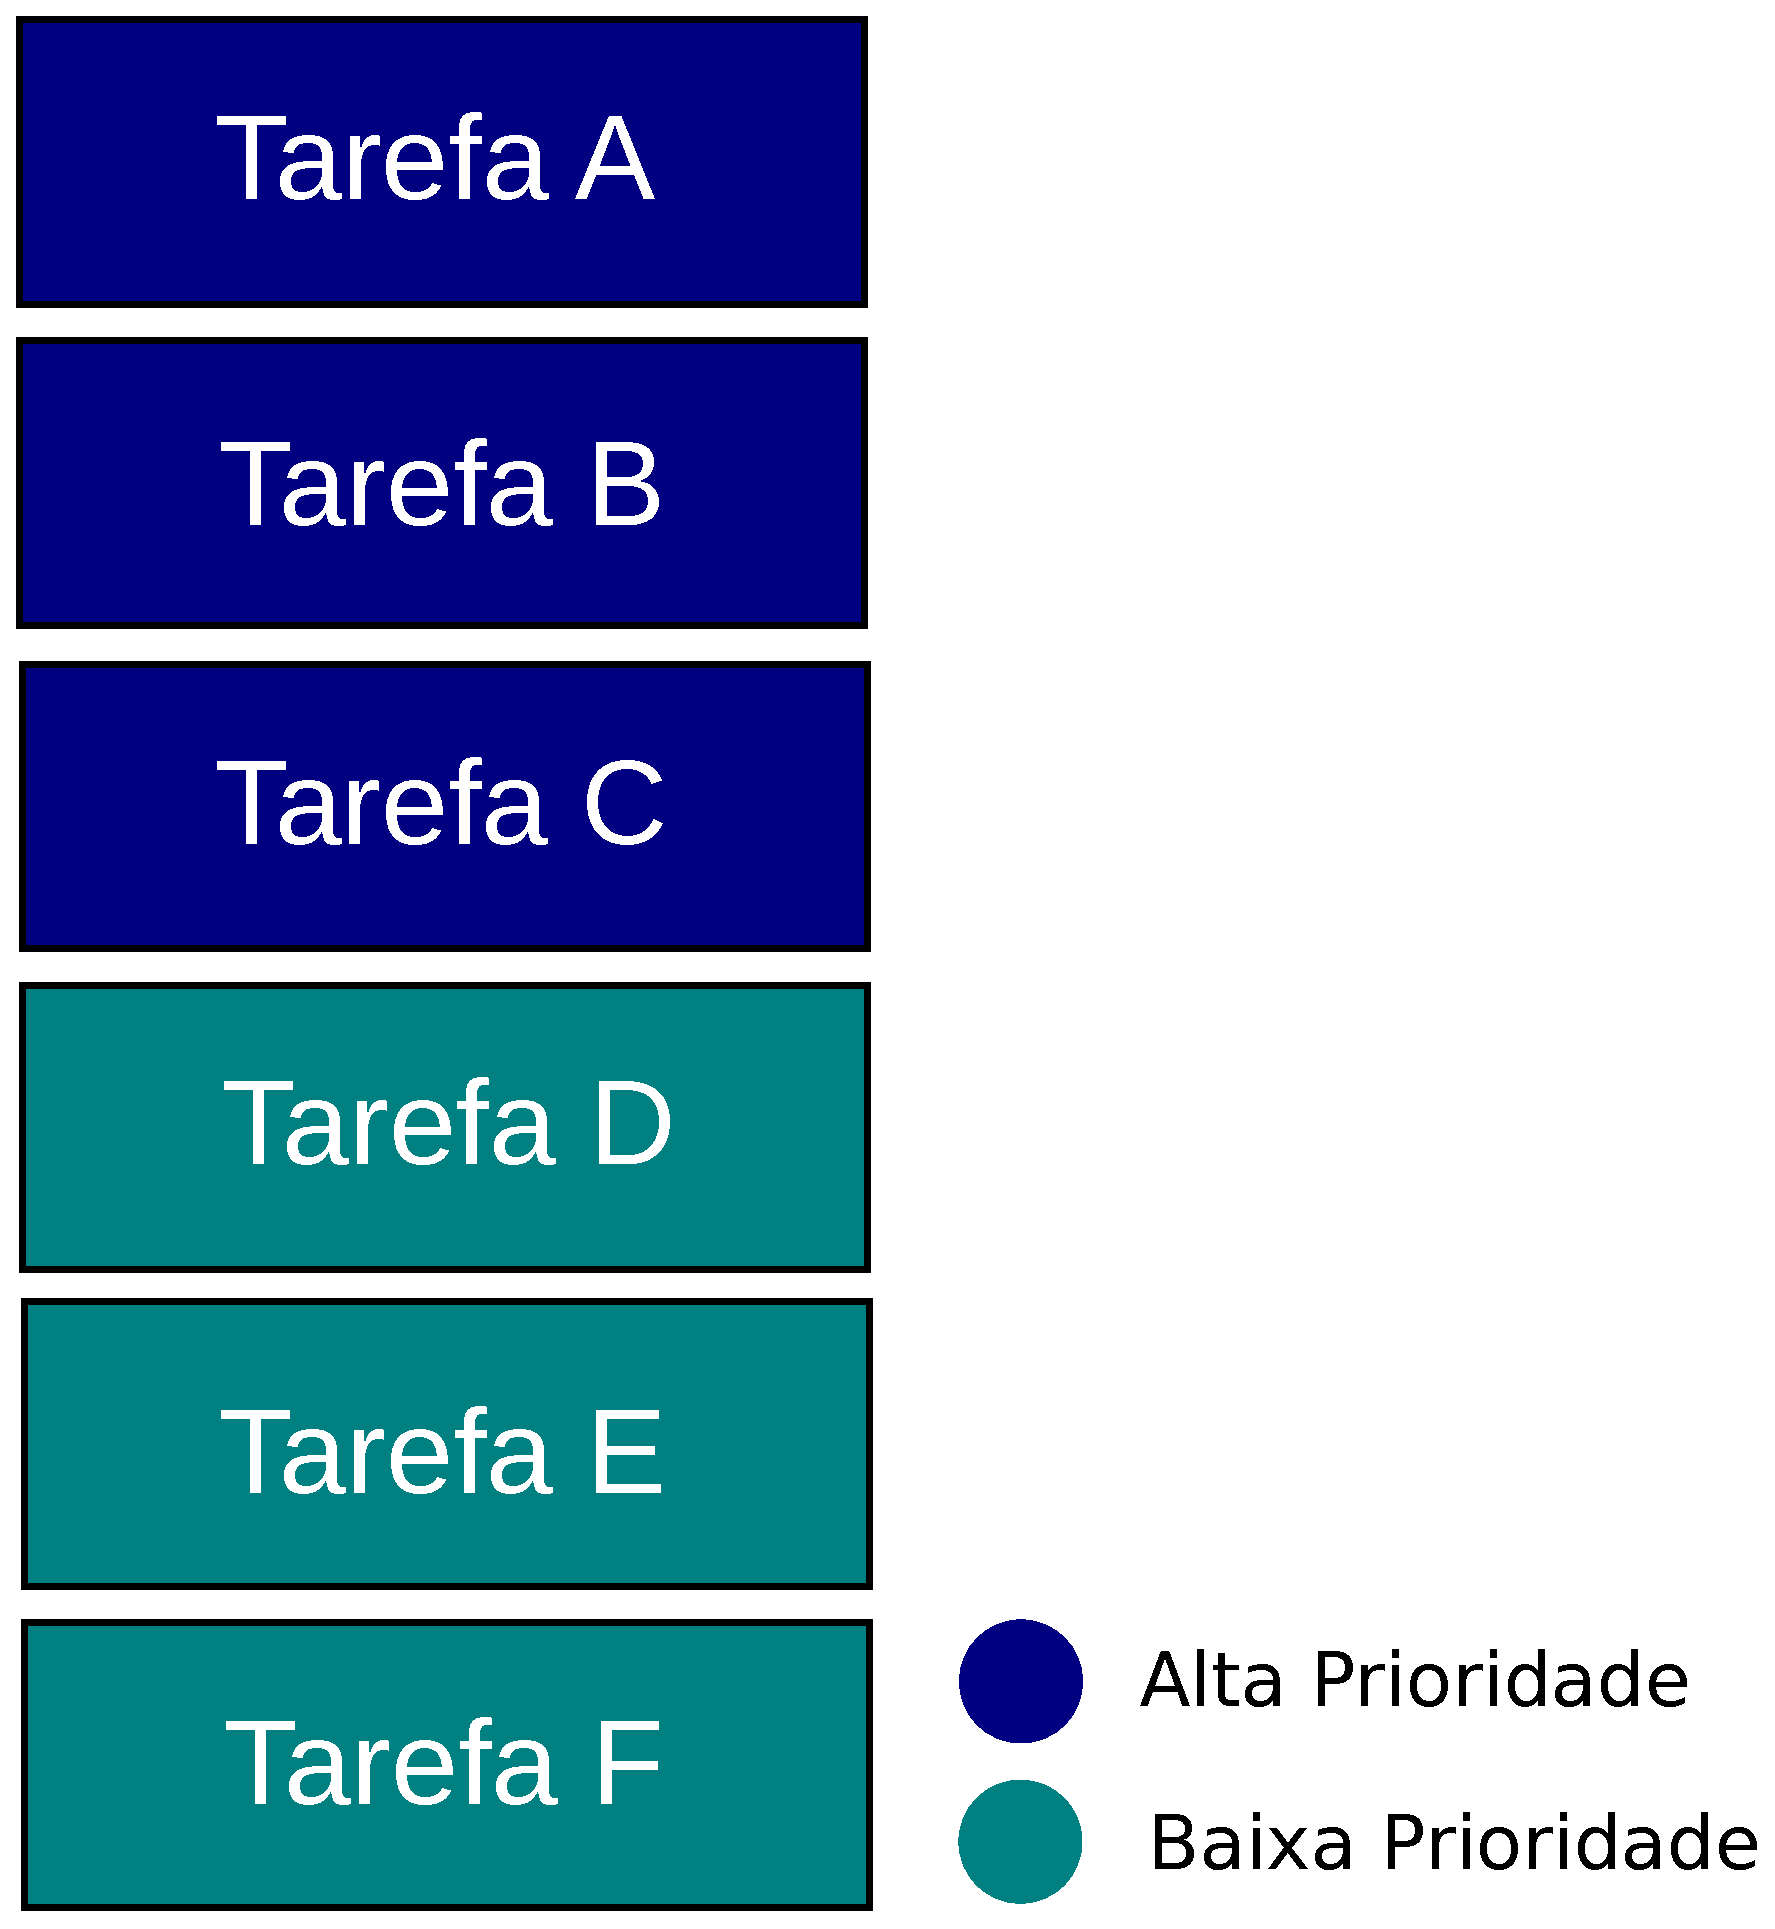
\includegraphics[width=.40\textwidth]{figuras/product_backlog3.eps} 
  \caption{Fase de \textit{Product Backlog} do \textit{Scrum} (Adaptada de \cite{rubin2012essential}).}
  \label{product-backlog} 
\end{figure}

O \textit{Product Backlog} consiste em uma pilha de atividades a serem realizadas pela equipe \textit{Scrum}, em que cada uma de atividade contém seu grau prioridade de execução o que influencia o ordenamento das tarefas a serem executadas \cite{rubin2012essential}.

\subsection*{\textit{Sprint Backlog}}

\noindent O \textit{Sprint Backlog} é uma fase do \textit{Scrum} onde as atividades são catalogadas e priorizadas pelo \textit{Product Backlog} e em sequência são agrupadas em forma de \textit{Sprints} de atividades, que tem como característica um conjunto de atividades prioritárias a serem realizadas pela equipe \textit{Scrum} \cite{pressmanengenharia, rubin2012essential}.

A Figura \ref{sprint-backlog} mostra o processo de definição do \textit{Sprint Backlog}, sendo cada atividade presente no \textit{Product Backlog} subdividida no \textit{Sprint Planning} através da criação de subconjuntos de atividades contendo as tarefas mais importantes definidas inicialmente pelo \textit{Product Owner} \cite{rubin2012essential}.

\begin{figure}[!h]
  \centering
  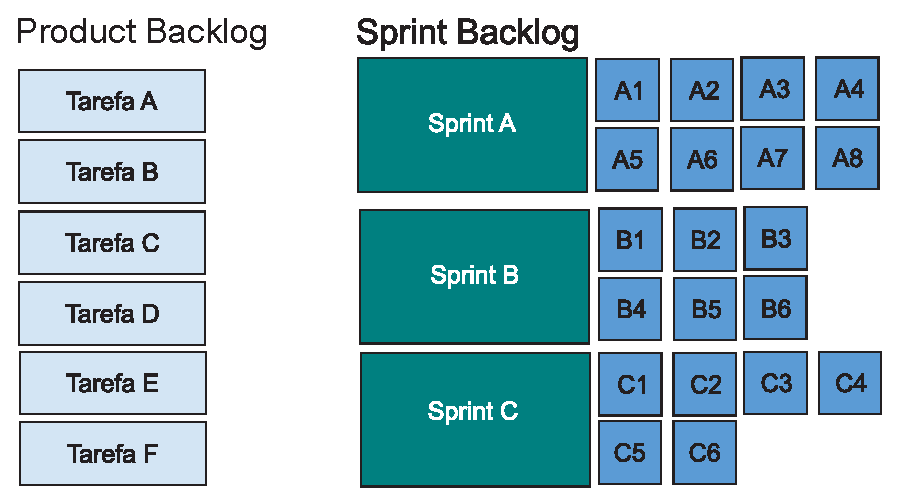
\includegraphics[width=.70\textwidth]{figuras/sprint-backlog.eps} 
  \caption{Fase de criação do \textit{Sprint Backlog} (Adaptada de \cite{rubin2012essential}).}
  \label{sprint-backlog} 
\end{figure}

\subsection*{\textit{Daily Scrum Meeting}}

\noindent O processo do \textit{Daily Scrum Meeting} visa criar reuniões diárias com duração de 15 minutos com os envolvidos no projeto, sendo dever do \textit{Scrum Master} auxiliar o andamento do projeto e organizar as reuniões de forma que seja feita analise do progresso da equipe frente as metas estabelecidas pelo \textit{Sprint} \cite{rubin2012essential}. Uma característica presente nestas reuniões é que os envolvidos permanecem em pé, com a finalidade de tornar as reuniões rápidas e objetivas. A cada reunião todos os membros da equipe respondem diariamente as seguintes perguntas feitas pelo \textit{Scrum Master} \cite{pressmanengenharia}:

\begin{itemize}
    \item O que você realizou desde a última reunião de equipe?
    \item Quais obstáculos está encontrando?
    \item O que você planeja realizar até a próxima reunião da equipe?
\end{itemize}

Outro dever do \textit{Scrum Master} é avaliar cada uma das respostas dadas pelos membros da equipe \textit{Scrum} e procurarventender e planejar novas formas para solucionar os problemas que foram catalogados durante aplicação do questionário \cite{pressmanengenharia, rubin2012essential}.

\subsection*{\textit{Potentially Shippable Product Increment}}

\noindent A fase de \textit{Potentially Shippable Product Increment} é o resultado das execuções das tarefas definidas no \textit{Sprint Planning} que resultaram em um estado de confiança de entrega de novas funcionalidades previstas no \textit{Sprint} \cite{rubin2012essential}.

O conceito de finalização do \textit{Sprint} depende muito dos objetivos que a equipe \textit{Scrum} deseja alcançar. Em alguns casos é decidido pela equipe que seja feito uma entrega parcial das atividades previstas no \textit{Sprint} com o propósito de reunir um conjunto de \textit{feedback} do cliente, que servirá de guia para a equipe contendo informações que os auxiliarão a identificar se as atividades entregues pela equipe estão realmente caminhando em direção ao objetivo desejado \cite{rubin2012essential}.

% ----------------------------------------------------------------------------------------------------- %
% Estado da Arte
% ----------------------------------------------------------------------------------------------------- %

%% ------------------------------------------------------------------------- %%
\chapter{Trabalhos Relacionados}

\noindent Neste capítulo serão apresentadas as principais ferramentas para abertura e encaminhamento de solicitação de ordem de serviço atualmente em produção, apontando suas principais características e pontos positivos além de expor as limitações encontradas. Em sequência, será apresentado uma visão geral sobre os mais recentes casos de estudo da aplicação do \acrshort{itil} na literatura, expondo os diversos benefícios de sua adoção.

\section{Aplicativos}

\noindent Atualmente, estão disponíveis diversas aplicações \textit{web} e \textit{mobile} no mercado que resolvem o problema de gerenciamento de ordens de serviço. No município de Palmas está em execução o aplicativo Alô Pequi \cite{alo_pequi}, inciativa da prefeitura de Palmas que possui como objetivo atender a necessidade do cidadão palmense em apontar os problemas de infraestrutura da cidade. No país existem diversas soluções para o problema mas a que se destaca de maneira acentuada é a plataforma Colab \cite{colab} pois contém aproximadamente mais de 50 mil \textit{downloads} na plataforma de aplicativos \textit{Google Play}. Seu diferencial está no modelo de rede social de colaboração como proposta do aplicativo. As próximas seções trazem uma visão geral das soluções atuais, onde será explicado as principais funcionalidades de cada aplicativo além de apontar os pontos positivos e negativos encontrado nos sistemas.

\subsection{Alô Pequi}

\noindent O aplicativo Alô Pequi é um \textit{software} utilizado para gestão de manutenção de serviços da prefeitura municipal da cidade de Palmas. Seu funcionamento consiste no modelo de abertura de solicitações de ordens de serviço através de um aplicativo móvel para as plataformas \textit{Android} e \acrshort{ios} aliado a uma central de atendimento para o encaminhamento dos chamados.

A Figura \ref{alo-pequi} mostra a tela inicial do aplicativo. O sistema consiste em uma ferramenta de envio de formulário onde são coletadas informações como a classificação do problema, observação, localização, data da solicitação e o envio de uma foto contendo o problema em questão.

\begin{figure}[!h]
\centering
    \begin{tabular}{cc}
     \includegraphics[width=.40\textwidth]{figuras/login_alopequi.png}  &   \includegraphics[width=.40\textwidth]{figuras/tela-inicial-alo-pequi.png} 
    \end{tabular}
    \caption{Tela inicial do aplicativo Alô Pequi (Adaptada de \cite{alo_pequi}).}
    \label{alo-pequi}
\end{figure}

Ao utilizar o aplicativo foram constatados diversos pontos positivos e negativos com respeito a usabilidade do sistema, abaixo são relatadas as experiências obtidas com o uso deste:

\subsection*{Pontos Positivos}

\begin{itemize}
    \item Aplicativo muti-plataforma pois utiliza o modelo híbrido de desenvolvimento;
    \item Detecção automática do local do problema pela localização do \acrshort{gps};
    \item Possibilidade de envio de foto do problema; e
    \item Acompanhamento do andamento do chamado.
\end{itemize}

\subsection*{Pontos Negativos}

\begin{itemize}
    \item Aplicativo apresenta lentidão por conta do seu modelo híbrido de desenvolvimento;
    \item Falta a opção de selecionar o local manualmente no mapa;
    \item Falhas na localização pelo \acrshort{gps}; e
    \item Interface muito simples e com poucas funcionalidades.
\end{itemize}

\subsection{Colab}

\noindent O aplicativo Colab é uma rede social que consiste em um sistema de colaboração sobre os problemas de infraestrutura de vários municípios do país, sua utilização atualmente está sendo feita pelas prefeituras de Niterói, Curitiba, Porto Alegre, Santos dentre outras. Existe a possibilidade de uso em qualquer cidade do país mas as ocorrências feitas pelo aplicativo não serão encaminhadas para as prefeituras que não estejam vinculadas à plataforma.

A Figura \ref{colab-app} mostra a tela inicial do aplicativo em que constata-se, pelo fato do sistema se basear no conceito de redes sociais, assim como o \textit{Facebook}\footnote{Facebook: http://www.facebook.com}, algumas características foram herdadas como: compartilhamento da solicitação feita por usuários da região, botão apoiar e opção de comentário.

\begin{figure}[!h]
\centering
    \begin{tabular}{cc}
     \includegraphics[width=.40\textwidth]{figuras/colab_start.png}  &   \includegraphics[width=.40\textwidth]{figuras/tela-inicial-colab-re.png} 
    \end{tabular}
    \caption{Tela inicial do aplicativo Colab (Adaptada de \cite{colab}).}
    \label{colab-app}
\end{figure}

Ao utilizar o aplicativo foram observados diversos pontos positivos e negativos com relação à usabilidade do sistema que serão relatados abaixo:

\subsection*{Pontos Positivos}

\begin{itemize}
    \item Padrão de rede social que proporciona um modelo melhor de colaboração;
    \item Opção ``apoiar problema relatado'';
    \item Utilização do \textit{Google Maps} para mostrar uma visão geral dos problemas da cidade;
    \item Disponibilidade de uma opção \textit{web} para o sistema do aplicativo; e
    \item Compartilhamento da reclamação com outras redes sociais.
\end{itemize}

\subsection*{Pontos Negativos}

\begin{itemize}
    \item Falta de moderação das reclamações postadas;
    \item Problemas com \textit{Spam};
    \item Falta de uma opção manual de escolha do local pelo mapa; e
    \item Cadastro feito apenas através de conta na rede social \textit{Facebook}.
\end{itemize}

\subsection{Vigilante App}

\noindent O aplicativo Vigilante App \cite{vigilante_app} é uma rede social colaborativa que visa tornar as informações sobre a cidade mais acessível aos cidadãos, proporcionando uma rede colaborativa de usuários para o compartilhamento de informações como o monitoramento de ocorrências, publicação de problemas com a infraestrutura da cidade dentre outros. A Figura \ref{vigilante-app} mostra a tela inicial do aplicativo.

\begin{figure}[!h]
\centering
    \begin{tabular}{cc}
     \includegraphics[width=.40\textwidth]{figuras/start_vigilante_app.png}  &   \includegraphics[width=.40\textwidth]{figuras/maps_vigilante.png} 
    \end{tabular}
    \caption{Tela inicial do aplicativo Vigilante App (Adaptada de \cite{vigilante_app}).}
    \label{vigilante-app}
\end{figure}

O sistema atualmente se encontra em fase beta de implantação, mas diversos recursos já estão disponíveis no aplicativo como denúncia de crimes, denúncia de problema infraestruturas como vazamento de água, esgoto e buracos em ruas. Uma característica importante do aplicativo é sua utilização estar voltada totalmente a visualização do mapa da cidade, onde é mostrado uma visão geral sobre os problemas encontrados na cidade. Ao utilizar o aplicativo foram constatados alguns pontos positivos e negativos levando em consideração à facilidade de uso do sistema, abaixo são relatados os pontos identificados:

\subsection*{Pontos Positivos}

\begin{itemize}
    \item Visualização das ocorrências em forma de mapa;
    \item Possibilidade de localização através do \acrshort{gps} ou através da marcação do local no mapa; 
    \item Possibilidade de criação da ocorrência em anonimato e denúncia privada; e
    \item Variedade de categorias para abertura de ocorrências.
\end{itemize}

\subsection*{Pontos Negativos}

\begin{itemize}
    \item Eventuais falhas por conta de estar em fase beta de implantação;
    \item Falta de uma maneira de enumeração das ocorrências em forma de lista de itens; e
    \item Não possibilita o envio de múltiplas fotos ou vídeo.
\end{itemize}

\section{Utilização de prática de  \acrshort{itsm}}

\noindent Em um cenário atual, práticas como o gerenciamento adequado dos ativos de \acrshort{ti} tem sido de grande importância para o sucesso de diversas organizações, motivando os prestadores de serviços uma busca em oferecer serviços de \acrshort{ti} de forma eficaz \cite{introductoryoverviewofitil}. Atualmente, existe uma grande dependência do uso da tecnologia pois ela proporciona aos usuários diversas ferramentas que auxiliam nas tarefas do dia-a-dia.

A \acrshort{ti} tornou-se uma área de influência aos negócios das empresas deixando de ser apenas mais uma ferramenta. A sua utilização tem influenciado as atividades de negócios das organização seja através do uso de ferramentas de escritório ou de \textit{software} que ajuda na tomada de decisão por meio de técnicas de Mineração de Dados. Por esse motivo, a utilização de práticas de gerenciamento de serviços de \acrshort{ti} e governança tornaram-se fundamentais, objetivando promover melhorias no alinhamento dos serviços de \acrshort{ti} com os negócios da organização \cite{servicestrategy, introductoryoverviewofitil}.

O uso de ferramentas de gerenciamento e governança de \acrshort{ti} como o \acrshort{itil} e o \acrshort{cobit} tem como objetivo promover uma melhor gestão dos ativos de \acrshort{ti} e garantir que eles caminhem na mesma direção dos objetivos de negócio da organização \cite{abreu2012implantando}. Atualmente, diversas empresas de nível internacional utilizam práticas de gerenciamento de serviços de \acrshort{ti}, como por exemplo, empresas privadas como a Microsoft\footnote{Microsoft: https://www.microsoft.com}, Walmart\footnote{Walmart: https://www.walmart.com}, organizações financeiras como \textit{Bank of America}\footnote{\textit{Bank of America}: https://www.bankofamerica.com}, pequenas empresas e instituições públicas como departamentos do governo e universidades \cite{albero2010case, arraj2010itil, zhen2007itil}.

O \acrshort{itil} é o \textit{framework} para gerenciamento de serviços de \acrshort{ti} mais utilizado no mundo \cite{servicestrategy, introductoryoverviewofitil, itilbaseditservicemanagementmeasurementsystem}, a aplicação de seus processos tem diversos resultados positivos descritos na literatura como por exemplo, a adoção das práticas do \acrshort{itil} pelo Departamento de Justiça de Ontário  para a criação de um serviço virtual de \textit{help/service desk} em que se obteve excelente resultados, conseguindo economizar cerca de 40\% dos custos de suporte. Outro caso de sucesso foi a empresa Caterpillar que obteve após 18 meses de implantação dos processos do \acrshort{itil} um aumento de 60\% para 90\% do índice de atendimento de incidentes realizado nos acordos de nível de serviço \cite{elephant2004benefits}.

\section{Definição de requisitos para um sistema de Gerenciamento de Incidentes: Um estudo de Caso}

\noindent O artigo Definição de requisitos para um sistema de Gerenciamento de Incidentes: Um estudo de Caso descreve um estudo de caso sobre a definição de requisitos para um sistema de  \gls{ism} de ativos de \textit{software} e \textit{hardware} \cite{jantti2009defining}. O principal objetivo da pesquisa realizada está em buscar maneiras de como examinar os requisitos do sistema de gestão de incidentes, utilizando como base as perspectivas de gerenciamento de serviços de \acrshort{ti} provenientes da biblioteca \acrshort{itil} \cite{jantti2009defining}. O tema de pesquisa do artigo é relevante pois demonstra que os processos de gerenciamento de serviços exigem certas funcionalidades contidas no sistema de \acrshort{ism} que não estão presentes nas ferramentas tradicionais de suporte \cite{jantti2009defining}.

O caso de estudo abordado pelo artigo oferece uma visão geral sobre a implantação de práticas de \acrshort{ism} \cite{jantti2009defining}, onde os conceitos utilizados no artigo são os mesmo adotados em diversas ferramentas de gerenciamento e governança de \acrshort{ti} como o \textit{framework} \acrshort{itil} \cite{introductoryoverviewofitil}, \acrshort{cmmi} \cite{Chrissis:2003:CGP:773274}, \acrshort{cobit} \cite{bernard2012cobit} e o \gls{mof} \cite{pultorak2008mof}. O estudo realizado visa sobre tudo proporcionar uma definição sobre quais tipos de requisitos devem ser levados em consideração para o estabelecimento de um sistema de gerenciamento de incidentes que esteja em acordo com os processos descritos no \acrshort{itil} \cite{introductoryoverviewofitil}. Fornecendo um conjunto de informações sobre quais questões serão levantadas na etapa de especificação dos requisitos \cite{jantti2009defining}.

A metodologia utilizadas no estudo de caso é o \acrshort{itil}, que tem como finalidade servir como guia para a abordagem de gerenciamento de incidentes através da aplicação de um conjunto de melhorias nos processos referentes à gestão dos serviços de \acrshort{ti} \cite{jantti2009defining}. A equipe de pesquisa MaISSI \cite{mailsi} é conhecida por oferecer treinamentos que visam oferecer uma introdução de melhorias nos processos de gestão dos serviços \acrshort{ti}, oferecendo um apoio no desenvolvimento de novos serviços de \textit{software} de alta qualidade além do compartilhamento de novas ideias e experiências \cite{jantti2009defining}.

A organização apresentada no caso de estudo em questão é o departamento do Hospital Universitário de Kuopio na Finlândia, onde foi dado início na etapa de alinhamento das suas operações no início do ano de 2008 através de um serviço de \textit{service desk} oferecido pela Tekplus \cite{jantti2009defining}.

O grupo de desenvolvimento da ferramenta de gerenciamento de incidentes da organização ficou sabendo que a equipe de pesquisa MaISSI dava capacitação para equipes de suporte aos clientes através da criação e descrição dos processos de gerenciamento de incidentes \cite{jantti2009defining}. Foram feitas várias reuniões com o grupo de pesquisa MaISSI com o objetivo em fornecer um conjunto de treinamentos para implantação das práticas do \acrshort{itil} no serviço de \textit{service desk} da organização \cite{jantti2009defining}. Nas reuniões realizadas foram definidas a exigência da inclusão de novos registros dos incidente estejam em concordância com o \gls{sla} estabelecido, fazendo o uso do armazenamento das informações em banco de dados para que haja um gerenciamento efetivo das configurações dos serviços oferecidos pela \acrshort{ti} \cite{jantti2009defining}.

Foram constatado diversos resultados positivos da utilização do \acrshort{itil} no serviço de \textit{help desk} da organização, o que proporcionou uma visão geral sobre a organização e as solicitações de ordem de serviço realizadas pelo sistema \cite{jantti2009defining}. A implantação do \acrshort{itil} na organização promoveu melhorias significativas no controle do sistema de \acrshort{ti}, através das definições presentes nas especificações do \textit{framework}.

\section{\acrshort{ti} e desempenho do gerenciamento de processos de negócios: Estudo de caso da implementação do \acrshort{itil} na indústria de serviços de finanças}

\noindent O artigo \acrshort{ti} e desempenho do gerenciamento de processos de negócios: Estudo de caso da implementação do \acrshort{itil} na indústria de serviços de finanças aborda um caso de estudo da aplicação do gerenciamento de serviços de \acrshort{ti} através da biblioteca \acrshort{itil} no setor financeiro. No trabalho é apontado diversos fatores de sucesso e números sobre a evolução obtidas após a implantação dos processos do \acrshort{itil}. O foco principal do trabalho é apresentar a aplicação das práticas \acrshort{itil} no setor de indústria financeira da Croácia, utilizando como base o ciclo de vida de serviços como apoio para o gerenciamento eficaz dos ativos de \acrshort{ti} \cite{spremic2008and}. A metodologia utilizada como caso de estudo do artigo é referente a implantação das diretrizes das especificações do \acrshort{itil} com apoio de normas internacionais como a ISO 20000 \cite{spremic2008and}.

O caso de estudo apresenta uma análise da evolução dos serviços de \acrshort{ti} prestados por uma empresa croata que está presente no mercado em mais de 100 locais contando com um quadro 5000 funcionários, a empresa oferece serviço financeiro para diversos bancos comerciais da Croácia dentre eles o Banco Nacional Croata \cite{spremic2008and}. Com o aumento significativo da concorrência por empresas menores foi identificado pela a alta administração da empresa a necessidade de uma gestão melhor dos recursos da organização, refletindo assim nos custos operacionais da \acrshort{ti} \cite{spremic2008and}.

A fim de proporcionar um aumento na qualidade dos serviços oferecidos aos clientes, a empresa verificou a necessidade de um melhor gerenciamento dos ativos de \acrshort{ti}. Melhor gestão proporcionada a partir da adoção das práticas \acrshort{itil} e um conjunto de treinamentos que visam tornar o suporte dos serviços de \acrshort{ti} mais proativa frente as necessidades dos clientes \cite{spremic2008and}.

Diversas melhorias foram obtidas pela implantação do \acrshort{itil} na indústria, dentre elas destacasse a redução dos custos operacionais dos serviços proporcionando melhorias na produtividade na prestação de serviços, um aumento significativos na qualidade dos serviços prestados, uma maior satisfação do cliente e a criação de uma abordagem mais profissional em relação aos serviços de tecnologia \cite{spremic2008and}. A seguir são apresentando as tabelas \ref{tbI_itil1}, \ref{tbI_itil2} e \ref{tbI_itil3} que expõem números sobre antes e depois da aplicação das diretrizes do \acrshort{itil} na instituição financeira croata.

\begin{table}[!h]
\centering
\small
\begin{tabular}{|l|c|c|}
\hline
\multicolumn{1}{|c|}{Atividade}                         & Antes do \acrshort{itil}                                                         & Depois do \acrshort{itil}                                                       \\ \hline
Quantidade de problemas graves                          & 22                                                                    & 7                                                                    \\ \hline
Número de problemas repetidos                           & 11                                                                    & 8                                                                    \\ \hline
Tempo médio para descoberta e diagnóstico dos problemas & 4,5 horas                                                             & 3,5 horas                                                            \\ \hline
\% De problemas que foram resolvidos de forma proativa  & \begin{tabular}[c]{@{}c@{}}20\% proativa,\\ 80\% reativa\end{tabular} & \begin{tabular}[c]{@{}c@{}}45\% proativa\\ 55\% reativa\end{tabular} \\ \hline
\end{tabular}
\caption{Ganhos obtidos com a aplicação do \acrshort{itil} no gerenciamento de problemas (Adaptada de \cite{spremic2008and}).}
\label{tbI_itil1}
\end{table}

\begin{table}[!h]
\centering
\small
\begin{tabular}{|l|c|c|}
\hline
\multicolumn{1}{|c|}{Atividade}                                                                                                    & Antes do \acrshort{itil} & Depois do \acrshort{itil} \\ \hline
Tempo médio para a resolução de incidente                                                                                          & 36 min.       & 24 min.        \\ \hline
\begin{tabular}[c]{@{}l@{}}\% do número total de incidentes que foram resolvidos no \\suporte de primeiro nível\end{tabular}      & 18\%          & 37\%           \\ \hline
\begin{tabular}[c]{@{}l@{}}\% do número total de incidentes que tem \\grande impacto sobre serviços\end{tabular}                  & 22\%          & 37\%           \\ \hline
\begin{tabular}[c]{@{}l@{}}\% do número total de incidentes que foram \\recebidos ao lado do \textit{Service Desk}\end{tabular} & 16\%          & 5\%            \\ \hline
\end{tabular}
\caption{Ganhos obtidos com a aplicação do \acrshort{itil} no Gerenciamento de Incidentes (Adaptada de \cite{spremic2008and}).}
\label{tbI_itil2}
\end{table}

\begin{table}[H]
\centering
\small
\begin{tabular}{|l|c|c|}
\hline
\multicolumn{1}{|c|}{Atividade}                         & Antes do \acrshort{itil} & Depois do \acrshort{itil} \\ \hline
\% de mudanças que foram realizadas, como foi planejado & 25\%          & 80\%           \\ \hline
\% de mudanças liberados mas não foi aprovado           & 10\%          & 95\%           \\ \hline
\% de mudanças urgentes                                 & 60\%          & 35\%           \\ \hline
\% de alterações sem sucesso realizados                 & 18\%          & 6\%            \\ \hline
\% do \textit{software} uso que não são autorizadas              & 22\%          & 8\%            \\ \hline
\% de lançamentos errados                               & 13\%          & 10\%           \\ \hline
\% dos laçamentos urgentes                              & 32\%          & 20\%           \\ \hline
\end{tabular}
\caption{Ganhos obtidos com a aplicação do \acrshort{itil} no Gerenciamento de Mudanças e Liberação (Adaptada de \cite{spremic2008and}).}
\label{tbI_itil3}
\end{table}

% ----------------------------------------------------------------------------------------------------- %
% Cronograma
% ----------------------------------------------------------------------------------------------------- %

%\chapter{Cronograma de Atividades}

\noindent Neste capítulo é apresentado informações sobre a realização das atividades executadas e previstas deste trabalho, onde o período de tempo descrito no cronograma inclui as atividades realizadas durante as disciplinas de TCC I e TCC II. Atividades essas que foram efetuadas durante o segundo semestre de 2015 e início do primeiro semestre de 2016. A seguir nas Tabelas \ref{table_tccI}, \ref{table_tccII} e \ref{table_cronograma} é descrito o cronograma das atividades realizadas durante o desenvolvimento deste trabalho:\\

\begin{table}[!h]
  \centering
  \begin{tabular}{cp{9.4cm}}
    \hline \hline &\\[-0.4cm]
    {\bf Atividades} & \multicolumn{1}{c}{\bf Descrição} \\
    \hline
    &\\[-0.4cm]
    \textbf{1} & Levantamento de Requisitos. \\[0.2cm]
    \textbf{2} & Aplicação das práticas do processo de Estratégia de Serviço do ITIL.\\[0.2cm]
    \textbf{3} & Aplicação das práticas do processo de Desenho de Serviço do ITIL.\\[0.2cm]    
    \textbf{4} & Modelagem do Banco de Dados. \\[0.2cm]
    \textbf{5} & Modelagem do diagrama de Classes. \\[0.2cm]
    \textbf{6} & Montar o repositório de código fonte para o controle de versão dos sistemas. \\[0.2cm]
    \textbf{7} & Desenvolvimento do protótipo da aplicação REST API.\\[0.2cm]    
    \textbf{8} & Desenvolvimento do protótipo da aplicação Web. \\[0.2cm]
    \textbf{9} & Desenvolvimento do protótipo do aplicativo móvel Android. \\[0.2cm]
    \textbf{10} & Levantamento Bibliográfico. \\[0.2cm]
    \textbf{11} & Escrita do Capítulo de Introdução, Fundamentação Teórica e Estado da Arte. \\[0.2cm]
    \textbf{12} & Entrega e Defesa do TCC I. \\[0.2cm]
    \hline \hline
  \end{tabular}
  \caption{Lista de atividades previstas/executadas TCC I}
  \label{table_tccI}
\end{table}


\begin{table}[!h]
  \centering
  \begin{tabular}{cp{9.4cm}}
    \hline \hline &\\[-0.4cm]
    {\bf Atividades} & \multicolumn{1}{c}{\bf Descrição} \\
    \hline
    &\\[-0.4cm]
    \textbf{13} & Popular Banco de Dados. \\[0.2cm]
    \textbf{14} & Desenvolvimento da ferramenta de geração de relatórios do sistema. \\[0.2cm]
    \textbf{15} & Desenvolvimento protótipo do aplicativo móvel IOS. \\[0.2cm]
    \textbf{16} & Realização de testes de segurança e desempenho do \textit{software}. \\[0.2cm]
    \textbf{17} & Aplicação das práticas do processo de Transição de Serviço do ITIL. \\[0.2cm]
    \textbf{18} & Aplicação das práticas do processo de Operação de Serviço do ITIL. \\[0.2cm]
    \textbf{19} & Lançamento do primeiro Beta teste.\\[0.2cm]
    \textbf{20} & Aplicação das práticas de Melhoria Contínua do Serviço. \\[0.2cm]
    \textbf{21} & Correção de erros e desenvolvimento dos novos requisitos coletados. \\[0.2cm]
    \textbf{22} & Lançamento oficial do produto final. \\[0.2cm]
    \textbf{23} & Coletar métricas para análise do aplicativo (após o lançamento). \\[0.2cm]
    \textbf{24} & Escrita da Metodologia e os resultados obtidos pelos experimentos. \\[0.2cm]
    \textbf{25} & Entrega e Defesa do TCC II. \\[0.2cm]
    \hline \hline
  \end{tabular}
  \caption{Lista de atividades previstas/executadas TCC II}
  \label{table_tccII}
\end{table}

\begin{table}[!h]
    \centering
    \begin{tabular}{|c|c|c|c|c|c|c|c|c|c|c|c|}
        \hline
              & \multicolumn{4}{c|}{2015} & \multicolumn{7}{c|}{2016}               \\ \hline
        Etapa & set  & out  & nov  & dez  & jan & fev & mar & abr & mai & jun & jul \\ \hline
        1     & x    &      &      &      &     &     &     &     &     &     &     \\ \hline
        2     & x    &      &      &      &     &     &     &     &     &     &     \\ \hline
        3     & x    &      &      &      &     &     &     &     &     &     &     \\ \hline
        4     & x    & x    &      &      &     &     &     &     &     &     &     \\ \hline
        5     & x    & x    &      &      &     &     &     &     &     &     &     \\ \hline
        6     &      & x    &      &      &     &     &     &     &     &     &     \\ \hline
        7     &      & x    & x    & x    &     &     &     &     &     &     &     \\ \hline
        8     &      & x    & x    & x    &     &     &     &     &     &     &     \\ \hline
        9     &      & x    & x    & x    &     &     &     &     &     &     &     \\ \hline
        10    &      &      &      & x    & x   & x   &     &     &     &     &     \\ \hline
        11    &      &      &      & x    & x   & x   &     &     &     &     &     \\ \hline
        12    &      &      &      &      &     & x   &     &     &     &     &     \\ \hline
        13    &      &      &      &      &     &     &     &     &     &     &     \\ \hline
        14    &      &      &      &      &     &     & x   & x   &     &     &     \\ \hline
        15    &      &      &      &      &     &     &     & x   & x   &     &     \\ \hline
        16    &      &      &      &      &     &     &     & x   & x   & x   &     \\ \hline
        17    &      &      &      &      &     &     &     &     & x   &     &     \\ \hline
        18    &      &      &      &      &     &     &     &     & x   &     &     \\ \hline
        19    &      &      &      &      &     &     &     &     & x   &     &     \\ \hline
        20    &      &      &      &      &     &     &     &     & x   & x   &     \\ \hline
        21    &      &      &      &      &     &     &     &     & x   & x   &     \\ \hline
        22    &      &      &      &      &     &     &     &     &     & x   &     \\ \hline
        23    &      &      &      &      &     &     &     &     &     & x   &     \\ \hline
        24    &      &      &      &      &     &     &     & x   & x   & x   &     \\ \hline
        25    &      &      &      &      &     &     &     &     &     &     & x   \\ \hline
    \end{tabular}
    \caption{Cronograma de Atividades}
    \label{table_cronograma}
\end{table}

% ----------------------------------------------------------------------------------------------------- %
% Metodologia
% ----------------------------------------------------------------------------------------------------- %

\chapter{Metodologia}

\noindent Neste capítulo é descrita a aplicação das técnicas de Gerenciamento de Serviços de \acrshort{ti} \acrshort{itil} v3 e Engenharia de \textit{Software} retratadas no Capítulo 2 (Fundamentação Teórica). O objetivo deste capítulo é apresentar as metodologias adotadas na etapa de concepção do sistema ``\acrshort{uft} Serviços'', englobando o desenvolvimento das funcionalidades do sistema e os procedimentos adotados para a implantação do \textit{software}.

O capítulo está dividido em cinco seções, sendo elas: Desenvolvimento do Sistema, Ambiente Computacional, Métodos, Diagramas \gls{uml} e Ferramentas e Materiais. Na seção Desenvolvimento são expostos os conceitos utilizados para a criação e publicação do \textit{software} em produção, e apresentadas ferramentas de auxílio à implementação utilizadas no desenvolvimento do sistema. Por sua vez, na seção Ambiente Computacional, apresenta-se  a infraestrutura computacional de apoio exercida neste projeto. Já em Métodos, é demonstrada a utilização prática dos conceitos descritos na Fundamentação Teórica e a metodologia utilizada para aplicação do Teste de Usabilidade, o \textit{System Usability Scale}. Na seção referente à Diagramas  \acrshort{uml}, apresenta-se o Diagrama de Caso de Uso, Diagrama de Classe, Diagrama de Atividades e Diagrama de Implantação que foram utilizados como base para construção do sistema. Por último, em Ferramentas e Materiais, têm-se as principais ferramentas utilizadas no projeto, suas respectivas versões e as motivações para a escolha de cada uma delas.

\section{Desenvolvimento do Sistema}

\noindent Para o desenvolvimento do sistema ``\acrshort{uft} Serviços'' foram utilizados conceitos de desenvolvimento de software relativos à ferramentas de controle de versão de código fonte, testes unitários e automatização de deploy, apropriando-se do conceito de integração contínua de software. Deve-se salientar que estas abordagens estão integradas com a metodologia de desenvolvimento \textit{Scrum} utilizada para a construção deste trabalho.

A figura \ref{fluxograma-dev} demonstra o modelo adotado para o desenvolvimento do sistema, cujo modelo determina que a cada \textit{backlog} definido no \textit{sprint} sejam realizados todos os procedimentos presentes no fluxograma apresentado. 

O primeiro passo, após a definição da tarefa a ser realizada (\textit{backlog}), consiste na prototipação, incorporando as novas telas e funcionalidades do sistema. Após findada essa etapa,  é feita a codificação das novas funcionalidades do \textit{software} e realizado um conjunto de testes para verificar a ocorrência de alguma eventual falha. Em caso da ocorrência de algum problema no sistema, o desenvolvedor irá retornar para a etapa de codificação para que seja feita a correção da falha encontrada.

\begin{figure}[!h]
  \centering
  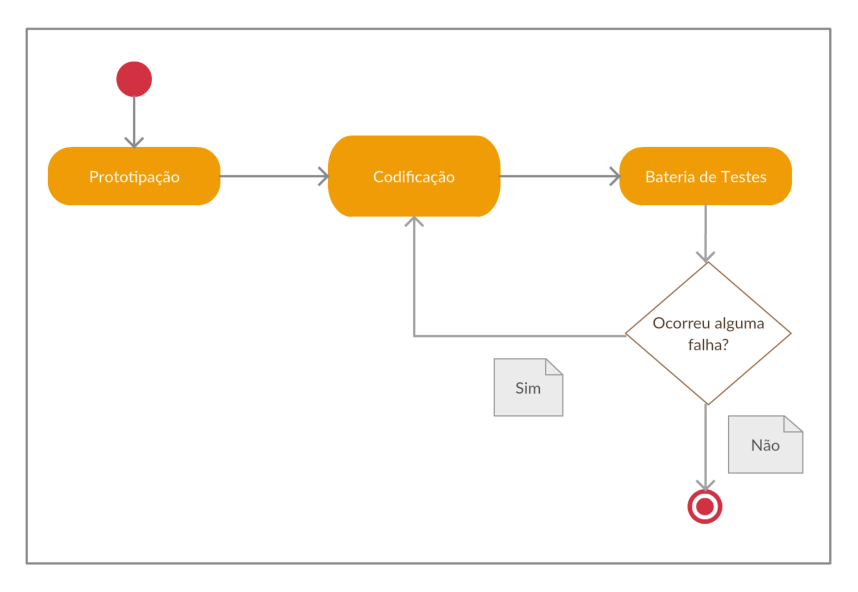
\includegraphics[width=.7\textwidth]{figuras/fluxograma_dev.eps} 
  \caption{Fluxograma de Desenvolvimento ``\acrshort{uft} Serviços''.}
  \label{fluxograma-dev} 
\end{figure} 

Conforme a Figura \ref{fluxograma-dev}, o modelo adotado para o desenvolvimento deste projeto propõe uma integração entre a metodologia de desenvolvimento ágil \textit{Scrum} e as boas práticas de desenvolvimento \textit{software}, utilizando-se de testes unitários e a criação de protótipos para validação de novas funcionalidades do sistema.

\section{Ambiente Computacional}

\noindent Nesta seção são demonstrados os ambientes computacionais utilizados para a construção (etapa de desenvolvimento) e funcionamento em produção do sistema ``\acrshort{uft} Serviços''. Desde a concepção deste projeto foi realizada uma pesquisa sobre quais tecnologias e conjunto de ferramentas de desenvolvimento de \textit{software} que possibilitaria a criação de um ambiente de programação flexível e que viabilizasse o gerenciamento de projetos de \textit{software} em equipe. Após a realização desta pesquisa foi escolhido o GIT\footnote{GIT: https://git-scm.com/} como ferramenta para o controle de versão do código fonte do projeto, tendo sua hospedagem feita em um conjunto de repositórios remotos de acesso privado no sistema Bitbucket\footnote{Bitbucket: https://bitbucket.org/}.

O motivo da escolha do GIT como sistema para o controle de versão se dá pelo fato dele ser uma das ferramentas mais consolidadas de versionamento de código fonte \cite{gitcontrole}. Sendo que, a motivação para a escolha do Bitbucket veio pela razão dele ser uma plataforma \textit{web} para hospedagem de projetos que utilizam o GIT, que tem como principal característica a criação ilimitada e gratuita de repositórios privados de código fonte \cite{bitbucket}.

Em conjunto com o GIT, foi adotado o conceito de integração contínua de desenvolvimento de \textit{software} através da ferramenta Jenkins\footnote{Jenkins: https://jenkins.io/}. O motivo para a escolha deste conceito se deu pelo fato da integração contínua ser uma prática que visa a integração frequente (várias vezes ao dia) de pequenas partes de código ao repositório principal de código-fonte, uma vez que, integrar pequenas partes facilita o tratamento dos possíveis problemas de integração, do que quando se integra partes maiores.

\subsection*{Ambiente de Desenvolvimento} 

\noindent O ambiente de desenvolvimento do ``\acrshort{uft} Serviços'' foi construído com base na arquitetura de desenvolvimento de aplicações corporativas \textit{Java Enterprise Edition} (Java EE)\footnote{Java EE: http://www.oracle.com/technetwork/java/javaee/overview/index.html}, padrão este que foi utilizado como suporte para a construção do sistema \textit{web} administrativo e aplicação de comunicação \acrshort{rest} API. 

Para o desenvolvimento do ambiente móvel foi utilizado o \gls{sdk}, disponibilizado pelo Google\footnote{Google: http://www.google.com} como padrão para construção de aplicações para o sistema operacional móvel Android\footnote{Android: https://www.android.com/}. Sendo que, uma característica presente em todas as aplicações descritas neste projeto está na utilização da linguagem de programação Java\footnote{Java: https://www.java.com}, como padrão de desenvolvimento de ambos os sistemas. 

A Figura \ref{ambiente_dev} demonstra o funcionamento do ambiente de desenvolvimento usado para a construção do sistema ``\acrshort{uft} Serviços''. O fluxo de programação inicia a partir do computador de desenvolvimento, onde estão instalados os ambientes de desenvolvimento integrado (IDE) Netbeans\footnote{Netbeans: https://netbeans.org/} e o Android Studio\footnote{Android Studio: https://developer.android.com/studio/index.html}, bem como o banco de dados necessário para que seja possível simular o ambiente de produção na máquina do programador. 

Na máquina do desenvolvedor está instalado o servidor \textit{web} \textit{Container} Java Jboss Wildfly\footnote{Wildfly: http://wildfly.org/}, servidor este que é responsável por receber todas as requisições \gls{http} do sistema \textit{web} administrativo, bem como todas as requisições feitas pelo aplicativo móvel Android presente nos \textit{smartphones} dos usuários. 

O GIT é utilizado para efetuar o controle de versão tanto do código fonte do aplicativo Android, como do sistema \textit{web}. Sendo que, todos esses repositórios estão também disponíveis remotamente no sistema Bitbucket, podendo estes serem acessados pelos programadores envolvidos no projeto que tenham suas respectivas permissões de acesso.

\begin{figure}[H]
  \centering
  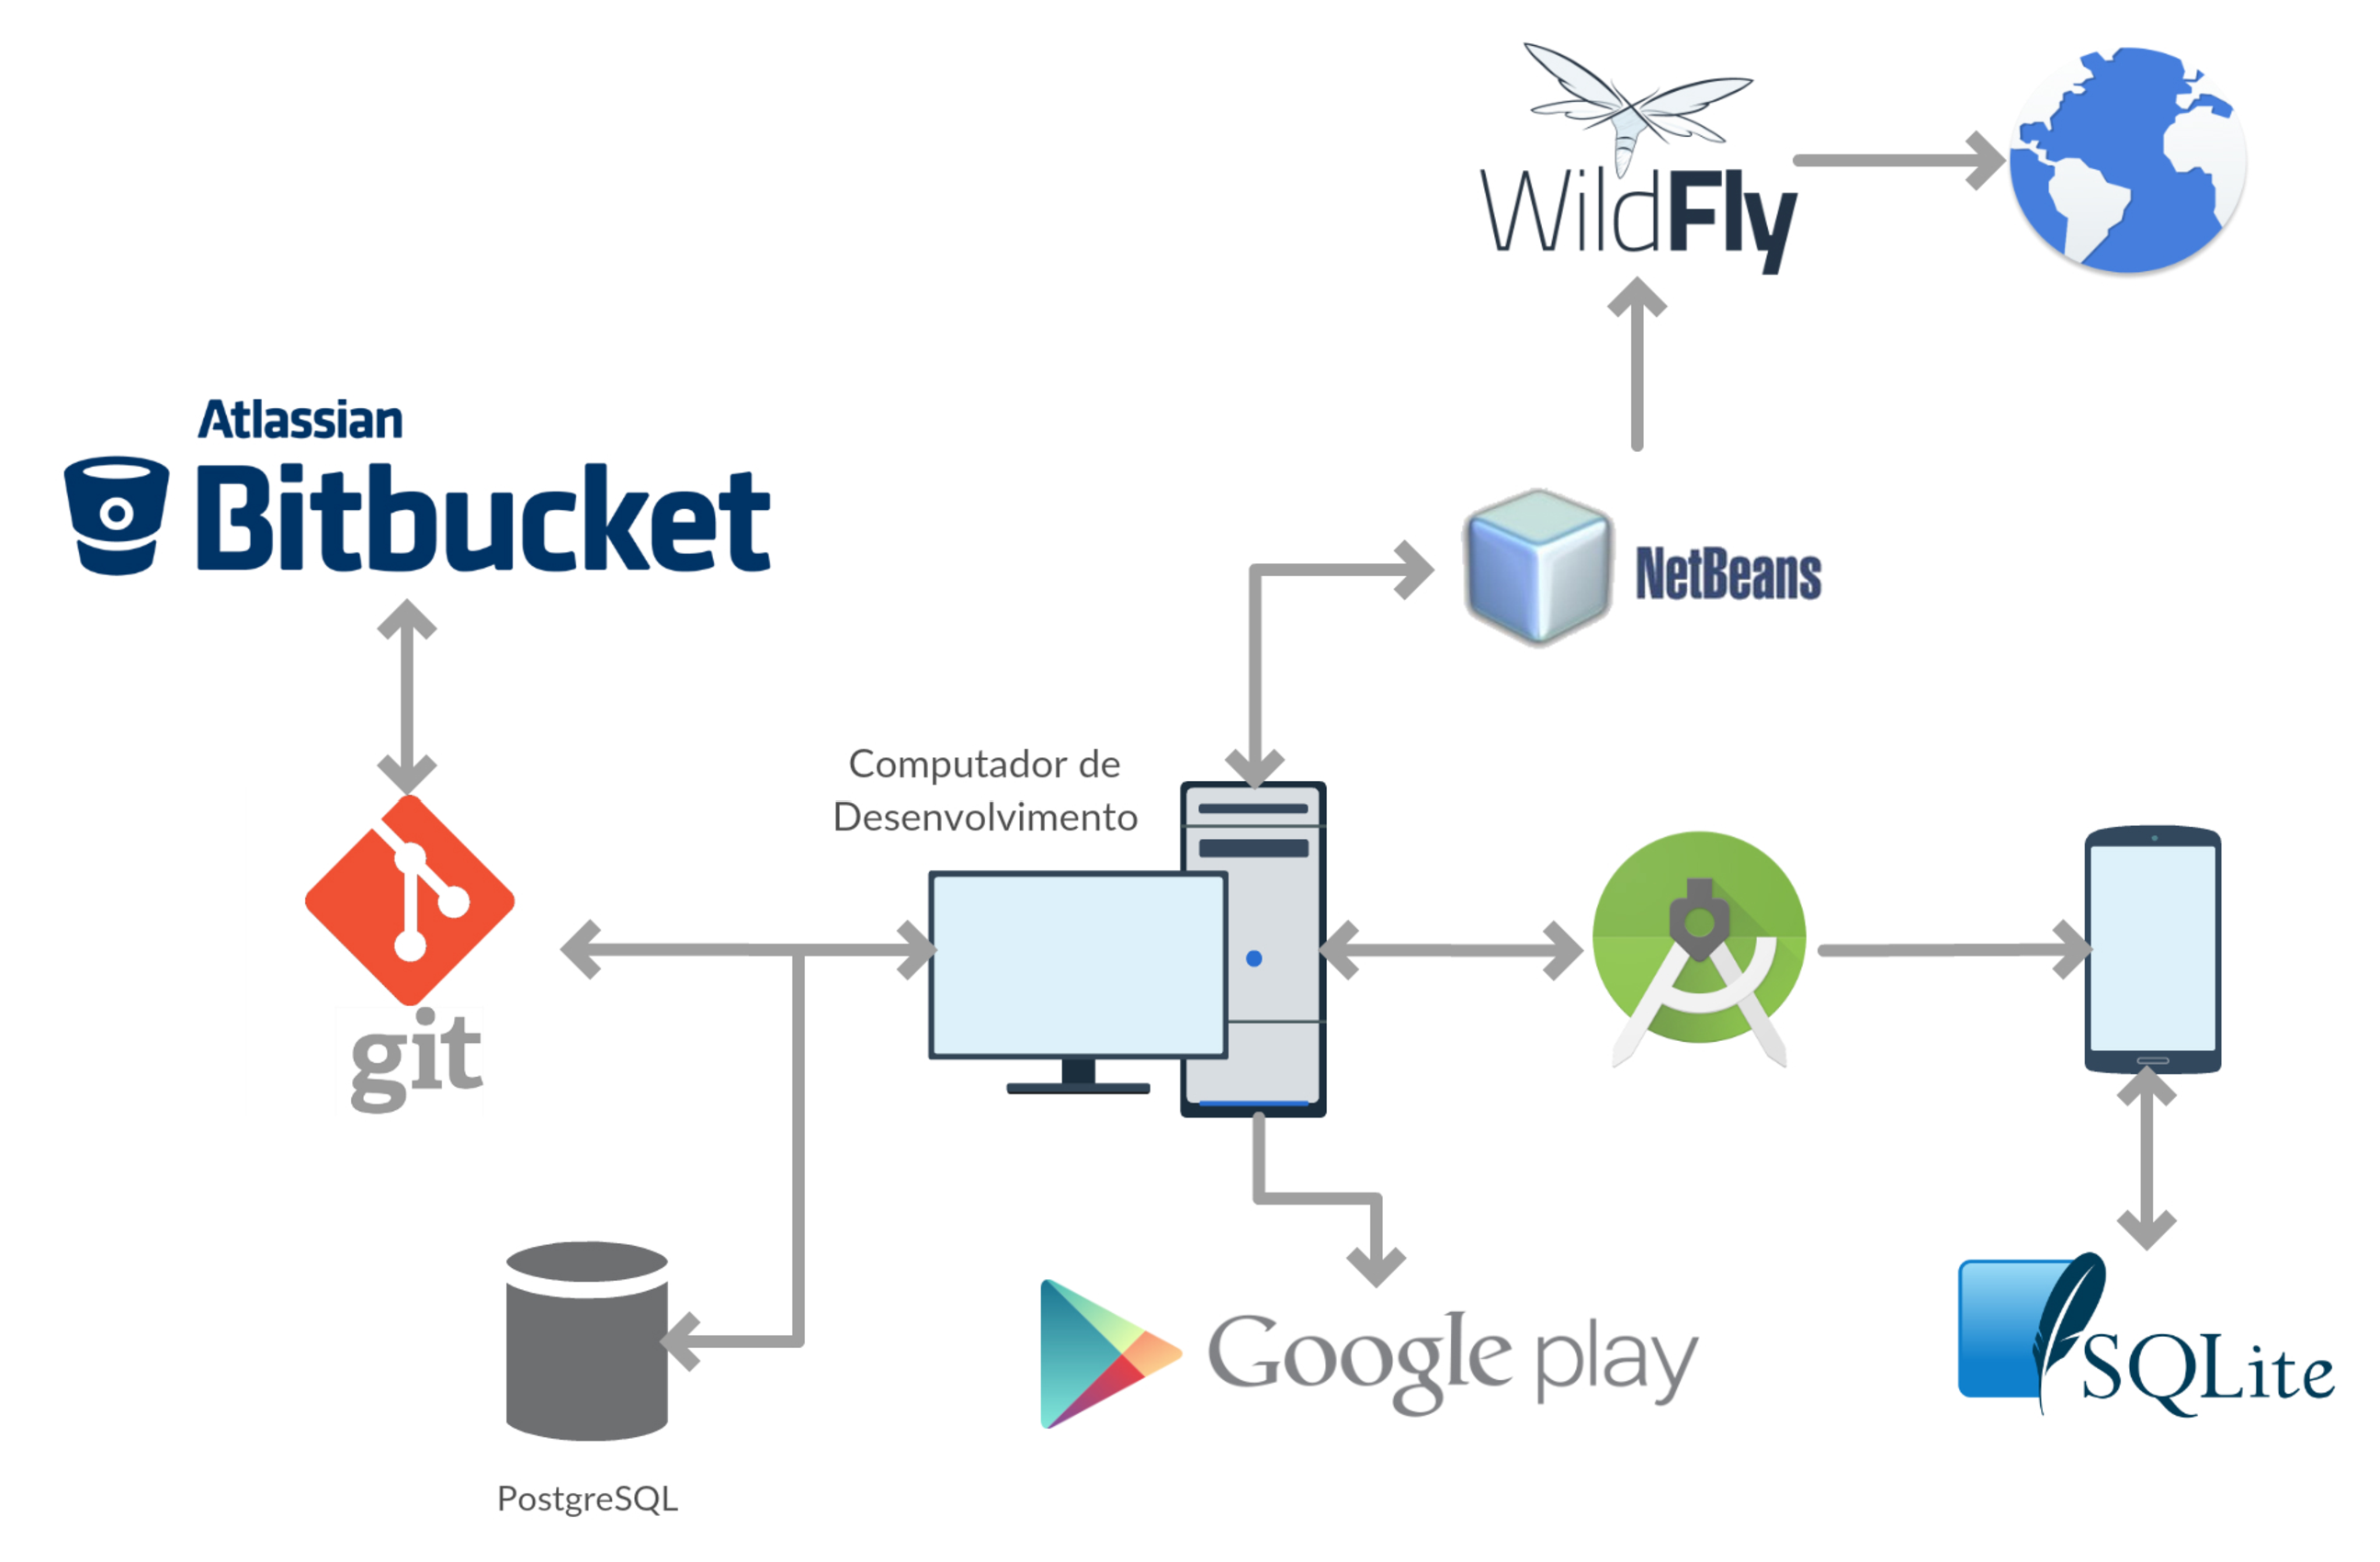
\includegraphics[width=0.7\textwidth]{figuras/develop.eps} 
  \caption{Ambiente de Desenvolvimento ``\acrshort{uft} Serviços''.}
  \label{ambiente_dev} 
\end{figure}

\subsection*{Ambiente de Produção}

\noindent O ambiente de produção foi montado de forma a automatizar as tarefas de atualização do Sistema \textit{web} administrativo do ``\acrshort{uft} Serviços''. O ambiente se concentra basicamente em três importantes servidores, sendo eles o Servidor de Banco de Dados, Servidor de Aplicação e Servidor de Integração Contínua.

A Figura \ref{ambiente_prod} demonstra o funcionamento do ambiente de produção, onde cada um dos servidores presentes desempenha um papel fundamental para o funcionamento do sistema. No servidor de banco de dados, onde está instalado o Banco de Dados Relacional PostgreSQL, há todas as informações dos chamados realizados pelo sistema móvel, e o histórico dos encaminhamentos realizados pelos usuários com acesso ao sistema \textit{web} administrativo. 

No Servidor de Aplicação (Wildfly), é onde fica hospedado a aplicação \textit{web} responsável por hospedar o sistema ``\acrshort{uft} Serviços'', além dele ser o responsável pela comunicação com o servidor de Banco de Dados do sistema e aplicativo móvel Android.

O Servidor de Integração Contínua é responsável por monitorar as modificações realizadas no repositório remoto no Bitbucket, onde a cada \textit{release}/\textit{commit} do \textit{software} ele é responsável por realizar o \textit{build} (etapa de compilação) e a execução de testes automatizados, através da definição de testes unitários definido pela a equipe de desenvolvedores. Sendo que, caso não ocorra nenhum erro durante este processo, é feito a atualização do sistema \textit{web} (deploy) no servidor de aplicação Wildfly.

\begin{figure}[H]
  \centering
  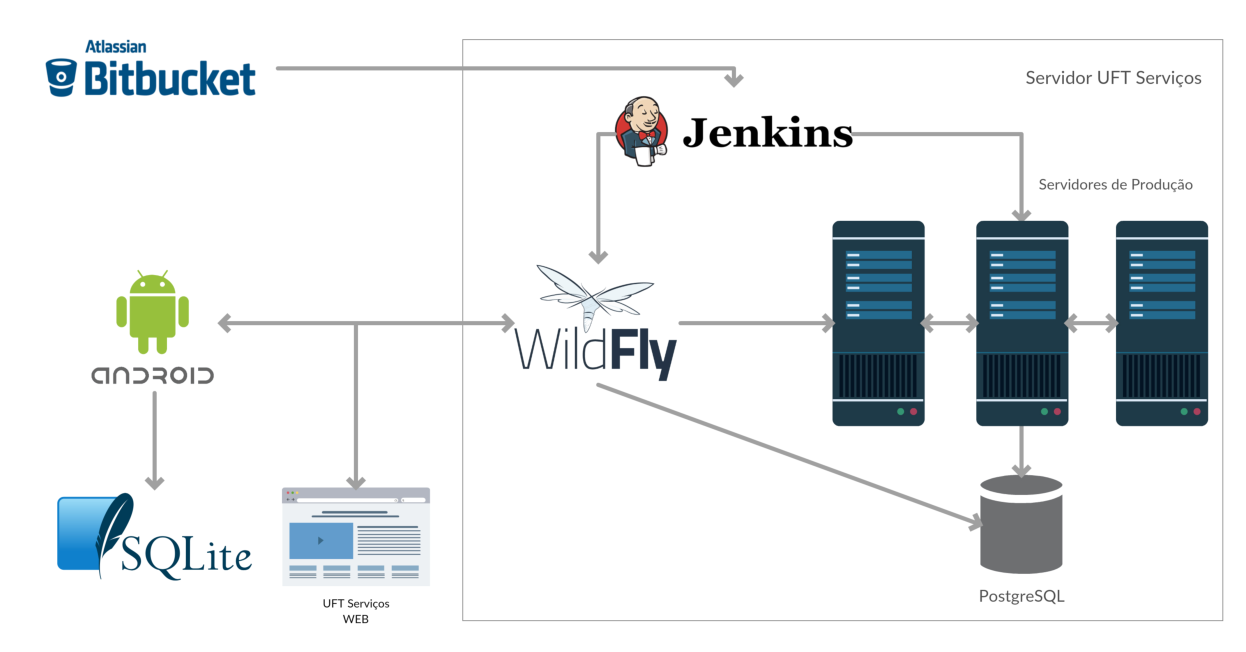
\includegraphics[width=0.7\textwidth]{figuras/production.eps} 
  \caption{Ambiente de Produção ``\acrshort{uft} Serviços''.}
  \label{ambiente_prod} 
\end{figure}

\section{Métodos}

\noindent Nesta seção é demonstrado os métodos aplicados para a construção e avaliação da etapa de desenvolvimento e implantação do sistema ``\acrshort{uft} Serviços''. Onde o objetivo deste capítulo é apresentar a aplicação dos métodos que foram retratados no Capítulo de Fundamentação Teórica, como a utilização do \acrshort{itil} v3, o modelo de desenvolvimento ágil \textit{Scrum} e a técnica utilizada para a avaliação da usabilidade do sistema, o \textit{System Usability Scale}.

\subsection*{Ciclo de Vida de Serviços (\acrshort{itil} v3)}

\noindent Dado as etapas do ciclo de vida de serviços do \acrshort{itil} v3 descrito na Fundamentação Teórica, foi realizada uma análise sobre quais de suas principais práticas seriam aplicadas neste projeto. A utilização das práticas do \acrshort{itil} v3 adotadas neste trabalho foi feita através da escolha de suas principais técnicas, sendo levado em consideração também o tempo para execução destas técnicas e que elas estejam dentro de um tempo hábil de implantação do sistema. 

A Figura \ref{itil_aply} demonstra todos os processos presentes na fundamentação do \acrshort{itil} v3, onde cada um dos processos apresentados compõem o ciclo de vida de serviços apresentado no Capítulo 2.

\begin{figure}[H]
  \centering
  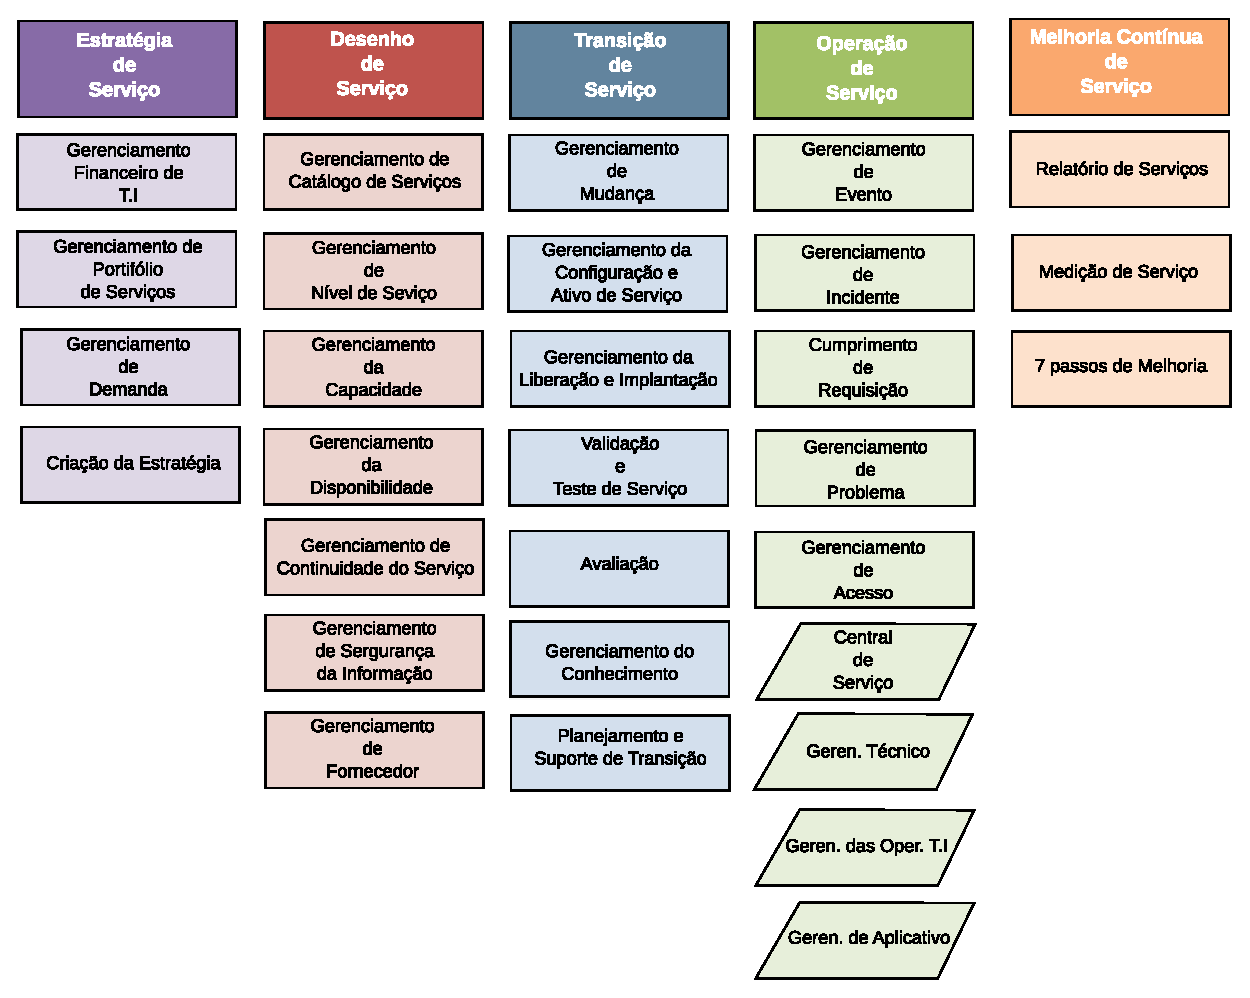
\includegraphics[width=0.7\textwidth]{figuras/itil_aply.eps} 
  \caption{Itens do Ciclo de Vida de Serviços \acrshort{itil} v3 (Adaptada de \cite{introductoryoverviewofitil}).}
  \label{itil_aply} 
\end{figure}

Após feita a análise sobre quais itens do \acrshort{itil} v3 seriam aplicados neste trabalho, foi decidido pela utilização das seguintes técnicas:

\begin{itemize}
    \item Estratégia de Serviços: através da Criação da Estratégia e Gerenciamento de Demanda;
    \item Desenho de Serviço: através do Gerenciamento de Nível de Serviço, Gerenciamento da Capacidade, Gerenciamento da Disponibilidade, Gerenciamento de Segurança da Informação e Gerenciamento de Fornecedor;
    \item Transição de Serviço: através do Gerenciamento de Mudança, Validação e Teste de Serviço, Avaliação e Gerenciamento do Conhecimento; e
    \item Melhoria Contínua de Serviço: através da Medição de Serviço.
\end{itemize}

\subsection*{Estratégia de Serviço}

\noindent Na etapa de Estratégia de Serviço foi utilizada o conceito de Gerenciamento de Demanda e Criação de Estratégia, que serviu como base para a criação da Estratégia de Serviço do sistema ``\acrshort{uft} Serviços''.

Em Gerenciamento de Demanda foi definido através da criação do Acordo de Nível de Serviço, onde foi definido como será realizado o gerenciamento da demanda do serviços presentes no acordo após a implantação do sistema ``\acrshort{uft} Serviços''.

Foi através da etapa de Criação de Estratégia que foi possível criar as perspectivas estratégicas de utilização do sistema ``\acrshort{uft} Serviços''. Sendo que a criação da estratégia de implantação deste projeto se baseou no modelo dos 4 Ps da estratégia, que é caracterizado por \cite{servicestrategy}:

\begin{itemize}
    \item Perspectiva: Onde é definido os valores da organização, através da definição da missão, visão e valores;
    \item Posição: Caracterizado pelo posicionamento da organização frente aos problemas enfrentados;
    \item Plano: Através da aplicação de um conjunto de estratégias para alcançar a visão e os objetivos da organização; e
    \item Padrão: Tem como característica a aplicação de processos e organizações para que os objetivos sejam satisfeitos.
\end{itemize}

\subsection*{Desenho de Serviço}

\noindent Durante a etapa de Desenho de Serviço, foi empregado os conceitos de Gerenciamento de Nível de Serviço, Gerenciamento de Capacidade, Gerenciamento de Disponibilidade, Gerenciamento de Segurança da Informação e Gerenciamento de Fornecedor. Cada um dos gerenciamentos mencionados foram aplicados durante a etapa de planejamento de desenvolvimento do sistema ``\acrshort{uft} Serviços''.

No Gerenciamento de Nível de Serviço, foi firmado um acordo entre os clientes do sistema e fornecedores, a partir da criação do \acrshort{ti} disponível no Apêndice IV. A partir da criação deste documento foram definidas informações como as responsabilidades que os prestadores de serviço de \acrshort{ti} tem com seus clientes e fornecedores, através da definição das responsabilidades em que todos os evolvidos tem com este acordo.

Na etapa de Gerenciamento de Capacidade, foram definidas informações que visam garantir que os serviços de \acrshort{ti} e infraestrutura tenham capacidade de atender os requisitos com relação a capacidade e que as informações presentes no gerenciamento de capacidade estejam de acordo com as necessidades dos utilizadores do sistema.

Como parte do Gerenciamento de Disponibilidade do sistema, foi criado em forma de documento o Plano de Gestão de Disponibilidade do sistema ``\acrshort{uft} Serviços'' neste documento estão presentes informações que contém um conjunto de direcionamentos que visam manter o alinhamento das estratégias de negócio da organização que foram definidas na \acrshort{ti}.

Na fase de Gerenciamento de Segurança da Informação, foram definidas as medidas de segurança de forma que haja um alinhamento com as necessidades da organização e com os requisitos de privacidade dos dados armazenados dos usuários. Por conta de se tratar de modelo incremental de segurança, foram definidos inicialmente os requisitos de autenticação do sistema e que os dados referentes a abertura de um chamado sejam apenas compartilhados, entre o solicitante e o administrador do sistema.

A etapa de Gerenciamento de Fornecedor foi utilizada para garantir que os fornecedores externos ao serviço oferecido pelo sistema estejam de acordo com as metas e expectativas de negócio da organização e de seus clientes. Foi através da definição do gerenciamento de fornecedores que foi possível gerenciar o desempenho dos fornecedores e negociação de contratos durante o ciclo de vida do acordo.

\subsection*{Transição de Serviço}

\noindent Na etapa de Transição de Serviço foi utilizado os conceitos de Gerenciamento de Mudanças, Validação e Teste de Serviço, Avaliação e Gerenciamento do Comportamento. Sendo que cada uma das etapas foram aplicadas durante a fase de transição de serviço do sistema.

A fase de Gerenciamento de Mudanças foi aplicada para minimizar o impacto causado pela necessidade da aplicação de mudanças críticas no sistema e seu principal objetivo é otimizar a exposição a riscos e prevenir o surgimento de transtornos aos utilizadores do \textit{software}.

A utilização de Validação e Testes de Serviço foi de grande importância para o planejamento da aplicação de novas funcionalidades e correções dos erros encontrados no sistema. Foi através desta etapa em conjunto com práticas de programação orientada a testes e integração contínua do \textit{software}, que foi possível fazer uma validação mais segura referente a atualização do sistema em produção de forma automatizada.

Na fase de Avaliação, utilizou-se os \textit{feedbacks} das  a apresentação das novas funcionalidades do sistema aos envolvidos no projeto e as sugestões de mudanças propostas pelos clientes do sistema. A etapa de avaliação foi de grande importância, pois ela forneceu um conjunto de informações com relação à experiência do usuário que influenciaram na criação de adaptações das funcionalidades do sistema.

A etapa de Gerenciamento do Conhecimento foi aplicada para a melhoria da gestão de tomada de decisão, assegurando que informações precisas estejam disponível de forma clara em todo o ciclo de vida de serviços. A utilização da gestão de conhecimento foi de grande importância durante a implantação do sistema ``\acrshort{uft} Serviços'', pois a partir da gestão efetiva do conhecimento foi possível criar uma documentação clara contendo as informações referentes ao desenvolvimento e implantação do sistema.

\subsection*{Melhoria Contínua de Serviço}

\noindent A etapa de Melhoria Contínua do Serviço foi uma das etapas mais importantes da aplicação das práticas do \acrshort{itil} v3 neste projeto, foi a partir dela que foi possível mensurar os serviços oferecidos pelo sistema através da etapa de Medição do Serviço.

Na etapa de Medição do Serviço, foi possível mensurar através de ferramentas de monitoramento, o comportamento do sistema e de seus usuários, através do monitoramento da infraestrutura de \textit{hardware} que mantém o sistema no ar e das informações básicas sobre o usuário, como a idade, o sexo e o histórico de navegação durante a utilização do aplicativo móvel.

Uma outra forma de medição do serviço oferecido pelo sistema foi a partir da aplicação do teste de usabilidade  \acrshort{sus}, sua aplicação em conjunto com as outras informações geradas pela medição do serviço foi de grande importância, pois possibilitou uma avaliação efetiva sobre os ganhos obtido pela implantação do sistema.

\subsection*{Desenvolvimento Ágil (\textit{Scrum})}

\noindent A utilização \textit{Scrum} foi crucial para a organização das atividades necessárias para a conclusão do desenvolvimento do sistema, em conjunto com as práticas de desenvolvimento ágil \textit{Scrum} foi utilizado o modelo de organização de tarefas chamado \textit{Kanban} \cite{anderson2010kanban}. A Figura \ref{quadro-kanban} demonstra como é o funcionamento dessa técnica, onde basicamente as tarefas são divididas em três ou mais colunas contendo uma identificação única para um dado conjunto de tarefas, representada através de anotações em \textit{post-it}.

Neste projeto foi utilizado três colunas para representar as atividades realizadas, sendo elas tarefas: Á fazer, Em desenvolvimento e Finalizado. Na coluna de tarefas Á fazer é onde é colocada todas as novas tarefas a serem realizadas. Nas tarefas Em desenvolvimento é colocada todas as tarefas que foram iniciadas, mas ainda não foram concluídas. Na coluna Finalizado é colocada todas as tarefas que foram finalizadas. Para um melhor acompanhamento das demandas do sistema ``\acrshort{uft} Serviços'', foi utilizado a ferramenta colaborativa de organização de tarefas chamada Trello\footnote{Trello: https://trello.com/}.

\begin{figure}[H]
 \centering
 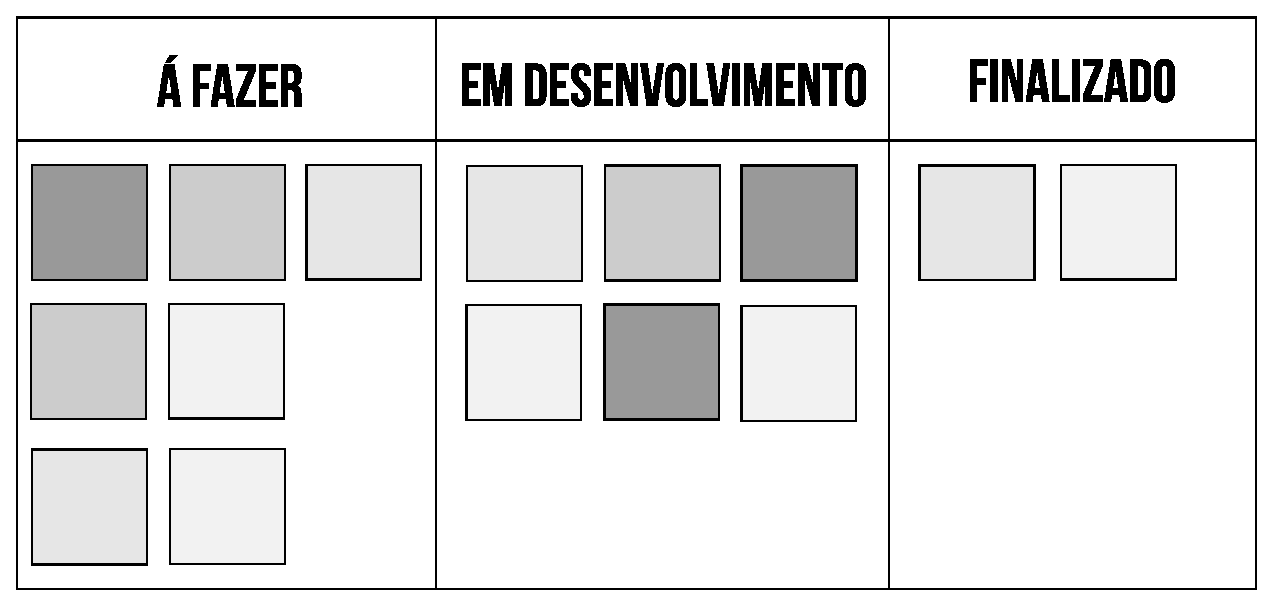
\includegraphics[width=0.7\textwidth]{figuras/kanban.eps} 
 \caption{Quadro de atividades Kanban.}
 \label{quadro-kanban} 
\end{figure}

Todas as atividades realizadas neste projeto foram baseadas na metodologia de desenvolvimento ágil \textit{Scrum}, através do conceito de organizações dos \textit{backlog} e das demandas a serem entregas a partir da definição dos \textit{sprints}, sendo que o acompanhamento do projeto foi feito a partir de reuniões periódicas em conjunto com os demais envolvidos no projeto.

\subsection*{Teste de Usabilidade (\textit{System Usability Scale})}

\noindent A realização do teste de usabilidade é um dos pontos fundamentais para avaliação do resultado do \textit{software} desenvolvido neste trabalho. Através da realização deste teste é possível identificar os principais pontos positivos e negativos com relação a usabilidade do sistema ``\acrshort{uft} Serviços'', podendo ser averiguado itens como a facilidade do uso do sistema, a eficiência e se o usuário se sente confortável em estar utilizando o sistema pela primeira vez.

O teste utilizado neste projeto é o \textit{System Usability Scale} (SUS) que consiste em um questionamento contendo 10 afirmativas que abrangem as seguintes possibilidade de respostas: Discordo Totalmente, Discordo, Neutro, Concordo e Concordo Totalmente. Uma característica importante do  \acrshort{sus} é que nele somente é permitido aos usuários uma única resposta por pergunta e que sua aplicação sempre ocorre logo após a utilização do sistema pelo usuário. O \acrshort{sus} se caracteriza como um modelo para averiguação da usabilidade que procura mensurar o nível de facilidade de uso de um sistema, tendo como foco em três pontos fundamentais que é a efetividade, eficiência e a satisfações dos usuários do sistema \cite{bangor2009determining}. No Apêndice II é apresentado o formulário utilizado para realização do teste de usabilidade.

Cada resposta feita no questionário do \acrshort{sus} tem uma escala de variação que vai de 1 a 5, onde 1 significa que o usuário discorda totalmente e 5 que ele concorda plenamente com o que está sendo questionado \cite{bangor2009determining}. 

Para saber se um sistema é de boa usabilidade ou não o \acrshort{sus} aplica o seguinte conjunto de regras: primeiramente é subtraído por 1 todas as respostas de questões de numeração ímpar (1, 3, 5, 7, 9) e subtraído por 5 todas as questões pares (2, 4, 6, 8, 10). Após fazer a devida subtração de cada item deve-se fazer um somatório dos valores obtidos de cada questão e multiplicar por 2.5, assim obtendo uma pontuação resultante variando do intervalo de 0 a 100. Para que um sistema seja caracterizado minimamente usável deve-se obter a pontuação mínima de 68 pontos, sendo que notas menores a 68 caracteriza o sistema avaliado como de baixa usabilidade \cite{Brooke:2013:SR:2817912.2817913}.

A Figura \ref{escala-sus} mostra a distribuição dos níveis de usabilidade do  \acrshort{sus}, como pode ser observado o  \acrshort{sus} possui uma escala que compreende os níveis F, D, C, B e A. Cada um dos níveis apresentados representa um intervalo de nota referente a nota obtida pela avaliação do  \acrshort{sus}, sendo a pior nota representada pela letra F e a melhor pela letra A.

\begin{figure}[H]
 \centering
 \includegraphics[width=1\textwidth]{figuras/escala_sus.png} 
 \caption{Distribuição dos níveis de usabilidade do \textit{System Usability Scale} (SUS) (Adaptado de \cite{bangor2009determining}).}
 \label{escala-sus} 
\end{figure}

Na Tabela \ref{tabela-sus} mostra a distribuição dos intervalos de notas do  \acrshort{sus} e suas respectivas classificações. Como pode ser observado, a classificação do  \acrshort{sus} pode variar entre cinco principais resultados, sendo eles: Ruim, Razoável, Bom, Excelente e Muito Excelente.

\begin{table}[H]
    \centering
    \small
    \begin{tabular}{|c|c|c|}
    \hline
    \multicolumn{1}{|l|}{Atribuição} & \multicolumn{1}{l|}{Classificação} & \multicolumn{1}{l|}{Variação de Nota} \\ \hline
    F                                & Ruim                               & x $\leq $ 60                        \\ \hline
    D                                & Razoável                           & 60  \textless x $\leq$ 70          \\ \hline
    C                                & Bom                                & 60 \textless x $\leq$ 80           \\ \hline
    B                                & Excelente                          & 80 \textless x $\leq$ 90           \\ \hline
    A                                & Muito Excelente                    & x $\geq$ 90                     \\ \hline
    \end{tabular}
    \caption{Tabela de classificação do \textit{System Usability Scale} (SUS).}
    \label{tabela-sus}
\end{table}

Como pode ser observado, o \acrshort{sus} classifica o sistema através da nota média obtida pela aplicação da fórmula descrita anteriormente no início desta seção. Sendo que, para valores menores que 60 o sistema é classificado como um \textit{software} de baixa usabilidade, se a nota for entre 60 e 70 ele é classificado como de usabilidade razoável, nota entre 60 e 80 o sistema é classificado como de boa usabilidade, se o resultado for entre 80 e 90 o sistema é classificado como de excelente usabilidade e por fim se a nota for maior que 90 o sistema é classificado como Muito Excelente no quesito usabilidade.

\section{Diagramas \acrshort{uml}}

\noindent Nesta seção são apresentados os diagramas \textit{Unified Modeling Language} (UML) utilizadas para criação do sistema ``\acrshort{uft} Serviços'', onde foi decidido devido a necessidade de que ocorra o desenvolvimento do sistema que esteja de acordo com o que foi planejado inicialmente no levantamento de requisito pela criação do Diagrama de Caso de Uso da utilização do sistema, o Diagrama de Classe (Sistema \textit{web} e \textit{Mobile}), o Diagrama de Atividade contendo as principais atividades da utilização do sistema e o Diagrama de Implantação.

\subsection*{Diagrama de Caso de Uso}

Para exemplificar melhor o \textit{workflow} de funcionamento do sistema ``\acrshort{uft} Serviços'' foi criado um diagrama geral de caso de uso, conforme apresentado na Figura \ref{diagram-uml-casodeuso}. Neste diagrama é demonstrado uma visão geral sobre os principais atores presentes na utilização do sistema, sendo eles o corpo docente, discente, técnico administrativo e a central de atendimento dos chamados.

\begin{figure}[H]
 \centering
 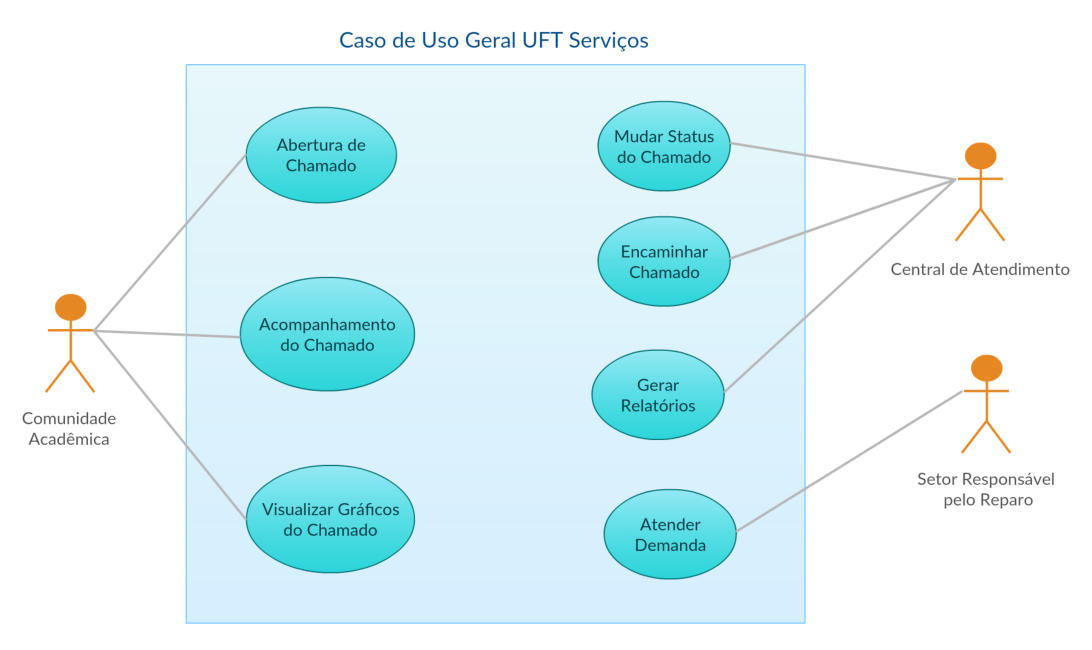
\includegraphics[width=1\textwidth]{figuras/uml-casodeuso.eps} 
 \caption{Diagrama de Caso de Uso Geral sistema ``\acrshort{uft} Serviços''.}
 \label{diagram-uml-casodeuso} 
\end{figure}

O diagrama demonstra todas as atividades que podem ser exercidas por cada um dos atores mencionados, como pode ser observado a comunidade acadêmica pode utilizar o sistema realizando chamados, acompanhando e fiscalizando a solução dos problemas além de poder visualizar os gráficos do chamado. Já na parte administrativa do sistema fica a cargo da Central de Atendimento realizar a mudança do estágio do chamado o seu encaminhamento e a geração dos relatórios, e por fim o ator intitulado Responsável pelo Reparo é responsável por estar executando a ordem de serviço.

\subsection*{Diagrama de Classe}

\noindent Nesta seção é apresentados os diagramas de classe do Sistema \textit{web} e do Sistema \textit{Mobile}, onde a partir da definição destes diagramas foram criadas as classes e a lógica de negócio da aplicação. Durante o desenvolvimento desta modelagem foi feito da forma mais enxuta possível, de forma que ao criar as classes do sistema não houvesse nenhuma dificuldade durante sua implementação, fornecendo um baixo acoplamento de código.

Como pode ser observado a seguir é mostrado os diagramas de classe que foram criados onde são demonstradas todas as principais classes de domínio que compõem o sistema ``\acrshort{uft} Serviços'', apresentando informações como os atributos e métodos pertencentes a cada uma das classes existentes em ambos os sistemas. A seguir as Figuras \ref{diagram-android} e \ref{diagram-web} é demonstrado os diagramas de classe do sistema.

O primeiro diagrama de atividade apresentado pela Figura \ref{diagram-android} é exemplificado o processo de abertura de um chamado pelos usuários do sistema através do aplicativo Android. O processo consiste na seleção de uma categoria de chamado cadastrado no sistema e a validação do formulário a partir do preenchimento de informações como o título, descrição, localização e foto do chamado. Após a validação do formulário de abertura do chamado as informações são então serializadas e enviadas pela rede para o servidor de aplicação do ``\acrshort{uft} Serviços''.

O diagrama apresentado na Figura \ref{diagram-web} apresenta o processo de cadastro e autenticação do usuário no aplicativo móvel, o processo consiste no preenchimento e validação do formulário de cadastro de usuário. Após a validação é enviado as informações para o servidor de aplicação é criado um usuário com o \textit{status} inativo e enviado um \textit{e-mail} de ativação do usuário, logo em seguida caso o usuário clique no \textit{link} de ativação o seu \textit{status} será mudado para ativo e com isso o usuário poderá logar no sistema a partir do aplicativo Android.

\begin{figure}[H]
 \centering
 \includegraphics[angle=270, width=1\textwidth]{figuras/uft-servicos-android-diagram} 
 \caption{Diagrama de classes do sistema ``\acrshort{uft} Serviços'' Android.}
 \label{diagram-android} 
\end{figure}

\begin{figure}[H]
 \centering
 \includegraphics[angle=270, width=0.9\textwidth]{figuras/uft-servicos-diagram} 
 \caption{Diagrama de classes do sistema ``\acrshort{uft} Serviços'' web administrativo.}
 \label{diagram-web} 
\end{figure}

\subsection*{Diagrama de Atividade}

\noindent Para um melhor entendimento sobre o processo de criação de usuário e abertura de chamado realizado pelo ``\acrshort{uft} Serviços'', foi criado dois digramas de atividade que demonstram as atividades que podem ser realizados pelo usuário durante a utilização do sistema. Nos diagramas a seguir é exposto todo o procedimento realizado para o cadastro do usuário no sistema e o procedimento realizado para a abertura de um chamado. A seguir na Figura \ref{diagram-atividade} é apresentado os diagramas de atividades mencionados.

O primeiro diagrama de atividade apresentado na Figura \ref{diagram-atividade} exemplifica o processo de abertura de um chamado pelos usuários do sistema através do aplicativo móvel. O processo consiste na seleção de uma categoria de chamado e a validação do formulário através do preenchimento de informações como o título, descrição, localização e foto do chamado. Sendo que após a validação do formulário de abertura do chamado as informações são enviadas para o servidor de aplicação do sistema ``\acrshort{uft} Serviços''.

O diagrama apresentado na Figura \ref{diagram-web} apresenta o processo de cadastro e autenticação do usuário no aplicativo móvel, onde o processo consiste no preenchimento e validação do formulário de cadastro de usuário. Após a validação do formulário é enviado as informações para o servidor de aplicação e criado um novo usuário com o \textit{status} inativo. O sistema então envia um \textit{e-mail} de ativação do usuário, onde caso o usuário clique no \textit{link} de ativação o seu \textit{status} será mudado para ativo e consequentemente o usuário poderá realizar a autenticação no sistema.

\begin{figure}[H]
 \centering
 \includegraphics[width=1\textwidth]{figuras/atividade} 
 \caption{Diagramas de Atividade criação de usuário e autenticação e Processo de Abertura de Chamado.}
 \label{diagram-atividade} 
\end{figure}

\subsection*{Diagramas de Implantação}

\noindent O Diagramas de Implantação apresenta informações através da definição de nós, onde cada nó representa um módulo do sistema desenvolvido além de demonstrar os padrões e protocolos de comunicação em que cada nó faz com os demais. Como pode ser observado na Figura \ref{deployment_diagram} é apresentado modelo de diagrama de implantação adotado para a concepção do sistema ``\acrshort{uft} Serviços''.

\begin{figure}[H]
 \centering
 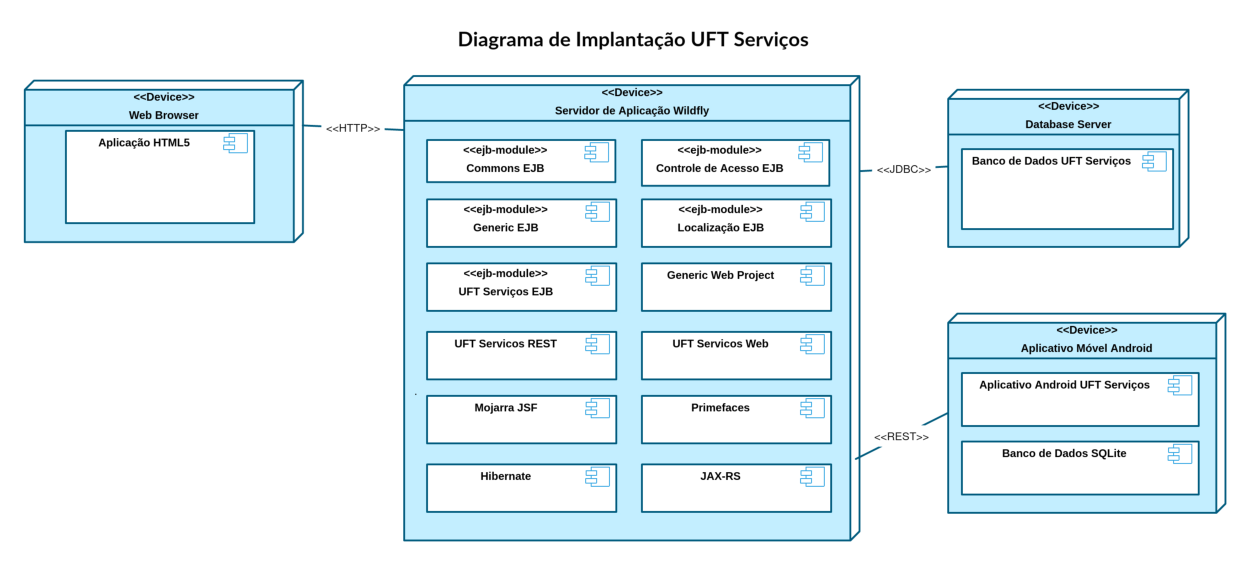
\includegraphics[width=1\textwidth]{figuras/deployment_diagram} 
 \caption{Diagramas de Implantação sistema ``\acrshort{uft} Serviços''.}
 \label{deployment_diagram} 
\end{figure}

Uma característica do sistema desenvolvido é o fato que a aplicação foi organizada em módulos \gls{ejb}, onde cada módulo \acrshort{ios} apresentado é responsável por uma tarefa específica no sistema. Outro ponto importante é os protocolos e padrões de comunicação adotado para comunicação do sistema, dentre eles está o protocolo \acrshort{http} e padrões de comunicação \acrshort{rest} e \gls{jdbc}.

\section{Ferramentas e Materiais}

\noindent Nesta seção é descrita as ferramentas utilizadas para o desenvolvimento do sistema ``\acrshort{uft} Serviços'', onde é descrito a funcionalidade de cada uma das ferramentas, as versões utilizadas no sistema e o motivo de sua utilização. Abaixo é listado todas as principais ferramentas que compõem o sistema ``\acrshort{uft} Serviços''.

\begin{enumerate}

    \item O \gls{javaee}\footnote{JavaEE: http://www.oracle.com/technetwork/java/javaee/overview/index.html} é um padrão de desenvolvimento de software corporativo oferecido pela Oracle para a comunidade de programadores Java. O Java EE é desenvolvido usando a \textit{Java Community Process} (JCP), através de contribuições de especialistas da indústria, organizações comerciais e comunidade de desenvolvedores de código \textit{open-source}.
    
    \item O \gls{jsf}\footnote{\acrshort{jsf}: https://javaserverfaces.java.net/} é um conjunto de especificações baseado no padrão MVC para construção de aplicações e interfaces \textit{web} com o usuário do lado cliente-servidor. O \acrshort{jsf} é baseado na abordagem de desenvolvimento orientado a componentes (\textit{component-based}) para construção de interfaces gráficas para a \textit{web}. O desenvolvimento de aplicações \acrshort{jsf} tem como base a orientação a eventos, característica essa que tem como propósito tornar mais prático o desenvolvimento de aplicações \textit{web} com o foco em oferecer aos desenvolvedores um ambiente de programação focado no desenvolvimento das regras de negócio da aplicação. A implementação padrão \acrshort{jsf} utilizada é o Mojarra 2.2.
    
    \item O Primefaces\footnote{Primefaces: http://www.primefaces.org/} é uma biblioteca \textit{open-source} de componentes que tem como propósito fornecer uma extensão aos componentes padrões presentes no \textit{Java Server Faces}.  Sua escolha foi feita devido a sua facilidade de utilização além da vasta opção de componentes presentes na biblioteca. A versão utilizada neste trabalho é a \textit{Primefaces Community} 5.3.
    
    \item O Materialize\footnote{Materialize: http://materializecss.com/} é uma biblioteca  \acrshort{css} para a criação de interfaces gráficas para \textit{web} utilizando o padrão de design Material Design\footnote{Material Desing: https://material.google.com/}. O motivo da escolha do Materialize foi por conta da facilidade de criação de layouts em HTML5 baseado no padrão Material Design.
    
    \item O Simple Grid é uma ferramenta em  \acrshort{css} para criação de \textit{grids} para organização de \textit{layout} da aplicação \textit{web} do ``\acrshort{uft} Serviços''. Sua escolha foi feita devido sua simplicidade para a criação de \textit{grid} e também por seu tamanho ser pequeno em relação a outras bibliotecas  \acrshort{css} com a mesma finalidade.
    
    \item O \gls{jpa}\footnote{JPA: http://www.oracle.com/technetwork/java/javaee/tech/persistence-jsp-140049.html} é uma especificação que fornece aos desenvolvedores um ambiente de desenvolvimento \gls{poo} baseado no \gls{pojo}. O modelo \acrshort{pojo} tem como objetivo tornar simplificado a forma como os desenvolvedores lidam com a persistência de dados através de abstrações do modelo banco de dados relacional para o ambiente de desenvolvimento orientado a objeto. A versão do \acrshort{jpa} utilizada no projeto é a implementação desenvolvida pela Red Hat\footnote{Red Hat: https://www.redhat.com/}, o Hibernate\footnote{Hibernate: http://hibernate.org/} 5.
    
    \item O sistema de banco de dados relacional utilizado neste trabalho é o o PostgreSQL\footnote{PostgreSQL: http://www.postgresql.org/}. Sua escolha foi feita devido sua estabilidade e sua capacidade de manter a integridade dos dados. Outra motivação para escolha do PostgreSQL é sua ampla documentação e comunidade de usuários ativa, além do fato dele ser o banco de dados \textit{open-source} mais utilizado no mundo. A versão do PostgreSQL utilizada neste projeto é a 9.5.
    
    \item O Apache Maven\footnote{Apache Maven: https://maven.apache.org/} é uma ferramenta para gerenciamento de dependências Java de uso fundamental para construções do sistema \textit{web} do ``\acrshort{uft} Serviços''. Suas funcionalidades vão além de um gerenciamento de dependências, mas também como uma ferramenta para automatização de compilação (build) de projetos construídos em Java. A versão do Apache Maven utilizado no projeto é a 3.3.9.
    
    \item O Apache Shiro\footnote{Apache Shiro: http://shiro.apache.org/} é um \textit{framework} de controle de acesso utilizado no sistema \textit{web} do ``\acrshort{uft} Serviços''. A versão utilizada neste trabalho é a 1.2.4.
    
    \item O Pretty Faces\footnote{Pretty Faces: http://www.ocpsoft.org/prettyfaces/} é uma ferramenta para criação de URL's amigáveis através da definição de contextos específicos para cada uma das páginas do sistema. A versão utilizada neste trabalho é a 2.0.12.
    
    \item O JAX-RS\footnote{JAX-RS: https://jax-rs-spec.java.net/} é uma API e especificação para construção de serviços \textit{web} de comunicação REST-API para a plataforma Java. A versão utilizada neste trabalho é a 2.0.
    
    \item O servidor \textit{web container} utilizado neste trabalho é o Wildfly\footnote{Wildfly: http://wildfly.org/}. Sua utilização se dá pelo fato de sua ampla comunidade de usuários e números de \textit{releases} e correções feitas periodicamente. A versão do Wildfly utilizado neste trabalho é a 10.
    
    \item O servidor para integração contínua utilizado para realização dos \textit{builds} e testes automatizados do sistema ``\acrshort{uft} Serviços'' é o Jenkins\footnote{Jenkins: https://jenkins.io/}, sua utilização foi feita devido ser o sistema de integração contínua de \textit{software} de código aberto mais popular no mercado, além de suas diversas possibilidades de configuração e sistema de \textit{plugins}. A versão do Jenkins utilizada neste projeto é a 2.0.
    
    \item O Android \acrshort{sdk}\footnote{Android \acrshort{sdk}: http://developer.android.com/intl/pt-br/sdk/index.html} é a biblioteca padrão utilizada para desenvolvimento de aplicativos para a plataforma Android OS.
    
    \item A IDE utilizada para desenvolvimento da aplicação móvel é o Android Studio\footnote{Android Studio: http://developer.android.com/intl/pt-br/sdk/index.html}. Sua utilização se dá pelo fato de seu amplo suporte e por ser a \acrshort{ide} oficial para desenvolvimento de aplicativos móveis para plataforma Android. A versão utilizada para desenvolvimento do aplicativo móvel ``\acrshort{uft} Serviços'' é a 2.1.
    
    \item A \acrshort{ide} utilizada para desenvolvimento do sistema \textit{web} e REST do ``\acrshort{uft} Serviços'' é o Netbeans\footnote{Netbeans: https://netbeans.org/}. Sua escolha foi feita devido seu amplo suporte à criação de aplicações Java e sua estabilidade e funcionalidades oferecidas pela \acrshort{ide}. A versão do Netbeans utilizada neste trabalho é a 8.1.
    
    \item O Ubuntu OS\footnote{Ubuntu: http://www.ubuntu.com/} é um sistema operacional \textit{open-source} baseado no \textit{kernel} Linux mais utilizado no mundo. Sua utilização é feita tanto no ambiente de desenvolvimento como no ambiente de produção, a versão utilizada no projeto é o Ubuntu 14.04.4 LTS.
    
    \item O Netdata\footnote{Netadata: https://github.com/firehol/netdata} é um sistema de monitoramento \textit{open-source} de \textit{hardware} e rede. Sua escolha foi feita devido sua facilidade de configuração e o número de gráficos que é apresentado pelo sistema.
    
    \item O Google \textit{Analytics}\footnote{Google Analytics: https://analytics.google.com/} é um sistema \textit{web} para monitoramento de acesso dos usuários do aplicativo móvel do ``\acrshort{uft} Serviços''. Sua utilização foi feita devido a facilidade de configuração da API de monitoramento no aplicativo Android e por fornecer diversas informações sobre o usuário como sexo, idade e região. Outra motivação para escolha da ferramenta é por conta do Google \textit{Analytics} oferecer em detalhes informações como o rastreamento de exceções, quais telas o usuário acessou durante o uso do aplicativo e a quantidade usuários que estão utilizando o sistema no momento.

\end{enumerate}

\section*{Considerações finais sobre o capítulo}

\noindent Neste capítulo foi apresentado os principais conceitos utilizados para a construção do sistema ``\acrshort{uft} Serviços'', sendo apresentado o ambiente computacional, os métodos, os diagramas \acrshort{uml} e as ferramentas utilizadas no sistema.

A utilização do \acrshort{itil} v3, \textit{Scrum} e aplicação do teste de usabilidade  \acrshort{sus} foram de grande importância para o desenvolvimento e implantação do \textit{software}. Através da aplicação dos conceitos apresentados foi possível obter uma base sólida quando a organização dos processos e serviços utilizados para implantação e manutenção do ``\acrshort{uft} Serviços''.

% ----------------------------------------------------------------------------------------------------- %
% Desenvolvimento
% ----------------------------------------------------------------------------------------------------- %

%\chapter{Desenvolvimento}

\noindent Este capítulo apresenta detalhadamente o processo de desenvolvimento das aplicações do ``UFT Serviços'' (Web, REST API e \textit{Mobile}) além da aplicação das metodologias apresentadas no Capítulo 5 aplicadas no processo de desenvolvimento do sistema.

\section{Ambiente de Desenvolvimento e Produção}

\section{Aplicação da Metodologia \textit{Scrum}}

\section{Aplicação do Ciclo de Vida de Serviços ITIL v3}

\section{Controle de Versão de Código Fonte (GIT)}

\section{Programação Orientada a Testes (TDD)}

\section{Integração Contínua (Jenkins)}

\section{\textit{Virtual Host} (Docker)}

\section{Diagramas UML}

\subsection{Diagramas de Casos de Uso}

\subsection{Diagramas de Atividades}

\subsection{Diagramas de Classes}

\section{Testes de Sistema}

% ----------------------------------------------------------------------------------------------------- %
% Resultados
% ----------------------------------------------------------------------------------------------------- %

\chapter{Resultados}

\noindent Este capítulo apresenta os resultados qualitativos e quantitativos obtidos durante o desenvolvimento e implantação do ``\acrshort{uft} Serviços'' e, para um melhor entendimento destes, este tópico foi dividido em quatro seções principais, sendo elas: Acordo de Nível de Serviço (\acrshort{gps}), O Software, Resultados dos Testes Realizados e Ferramentas de Monitoramento.

Na seção Acordo de Nível de Serviço (SLA) é explicada a utilização deste documento e as informações contidas nele. A seção O \textit{Software}, por sua vez, apresenta as principais telas e funcionalidades do sistema ``\acrshort{uft} Serviços'', tanto do sistema móvel Android como também do sistema \textit{web} administrativo. Em Resultado dos Testes Realizados são apresentados os resultados obtidos pela aplicação dos Testes de Usabilidade SUS, Teste de Desempenho e Teste de Segurança. Por fim, em Ferramentas de Monitoramento são expostos os resultados obtidos durante a verificação do comportamento do \textit{software} em produção e dos usuários durante a utilização do aplicativo móvel.

\section{Acordo de Nível de Serviço (SLA)}

\noindent Para a implantação do sistema UFT Serviços foi criado um acordo de nível de serviço (SLA) , para a realização do gerenciamento do nível de serviço descrito na etapa de Desenho de Serviço do ITIL v3. A \acrshort{sla} construída contém informações gerais de uma acordo de nível de serviço, tais como o Acordo Geral, as Metas e Objetivos, os Responsáveis, o Ambiente do Serviço, a Revisão Periódica, Contrato , gerenciamento e custos de Serviços. Como pode ser observado no Apêndice III, é apresentado o \acrshort{sla} criado para firmar o acordo de nível de serviço entre os envolvidos no projeto com o Campus Universitário de Palmas da Universidade Federal do Tocantins quanto a prestação de serviço do sistema desenvolvido neste trabalho.

\section{\textit{O Software}}

\noindent Para apresentar o sistema foi realizada a captura de algumas de suas telas, sendo que as apresentadas neste trabalho correspondem às mais utilizadas pelos usuários do aplicativo móvel Android e pelo sistema \textit{web} administrativo.

Para um melhor entendimento e compressão das informações a serem apresentadas nesta seção, ela foi subdividida em : Sistema \textit{Mobile} e Sistema \textit{web}. No primeiro título, apresenta-se a versão do sistema ``\acrshort{uft} Serviços'' para dispositivos Android, apresentando as telas do aplicativo em funcionamento em aparelhos como \textit{smartphone} e \textit{tablet}. Em Sistema \textit{web} tem-se a apresentação do sistema administrativo para o gerenciamento dos chamados realizados a partir do aplicativo móvel, contendo as  telas de autenticação do usuário administrador, a tela inicial do sistema e a caixa de diálogo utilizada para o encaminhamento dos chamados.

O resultado deste trabalho foi a concepção do sistema de informação ``\acrshort{uft} Serviços'', apresentado na Figura \ref{diagram-uml-casodeuso} através de um caso de uso geral com as ações que podem ser realizadas através da interação dos usuários com o mesmo.

\subsection*{Sistema \textit{Mobile}}

\noindent Na Figura \ref{start-uftservicos} podem ser observadas as telas de \textit{login} do usuário e a tela principal do aplicativo, além dos chamados realizados pelo usuário listados em três principais categorias, sendo elas: Chamados em Aberto, Em Atendimento e Concluído.

\begin{figure}[H]
\centering
    \begin{tabular}{cc}
     \includegraphics[width=0.3\textwidth]{figuras/applogin_uftservicos.png}  &  \includegraphics[width=0.3\textwidth]{figuras/appstart-chamadoaberto-uftservicos.png} 
    \end{tabular}
    \caption{Tela inicial e de login aplicativo ``\acrshort{uft} Serviços'' \textit{Smartphone}.}
    \label{start-uftservicos}
\end{figure}

Na tela de formulário o usuário tem a possibilidade de realizar o envio da foto do chamado a partir da câmera do aparelho ou pela galeria de fotos, apresentando o local em que ocorreu com o \acrshort{gps} do aparelho. Na tela de detalhes do chamado o usuário pode visualizar a foto do problema, o local, uma breve descrição, as providências a serem tomadas, um campo de observações do chamado e o \textit{e-mail} de contato do atendente da solicitação, conforme a Figura \ref{form-uftservicos}.

\begin{figure}[H]
\centering
    \begin{tabular}{cc}
     \includegraphics[width=0.3\textwidth]{figuras/appform-chamado-uftservicos.png}  &  \includegraphics[width=0.3\textwidth]{figuras/appstart-chamadodetalhes-uftservicos.png} 
    \end{tabular}
    \caption{Tela de formulário de abertura do chamado e de visualização dos detalhes do chamado enviado pelo \textit{Smartphone}.}
    \label{form-uftservicos}
\end{figure}

As Figuras \ref{tabapp-login} e \ref{tabapp-start} mostram a tela de \textit{login} e os chamados em funcionamento em um \textit{Tablet}. Como pode ser observado, o mesmo aplicativo desenvolvido para \textit{smartphone} se adequada de forma satisfatória em um dispositivo de maior resolução de tela, como um \textit{Tablet}. Este fato, é de grande importância, devido a praticidade que o dispositivo proporciona para uma visualização mais ampla das informações.

\begin{figure}[H]
  \centering
  \includegraphics[width=0.7\textwidth]{figuras/tabapp-login-uftservicos.png} 
  \caption{Tela de Login aplicativo ``\acrshort{uft} Serviços'' Tablet.}
  \label{tabapp-login} 
\end{figure}

\begin{figure}[H]
  \centering
  \includegraphics[width=0.7\textwidth]{figuras/tabapp-start-uftservicos.png} 
  \caption{Tela inicial aplicativo ``\acrshort{uft} Serviços'' Tablet.}
  \label{tabapp-start} 
\end{figure}

\subsection*{Sistema web}

\noindent As Figuras \ref{web-start} e \ref{web-atendimento} mostram as telas de \textit{login} do sistema administrativo do ``\acrshort{uft} Serviços'', a tela inicial do sistema \textit{web} e a caixa de diálogo de atendimento dos chamados realizados a partir do aplicativo móvel. Além disso, na Figura \ref{web-start}, é possível observar os \textit{links} existentes para as funcionalidades como a geração de relatório, gerenciamento de pessoas administrativas, gerenciamento de categorias e gerenciamento dos blocos.

\begin{figure}[H]
  \centering
  \includegraphics[width=0.7\textwidth]{figuras/web-telainicial-uftservicos.png} 
  \caption{Tela inicial do Sistema \textit{web} administrativo ``\acrshort{uft} Serviços''.}
  \label{web-start} 
\end{figure}

\begin{figure}[H]
  \centering
  \includegraphics[width=0.7\textwidth]{figuras/web-atendimento.png} 
  \caption{Caixa de dialogo atendimento do chamado Sistema \textit{web} administrativo ``\acrshort{uft} Serviços''.}
  \label{web-atendimento} 
\end{figure}

\section{Resultado dos Testes Realizados}

\noindent Nesta seção é apresentado os resultados obtidos pela realização dos Teste de Usabilidade, Teste de Desempenho e Teste de Segurança. Onde cada um dos testes realizados foram fundamentais para a averiguação dos resultados obtidos pelo desenvolvimento do sistema ``\acrshort{uft} Serviços''. Com a realização dos testes foi a constatação de itens como a facilidade de utilização do sistema, o desempenho e a segurança das requisições realizadas no sistema.

\subsection*{Teste de Usabilidade}

\noindent A realização dos testes de usabilidade é um dos pontos fundamentais dentre os resultados obtidos pela realização deste trabalho. Foi através da realização deste teste que foi possível fazer uma análise sobre os níveis de satisfação dos usuários com o sistema. Fornecendo também outras informações como a facilidade, a eficiência e se os usuários se sentem confortáveis em estar utilizando o sistema em um primeiro contato.

O teste de usabilidade foi aplicado em um grupo com 80 voluntários, sendo 16 professores, 16 técnicos administrativos e 48 alunos, sendo a idade dos voluntários entre 18 a 59 anos de ambos os sexos. O Apêndice IV demonstra em detalhes o perfil dos usuários em que o teste foi aplicado.

Definiu-se previamente que a aplicação do teste seria através da execução de sete atividades no sistema em que os participantes deveriam desempenhar. Cada uma das atividades realizadas pelos voluntários foram feitas de forma que não houvesse nenhum contato anterior com o sistema, sendo apenas informado brevemente sobre qual era o objetivo do \textit{software} desenvolvido. As atividades definidas para execução dos voluntários do teste foram as seguintes:

\begin{itemize}
    \item \textbf{Tarefa 1}: Cadastro do usuário no sistema, ativação do usuário no \textit{e-mail} e autenticação no sistema;
    \item \textbf{Tarefa 2}: Abertura de um novo Chamado;
    \item \textbf{Tarefa 3}: Visualização do chamado na tela principal do aplicativo;
    \item \textbf{Tarefa 4}: Edição ou exclusão de um chamado;
    \item \textbf{Tarefa 5}: Acompanhamento da mudança de estágio do chamado;
    \item \textbf{Tarefa 6}: Visualização dos gráficos dos chamados realizados; e 
    \item \textbf{Tarefa 7}: Encerramento de sessão do usuário no aplicativo.
\end{itemize}

Para fins de avaliação sobre a facilidade de utilização do sistema, todas as atividades executadas pelos usuários foram cronometradas. O objetivo desta abordagem é que fosse possível ao final da realização do teste de usabilidade a verificação do tempo médio de execução de cada uma das tarefas executadas. 

Ao final da aplicação do SUS foi obtido o resultado médio igual a 87,1 pontos, o que classifica o sistema desenvolvido como excelente no quesito usabilidade. A Figura \ref{time_task} e \ref{time_pizza} apresenta o tempo médio em que os voluntários levaram para executar todas as atividades propostas pelo teste. Como pode ser observado, a maior parte do tempo de execução do teste do usuário está na realização do seu cadastro no sistema (Tarefa 01) e no processo de abertura do chamado (Tarefa 02).

\begin{figure}[H]
  \centering
  \includegraphics[width=1\textwidth]{figuras/time_task.png} 
  \caption{Gráfico do tempo médio de execução das tarefas realizadas pelos voluntários.}
  \label{time_task} 
\end{figure}

\begin{figure}[H]
  \centering
  \includegraphics[width=1\textwidth]{figuras/time_pizza.png} 
  \caption{Gráfico de Pizza do tempo médio de execução das tarefas realizadas pelos voluntários.}
  \label{time_pizza} 
\end{figure}

O tempo médio total para realização de todas as tarefas foi de 07 minutos e 45 segundos, o que pode ser considerado um bom tempo de execução visto que os voluntários desempenharam todas as principais atividades disponíveis no aplicativo móvel.

\subsection*{Teste de Desempenho}

\noindent Dentre os testes realizados no sistema ``\acrshort{uft} Serviços'', o de desempenho se mostrou um dos mais relevantes em sua aplicação. 

Para a aplicação do teste de desempenho foi feita a verificação do comportamento do sistema em suportar o acesso de 1000 usuários simultaneamente, através da ferramenta de código aberto JMeter\footnote{JMeter: http://jmeter.apache.org/} para simular as requisições de acesso ao sistema.Foram utilizadas também duas máquinas virtuais hospedadas nos servidores da Digital Ocean\footnote{Digital Ocean: http://digitalocean.com}, cujas configurações de \textit{hardware} utilizadas como base para a realização do teste é apresentada na Tabela \ref{tbl_config_desempenho}.

\begin{table}[!h]
\centering
\begin{tabular}{|l|c|c|}
\hline
\multicolumn{1}{|c|}{Item} & \multicolumn{1}{l|}{Servidor de Aplicação} & \multicolumn{1}{l|}{Servidor de Banco de Dados} \\ \hline
RAM                        & 1GB DDR3                                   & 512 MB DDR3                                     \\ \hline
Processador                & 1 CPU                                      & 1 CPU                                           \\ \hline
HD                         & 30 GB SSD                                  & 20 GB SSD                                       \\ \hline
\end{tabular}
\caption{Configuração servidores de aplicação e banco de dados ``\acrshort{uft} Serviços''.}
\label{tbl_config_desempenho}
\end{table}

Foram necessárias configurações no servidor de aplicação para obtenção de um melhor desempenho da aplicação em produção, uma das configurações realizadas diz respeito ao \textit{pool} de conexão do servidor Wildfly, com o intuito de obter um melhor tempo de resposta com relação as consultas no banco de dados.

A aplicação do teste de desempenho utilizado neste trabalho consistiu na execução de simulações das requisições HTTP realizadas na aplicação REST API. Nesse aspecto, foi feita a simulação de acesso de mil usuários simultâneos requisitando o acesso ao sistema de autenticação utilizado pelo aplicativo móvel do sistema ``\acrshort{uft} Serviços''.

A Figura \ref{login_rest} mostra o resultado obtido com o teste de desempenho em relação ao sistema de autenticação da aplicação REST API, no qual foi possível verificar que o tempo total para sua execução foi de apenas 8 segundos, que corresponde à um resultado excelente para a quantidade de acesso. Outro ponto que pode ser observado é a vasão de 5.696,924/minuto do site, o que significa a quantidade de operações por minuto que o sistema pode realizar durante este período de tempo, apresentando também um desvio padrão 50 com relação ao tempo total decorrido durante a realização do teste.

\begin{figure}[!h]
  \centering
  \small
  \includegraphics[width=1\textwidth]{figuras/login_rest.png} 
  \caption{Resultado teste de desempenho Login API REST.}
  \label{login_rest} 
\end{figure}


\subsection*{Teste de Segurança}

A segurança da informação é um dos principais itens que foram testados no sistema ``\acrshort{uft} Serviços'', em que decidiu-se pela utilização dos testes de caixa preta e caixa branca como base para execução do teste de segurança. O motivo da escolha da aplicação destes testes,  é a sua simplicidade de utilização e sua eficiência quanto a verificação da existência de vulnerabilidades no sistema que comprometam a segurança.

A aplicação do teste de Caixa Preta consiste em verificar a existência de falhas com relação ao levantamento de requisitos do sistema, sendo que para a realização do teste é verificado o funcionamento de toda a aplicação através da simulação da inserção de entradas inválidas no sistema.

Para a realização do teste de caixa preta, foi utilizado a ferramenta para automação do teste chamada Selenium\footnote{Selenium: http://www.seleniumhq.org/}. A utilização desta ferramenta é feita através da simulação de um caso de uso de uma dada atividade do usuário no sistema, onde a atividade a ser executada pela ferramenta é feita através automatização do teste a partir da criação de um \textit{script} que descreve todas as ações a serem executadas pelo Selenium.

A Figura \ref{caixa_branca} demonstra o exemplo de aplicação do teste de caixa preta realizado no sistema de autenticação do sistema \textit{web} administrativo do ``\acrshort{uft} Serviços'', em que pode ser observado o teste para validação da entrada de um usuário e senha no sistema.

\begin{figure}[H]
  \centering
  \small
  \includegraphics[width=0.7\textwidth]{figuras/selenium_test.png} 
  \caption{Teste de Caixa Branca utilizando o Selenium.}
  \label{caixa_branca} 
\end{figure}

O processo descrito consiste em simular a entrada do \textit{e-mail} do usuário e senha para que então sejam validadas as informações da entrada no sistema de autenticação do ``\acrshort{uft} Serviços'', sendo observado o comportamento do sistema quanto a entrada de informações inválidas.

Foram simuladas entradas de usuário e senha tanto de usuários que tem acesso ao sistema administrativo como do usuários que não tem a permissão de acesso, sendo testado também a inserção de informações inválidas no sistema, como por exemplo, a entrada de um \textit{e-mail} válido e uma senha incorreta e a entrada de um \textit{e-mail} inválido com uma senha válida.  Observou-se durante os testes que não há excessões neste processo.  exceção.

O teste de Caixa Branca tem como propósito testar as partes internas do \textit{software} a procura de eventuais falhas de modelagem que possam expor vulnerabilidades com relação a segurança do sistema. Para a aplicação do teste de caixa branca foi realizado uma bateria de testes unitários, sendo catalogado todos os que falharam para verificação de alguma brecha de segurança.

Para a realização do teste de caixa branca foi utilizada a aplicação de teste unitário. Este teste consiste na verificação do comportamento do método de autenticação do sistema ao inserir valores de \textit{login} e senha corretos, bem como a inserção de informações incorretas de autenticação.

O Apache Maven foi utilizado para execução do teste durante o processo de compilação da aplicação, sendo que em caso de ocorrência de falhas a aplicação não conclui a etapa de compilação do projeto.

Foi possível constatar que durante a execução do teste não houve a ocorrência de nenhuma falha que tenha exposto alguma vulnerabilidade do sistema de autenticação do ``\acrshort{uft} Serviços''. A aplicação do teste de caixa branca neste caso foi bastante útil para verificação do comportamento do sistema durante a inserção de entradas inválidas.

\section{Ferramentas de Monitoramento}

\noindent Para que um sistema tenha um bom funcionamento ele deve estar implantado em um servidor que satisfaça os requisitos mínimos para que o sistema funcione adequadamente, por este motivo, optou-se pelo uso de sistema de monitoramento com relação utilização do \textit{hardware} e de rede pelo sistema ``\acrshort{uft} Serviços'' em produção. Em conjunto com o monitoramento do lado servidor foi utilizado também uma ferramenta para o monitoramento do comportamento dos usuários no aplicativo móvel.

Para a realização do monitoramento do consumo de \textit{hardware} dos servidores em que o sistema está implantado, foi utilizado a ferramenta de código aberto chamado Netdata\footnote{Netdata: https://github.com/firehol/netdata} para a realização do monitoramento em tempo real da infraestrutura de servidores. O Netdata fornece vários gráficos com informações como o uso de CPU, memória RAM, acesso e escrita ao disco, o tráfego de rede além de outras informações que podem ser configuradas através da utilização de \textit{plugins}.

A Figura \ref{netdata} mostra um exemplo de amostra da utilização do Netdata para monitoramento do servidor de aplicação do ``\acrshort{uft} Serviços'', em que são mostradas as principais informações como o monitoramento do CPU, memória RAM e informações sobre a utilização do disco.

\begin{figure}[H]
  \centering
  \small
  \includegraphics[width=0.7\textwidth]{figuras/netdata.png} 
  \caption{\textit{Software} de monitoramento Netdata.}
  \label{netdata} 
\end{figure}

A partir do monitoramento dos servidores que mantém o sistema ``\acrshort{uft} Serviços'' em produção pode ser possível fazer uma análise sobre a necessidade de escalar o sistema de forma horizontal, onde aumenta-se o número de servidores que atuam em paralelo. Outra aplicação seria a partir das informações do monitoramento realizar um diagnóstico sobre os principais gargalos da aplicação, para, através deste diagnóstico, realizar a aplicação de configuração específicas nos servidores que possam aumentar a performance do sistema em produção.

Para a realização do monitoramento das informações dos usuários durante o uso do aplicativo, foi utilizado o sistema Google \textit{Analytics}. A ferramenta demonstra diversas informações sobre o usuário, como a quantidade de acesso dado um período de tempo, a duração média de utilização do aplicativo, quantas telas foram visualizadas e o percentual de usuários que são novos em relação aos que retornaram utilizar o aplicativo. A Figura \ref{google_analytics} demonstra uma amostra das informações que podem ser obtidas através do Google \textit{Analytics}.

\begin{figure}[H]
  \centering
  \small
  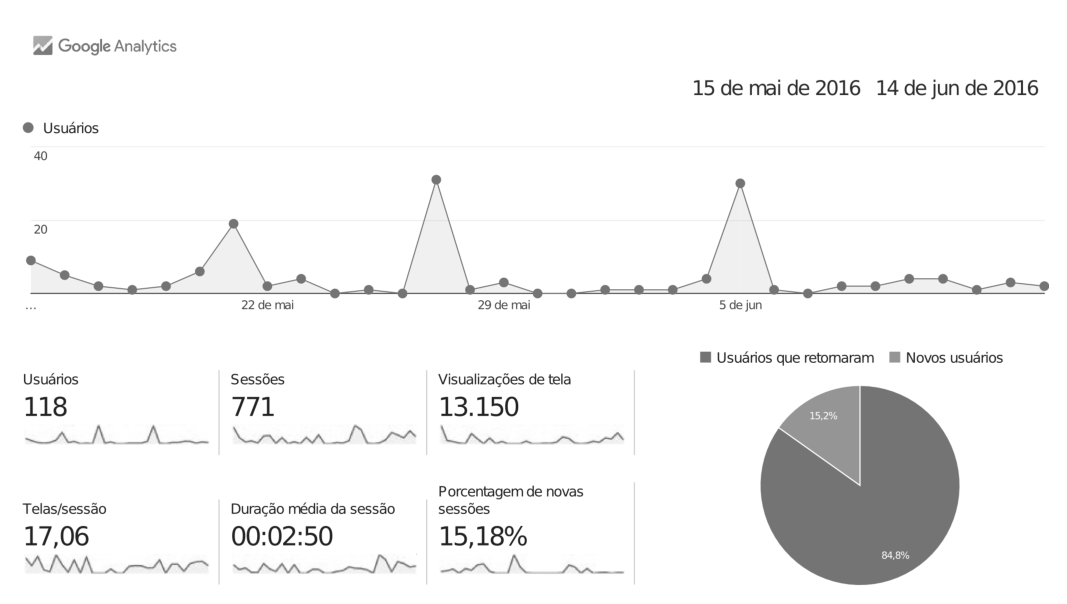
\includegraphics[width=0.8\textwidth]{figuras/analytics_acesso.eps} 
  \caption{Gráficos gerados pelo Google \textit{Analytics}.}
  \label{google_analytics}
\end{figure}

A partir do Google \textit{Analytics} foi possível classificar o principal público do aplicativo através de informações como o sexo, idade e monitoramento do aplicativo como de suas exceções (\textit{crash}) e quais são as telas visualizadas pelos usuários. Como pode ser observado na figura com a utilização do sistema Google \textit{Analytics} foi possível verificar a quantidade usuários do sistema, o tempo de duração média das sessões dos usuários, o percentual de novas sessões dentre outras informações pertinentes sobre a utilização do sistema.

\section*{Considerações finais sobre o capítulo}

\noindent Neste capítulo foi apresentado os resultados obtidos pela implantação do sistema ``\acrshort{uft} Serviços'', sendo apresentado o acordo de nível de serviço (SLA), o \textit{software}, os resultados dos testes realizados e as ferramentas de monitoramento.

Os resultados apresentados neste capítulo foram bastante satisfatórios pois foi possível ter uma visão geral sobre o potencial que aplicação terá a longo prazo. A implantação final do sistema ``\acrshort{uft} Serviços'' em produção irá proporcionar um sistema com desempenho satisfatório, uma boa taxa de aceitação devido ao excelente resultado obtido obtido pela aplicação do SUS e um ambiente de teste e monitoramento para a verificação do comportamento da aplicação durante a utilização dos usuários.


% ----------------------------------------------------------------------------------------------------- %
% Conclusão
% ----------------------------------------------------------------------------------------------------- %

\chapter{Conclusão e Trabalhos Futuros}

\noindent Neste capítulo é apresentado as conclusões obtidas através da execução deste trabalho, sendo apresentado os principais ganhos obtidos com a implantação do sistema, as sugestões para pesquisas futuras e os resultados adicionais obtidos pela implantação do sistema ``\acrshort{uft} Serviços''.

Como pode ser observado no Capítulo Resultados o sistema ``\acrshort{uft} Serviços'' apresenta um bom nível de usabilidade, desempenho e com implementações de medidas de segurança que visam manter a privacidade dos usuários do sistema.

Após a implantação do ``\acrshort{uft} Serviços'', foi constatado que o atendimento dos principais itens do levantamento de requisitos presentes na Especificação de Requisitos de \textit{Software} (IEEE 830 - Apêndice I) foram atendidos de forma satisfatória. Com a ressalva que foram realizadas algumas modificações necessárias, através da adição de novos requisitos e remoção de outros em que não seria possível o seu atendimento em um tempo hábil.

A partir da implantação do sistema, foi possível viabilizar o acesso de um aplicativo móvel pela comunidade acadêmica da \acrshort{uft} do campus de Palmas para a abertura e acompanhamento de chamados de forma acessível. Possibilitando a criação de chamados de forma detalhada, através do fornecimento de informações como a localização, foto e descrições em detalhes do problema. Sendo que o principal objetivo deste trabalho foi alcançado, pois com a implantação do sistema foi possibilitou um canal de comunicação direto com os setores responsáveis pelo atendimento da demanda, proporcionando o acompanhamento do andamento das ordens de serviços por toda a comunidade acadêmica do campus.

A aplicação do \acrshort{itil} v3 como base para o gerenciamento da implantação do sistema foi bastante produtivo, pois foi a partir da aplicação das boas práticas para gerenciamento de serviços de \acrshort{ti} presentes no ciclo de vida de serviços do \acrshort{itil} foi possível obter bons resultados quanto a gestão dos serviços oferecidos pelo \textit{software}.

A partir criação de um ambiente de integração contínua proporcionou uma mecanismo automatizado para a execução de testes, compilação (\textit{build}) e atualização do sistema \textit{deploy}, facilitando uma integração melhor de novas funcionalidades que o sistema pode demandar em uma futura atualização de seus requisitos.

Outro ponto a ressaltar, foi que a aplicação do \acrshort{itil} v3 em conjunto com a metodologia de desenvolvimento ágil \textit{Scrum} foram fundamentais para desenvolvimento e implantação do sistema. Pois através destes método foi possível obter uma melhor organização do processo de criação do \textit{software} e implantação de novos serviços.

\section{Sugestões para Trabalhos Futuros}

\noindent Um possível tema para a realização de uma pesquisa futura deste trabalho seria a partir dos dados gerados pelo sistema, realizar uma análise a partir da aplicação de técnicas de mineração de dados para extração de informações contidas em sua base de dados.

Uma outra sugestão para a realização de uma nova pesquisa seria através da proposta de implementação do cliente móvel para outras plataformas do mercado, como por exemplo para o sistema  \acrshort{ios} e Windows Phone. 

Outra abordagem para a expansão do sistema consistiria no mapeamento do patrimônio da instituição, a partir da utilização de código de barras ou \gls{qrcode}. Tal abordagem em conjunto com o mapeamento da base de dados do patrimônio da instituição possibilitaria o preenchimento automático do formulário de abertura do chamado, bem como a criação de um histórico referente ao número de vezes que um dado patrimônio passou pelo processo de manutenção, podendo agilizar o processo de substituição de um patrimônio.

Uma sugestão de trabalho futuro está na implementação de um sistema de recuperação de informação que consiste em salvar os dados do usuário em uma base de dados local durante momentos de instabilidade de conexão com a internet. Outra sugestão está na realização de mais testes para verificação da qualidade e segurança do \textit{software}, tais como: Teste de Disponibilidade, Teste de Recuperação, Teste de Regressão, Teste Funcional e Teste de Configuração.

% ----------------------------------------------------------------------------------------------------- %
% Apêndice
% ----------------------------------------------------------------------------------------------------- %

\chapter{Apêndice}

\section*{Apêndice I}

\includepdf[pages={1-}]{apendice/srs_ieee830.pdf}

\section*{Apêndice II}

\includepdf[pages={1-}]{apendice/form_sus.pdf}

\section*{Apêndice III}

\includepdf[pages={1-}]{apendice/perfil_sus.pdf}

\section*{Apêndice IV}

\includepdf[pages={1-}]{apendice/sla_uft_servicos.pdf}

% ----------------------------------------------------------------------------------------------------- %
% Anexos
% ----------------------------------------------------------------------------------------------------- %

\chapter{Anexos}

\section*{Anexo I}

\includepdf[pages=-]{anexos/secretaria_acad_alunos.pdf}

\section*{Anexo II}

\includepdf[pages=-]{anexos/perfil_servidores.pdf}

\backmatter 
\singlespacing   % espaçamento simples
% ----------------------------------------------------------------------------------------------------- %
% Bibliografia
% ----------------------------------------------------------------------------------------------------- %
%\bibliographystyle{abntex2-num} 
\bibliography{exemplo}
\end{document}